% Options for packages loaded elsewhere
\PassOptionsToPackage{unicode}{hyperref}
\PassOptionsToPackage{hyphens}{url}
%
\documentclass[
]{book}
\usepackage{lmodern}
\usepackage{amsmath}
\usepackage{ifxetex,ifluatex}
\ifnum 0\ifxetex 1\fi\ifluatex 1\fi=0 % if pdftex
  \usepackage[T1]{fontenc}
  \usepackage[utf8]{inputenc}
  \usepackage{textcomp} % provide euro and other symbols
  \usepackage{amssymb}
\else % if luatex or xetex
  \usepackage{unicode-math}
  \defaultfontfeatures{Scale=MatchLowercase}
  \defaultfontfeatures[\rmfamily]{Ligatures=TeX,Scale=1}
\fi
% Use upquote if available, for straight quotes in verbatim environments
\IfFileExists{upquote.sty}{\usepackage{upquote}}{}
\IfFileExists{microtype.sty}{% use microtype if available
  \usepackage[]{microtype}
  \UseMicrotypeSet[protrusion]{basicmath} % disable protrusion for tt fonts
}{}
\makeatletter
\@ifundefined{KOMAClassName}{% if non-KOMA class
  \IfFileExists{parskip.sty}{%
    \usepackage{parskip}
  }{% else
    \setlength{\parindent}{0pt}
    \setlength{\parskip}{6pt plus 2pt minus 1pt}}
}{% if KOMA class
  \KOMAoptions{parskip=half}}
\makeatother
\usepackage{xcolor}
\IfFileExists{xurl.sty}{\usepackage{xurl}}{} % add URL line breaks if available
\IfFileExists{bookmark.sty}{\usepackage{bookmark}}{\usepackage{hyperref}}
\hypersetup{
  pdftitle={Coding Your Future: A Guidebook for Students},
  pdfauthor={Duncan Hull at the University of Manchester and illustrated by Bryan Mathers at Visual Thinkery},
  hidelinks,
  pdfcreator={LaTeX via pandoc}}
\urlstyle{same} % disable monospaced font for URLs
\usepackage{longtable,booktabs}
\usepackage{calc} % for calculating minipage widths
% Correct order of tables after \paragraph or \subparagraph
\usepackage{etoolbox}
\makeatletter
\patchcmd\longtable{\par}{\if@noskipsec\mbox{}\fi\par}{}{}
\makeatother
% Allow footnotes in longtable head/foot
\IfFileExists{footnotehyper.sty}{\usepackage{footnotehyper}}{\usepackage{footnote}}
\makesavenoteenv{longtable}
\usepackage{graphicx}
\makeatletter
\def\maxwidth{\ifdim\Gin@nat@width>\linewidth\linewidth\else\Gin@nat@width\fi}
\def\maxheight{\ifdim\Gin@nat@height>\textheight\textheight\else\Gin@nat@height\fi}
\makeatother
% Scale images if necessary, so that they will not overflow the page
% margins by default, and it is still possible to overwrite the defaults
% using explicit options in \includegraphics[width, height, ...]{}
\setkeys{Gin}{width=\maxwidth,height=\maxheight,keepaspectratio}
% Set default figure placement to htbp
\makeatletter
\def\fps@figure{htbp}
\makeatother
\usepackage[normalem]{ulem}
% Avoid problems with \sout in headers with hyperref
\pdfstringdefDisableCommands{\renewcommand{\sout}{}}
\setlength{\emergencystretch}{3em} % prevent overfull lines
\providecommand{\tightlist}{%
  \setlength{\itemsep}{0pt}\setlength{\parskip}{0pt}}
\setcounter{secnumdepth}{5}
\ifluatex
  \usepackage{selnolig}  % disable illegal ligatures
\fi
\usepackage[]{natbib}
\bibliographystyle{apalike}

\title{Coding Your Future: A Guidebook for Students}
\author{Duncan Hull at the University of Manchester and illustrated by Bryan Mathers at Visual Thinkery}
\date{}

\begin{document}
\maketitle

{
\setcounter{tocdepth}{1}
\tableofcontents
}
\hypertarget{welcome-to-your-future}{%
\chapter*{Welcome to your future}\label{welcome-to-your-future}}
\addcontentsline{toc}{chapter}{Welcome to your future}

\begin{figure}

{\centering \includegraphics[width=1\linewidth]{images/Coding your future - Title} 

}

\end{figure}

Hello and welcome to \emph{Coding Your Future}, the guidebook that will help you to design, build, test, debug and code your future in computing. This guidebook is aimed at students in higher education, both those studying Computer Science as part of their degree or those from other disciplines with an interest in computing.

This guidebook (also available as \href{https://www.cdyf.me/cdyf.pdf}{cdyf.pdf} and \href{https://www.cdyf.me/cdyf.epub}{cdyf.epub}) supports second year teaching at the University of Manchester, but it DOES NOT MATTER:

\begin{itemize}
\tightlist
\item
  what \emph{stage} of your degree you are at, from first year through to final year
\item
  what \emph{level} you are studying at, foundation, undergraduate or postgraduate
\item
  what \emph{subject} you are studying, provided that you are computationally curious
\item
  what \emph{institution} you are studying at, this book is University and institution agnostic
\item
  \emph{where} in the world you are studying
\end{itemize}

So there is probably something in this guidebook for \emph{any} student of computing. 👨🏿‍💻👨‍💻👩🏽‍💻👩‍💻👨🏿‍💻

\hypertarget{picturethis}{%
\section{Visualising your future}\label{picturethis}}

A lot of self-help literature can be dry, dull, textbooky and boring with few illustrations and conversations.

\begin{figure}

\includegraphics[width=0.32\linewidth]{images/Alicesadventuresinwonderland1898} 
\includegraphics[width=0.32\linewidth]{images/Alicesadventuresinwonderland1898} 
\includegraphics[width=0.32\linewidth]{images/Alicesadventuresinwonderland1898} \caption{The cover of the 1898 edition of the novel \emph{\href{https://en.wikipedia.org/wiki/Alice\%27s_Adventures_in_Wonderland}{Alice's Adventures in Wonderland}}. Public domain image via Wikimedia Commons \href{https://w.wiki/327E}{w.wiki/327E}}\label{fig:aiw-fig}
\end{figure}



In the novel \emph{\href{https://en.wikipedia.org/wiki/Alice\%27s_Adventures_in_Wonderland}{Alice's Adventures in Wonderland}} \citep{wonderland}, the heroine Alice is looking at book her sister is reading:

\begin{quote}
Alice was beginning to get very tired of sitting by her sister on the bank, and of having nothing to do: once or twice she had peeped into the book her sister was reading, but it had no pictures or conversations in it, ``and what is the use of a book,'' thought Alice ``without pictures or conversations?'' -- See \href{https://www.gutenberg.org/files/11/11-h/11-h.htm\#chap01}{gutenberg.org} \citep{wonderland}
\end{quote}

So this book uses pictures and conversations wherever possible to help you understand and visualise your future.

\hypertarget{vaccine}{%
\section{Your future aims}\label{vaccine}}

This guidebook aims to help you develop stronger habits of mind, body and soul using five key ingredients:

\begin{enumerate}
\def\labelenumi{\arabic{enumi}.}
\tightlist
\item
  \textbf{Code:} Instructions contained in this guidebook
\item
  \textbf{Data:} Facts, statistics and images collected together for your analysis
\item
  \textbf{You:} Activities for you to do in addition to reading
\item
  \textbf{Futures:} Possible futures for you to think about. Try not to dwell on the past. Think about the future. \citep{thinkaboutthefuture, wroteforluck} Think about \emph{your} future.
\item
  \textbf{Me:} Hello, my name is Duncan. I'm your tour guide here. If you're feeling a bit lost, follow me.
\end{enumerate}

\begin{figure}

{\centering 
\includegraphics[width=0.69\linewidth]{images/Hello-my-name-is-Duncan} 

}

\caption{Hello my name is Duncan. If you're feeling a bit lost, follow me. Image adapted from ``Hello my name is sticker'' by Eviatar Bach, public domain \href{https://w.wiki/32RV}{w.wiki/32RV}}\label{fig:hello-my-name-fig}
\end{figure}



Coding your future explores techniques for making career decisions, job searching, submitting applications and competing successfully in interviews and the workplace.

Alongside these practical engineering issues, this guidebook also encourages you to \emph{design your future} by taking a step back and reflecting on the bigger picture. You will apply \href{https://en.wikipedia.org/wiki/Computational_thinking}{computational thinking} techniques, to reflect on who you are, what your story is, how you communicate with other people and what your experience is. As there is a computational theme, you will also need to reflect on what your inputs and outputs (\href{https://en.wikipedia.org/wiki/Input/output}{I/O}) are, both now and in the future. You'll also need to think about what recipes (or algorithms) you might start experimenting with

This guidebook tackles professional issues in computing, for those with and without Computer Science degrees in the early stage of their careers.

\hypertarget{nilo}{%
\section{What you won't learn}\label{nilo}}

What you won't learn This guidebook will NOT teach you how to write code, there's already lots of fantastic resources to help you do that. We discuss some of them in chapter on \protect\hyperlink{computing}{computing your future}.

\hypertarget{bilo}{%
\section{Learning your future}\label{bilo}}

So what \emph{will} you learn from this guidebook? After reading this guidebook, watching the videos and doing the exercises you will be able to:

\begin{enumerate}
\def\labelenumi{\arabic{enumi}.}
\tightlist
\item
  Improve your self-awareness by describing who you are, what motivates you and your strengths and weaknesses
\item
  Decide on a job search strategy and identify employers, sectors and roles that are of interest to you\\
\item
  Improve your written communication skills both for job applications and communicating with other people
\item
  Plan and prepare competitive written applications using standard techniques including CVs, covering letters, application forms and digital profiles
\item
  Compete successfully in interviews and assessment centres by preparing for technical and non-technical questions
\item
  Plan further steps in your career such as promotion, postgraduate study \& research, alternative employment and longer term goals
\item
  Search and navigate a large ``wordbase'' (this guidebook and the work it cites). A wordbase is like a \href{https://en.wikipedia.org/wiki/Codebase}{codebase}, only written predominantly in natural language.
\end{enumerate}

\hypertarget{prereq}{%
\subsection{Your future prerequisites}\label{prereq}}

As the title of this guidebook implies, there is a computational flavour here, but you do not have to be studying Computer Science to benefit. There are two main target audiences for this guidebook:

\begin{enumerate}
\def\labelenumi{\arabic{enumi}.}
\tightlist
\item
  Undergraduate and postgraduate students studying Computer Science as a major or minor part of their degree. This includes software engineering, artificial intelligence, human-computer interaction (HCI), information systems, health informatics, data science, gaming, cybersecurity and all the other myriad flavours of Computer Science
\item
  Undergraduate and postgraduate students studying \emph{any} subject, with little or no Computer Science at all. You are curious to know about what role computing could play in your future career because computing is too important to be left to Computer Scientists.
\end{enumerate}

So the prerequisites for this book are that you are studying (or have studied) at University where English is one of the main spoken languages. You \emph{may} have some experience already, either casual, voluntary or otherwise, but this book does \textbf{not} assume that you have already been employed in some capacity.

\hypertarget{gut}{%
\subsection{Gutting your future}\label{gut}}

Don't read this book, gut it! Reading this book from cover to cover like a novel is not recommended. That would be foolish.

\begin{figure}

{\centering 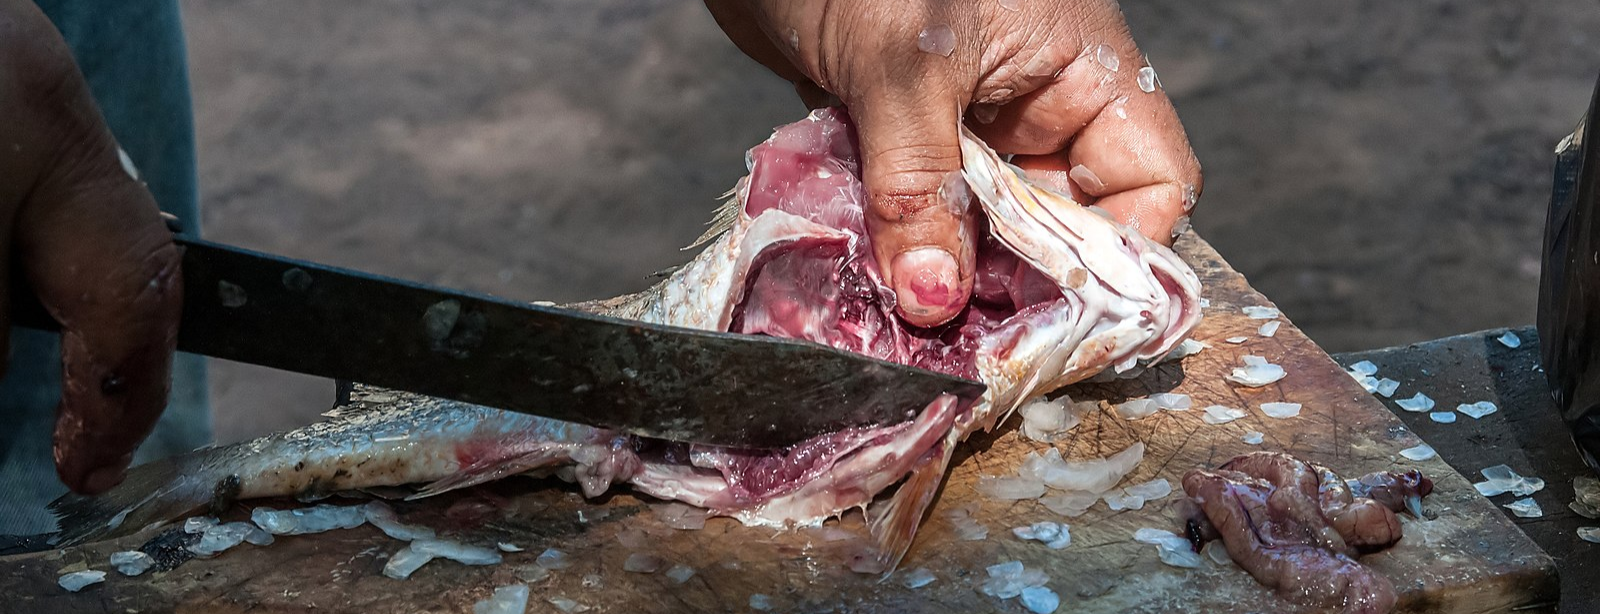
\includegraphics[width=1\linewidth]{images/fish-gutting} 

}

\caption{Don't read this book, gut it like a fish. Gutting fish in Isla Margarita image by Wilfredor via Wikimedia commons \href{https://w.wiki/_23m}{w.wiki/\_23m}}\label{fig:gut-fig}
\end{figure}



Instead of reading this book, I suggest you follow the advice given to historian \href{https://en.wikipedia.org/wiki/William_Woodruff}{William Woodruff} about reading books when he was at University:

\begin{quote}
``You don't READ books, you GUT them!'' \citep{nabend} 🐟
\end{quote}

So, gut this book like a fish. Identify the chapters that are most useful to you (the flesh), and skip the rest (the guts). Which chapters are flesh and which are guts will depend on what stage of the journey you are at. This guidebook is designed to be as ``guttable'' as possible.
To aid gutting, the version published at \href{https://www.cdyf.me/}{cdyf.me} has a built in search and tables of contents. Before you can gut the fish, you'll need an anatomical map shown in figure \ref{fig:map-fig}.

\hypertarget{mapping}{%
\section{Mapping your future}\label{mapping}}

This guidebook is split into three parts. The first part is on \href{bothering.html}{designing your future} while the second is on \href{debugging.html}{building and testing your future} shown in the map in figure \ref{fig:map-fig}. The final part is a \href{ruling.html}{help} section, for rebooting your future. Let's look in a bit more detail at the content of each of the three parts of this guidebook:

\begin{figure}

{\centering \includegraphics[width=1\linewidth]{images/Course Map} 

}

\caption{Mapping your future: Each yellow dot on this diagram is a chapter in \emph{Coding Your Future}. The chapters on the left tackle design issues like \emph{who are you}? Chapters on the right tackle the practicalities of executing and testing your career choices, such as \emph{debugging your CV}. Mapping your Future artwork by \href{https://visualthinkery.com/}{Visual Thinkery} is licenced under \href{https://creativecommons.org/licenses/by-nd/4.0/}{CC-BY-ND}}\label{fig:map-fig}
\end{figure}



\hypertarget{parti}{%
\subsection{Designing your future}\label{parti}}

The first six chapters of this guidebook look at what engineers call \emph{design}. When you build anything, a bridge, a piece of software, a car or a plane you'll need to do some design like the blueprint in figure \ref{fig:brooklyn-fig}

\begin{figure}

{\centering 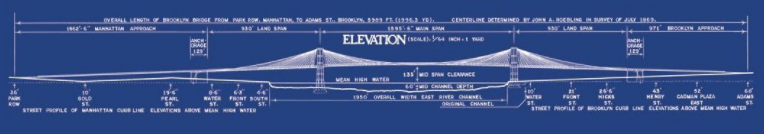
\includegraphics[width=1\linewidth]{images/brooklyn-bridge-blueprint} 

}

\caption{Designing your future is about drawing up a \href{https://en.wikipedia.org/wiki/Blueprint}{blueprint}, like this one for the elevation of the \href{https://en.wikipedia.org/wiki/Brooklyn_Bridge}{Brooklyn Bridge} in New York. What does your blueprint look like? The chapters on \href{bothering.html}{designing your future} will help you fill in the details.}\label{fig:brooklyn-fig}
\end{figure}



Building a career isn't that different to building anything else, you'll need to do some design work and it will probably be iterative. Designing things often involves asking tricky questions. So when you're designing your future you'll need to cover the following:

\begin{enumerate}
\def\labelenumi{\arabic{enumi}.}
\tightlist
\item
  \href{bothering.html}{Investigating your future} looks at why you should bother reading any of this guidebook
\item
  \href{knowing.html}{Knowing your future} challenges you to reflect on who you are, what makes you unique and why you are here
\item
  \href{wellbeing.html}{Nurturing your future} encourages you to take care of your mental and physical health
\item
  \href{communicating.html}{Writing your future} explores your soft skills, and how they complement your hard skills and why employers value them so much
\item
  \href{experiencing.html}{Experiencing your future} asks you to reflect on your work experience and help identify where you can improve it
\item
  \href{computing.html}{Computing your future} looks at the role computing can play in your career, with or without a Computer Science degree
\end{enumerate}

\hypertarget{partii}{%
\subsection{Building and testing your future}\label{partii}}

The next six chapters look at building and testing your future, what engineers like to call \emph{implementation}, \emph{execution} or \emph{construction} shown in figure \ref{fig:manhattan-fig}

\begin{figure}

{\centering 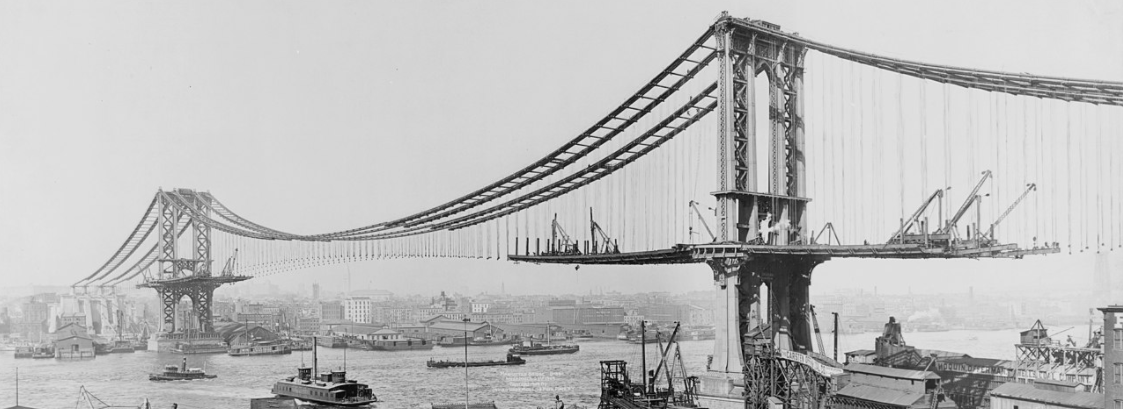
\includegraphics[width=1\linewidth]{images/manhattan_bridge} 

}

\caption{Just like the \href{https://en.wikipedia.org/wiki/Manhattan_Bridge}{Manhattan Bridge}, your future will be easier to build once you've done some design. Even a sketch will do. Design questions are covered in the first part of this guidebook: \href{bothering.html}{designing your future}. Picture of the Manhattan bridge under construction in 1909 adapted from a public domain image via Wikimedia commons \href{https://w.wiki/32Rg}{w.wiki/32Rg}}\label{fig:manhattan-fig}
\end{figure}



Once you've started to answer the design questions in the first part, you can start to implement (or build) your career and think about what the next steps will be.

\begin{enumerate}
\def\labelenumi{\arabic{enumi}.}
\tightlist
\item
  \href{debugging.html}{Debugging your future} looks at debugging your written communication such as covering letters, application forms and digital portfolios.
\item
  \href{finding.html}{Finding your future}, looks at where and how can you look for interesting opportunities
\item
  \href{interviewing.html}{Speaking your future}, looks how can you turn interviews to your advantage and negotiate any offers you receive
\item
  \href{surviving.html}{Surviving your future} looks at the next steps. Once you've landed a job, how will you survive and thrive outside (and after) University
\item
  \href{studying.html}{Researching your future} discusses if a Masters degree or a PhD right for you?
\item
  \href{broadening.html}{Broadening your future} encourages you to broaden your horizons. Maybe you want to start your own business and employ others or you'd like to work in the non-profit or public sector? Perhaps you could be a freelancer or contractor? The possibilities are endless.
\end{enumerate}

\hypertarget{partiii}{%
\subsection{Supporting your future}\label{partiii}}

The third part of this book, contains supporting material that will help the design, build and test phases described above. You'll need good support to help with the stresses and strains of building your future shown in \ref{fig:clifton-fig}

\begin{figure}

{\centering 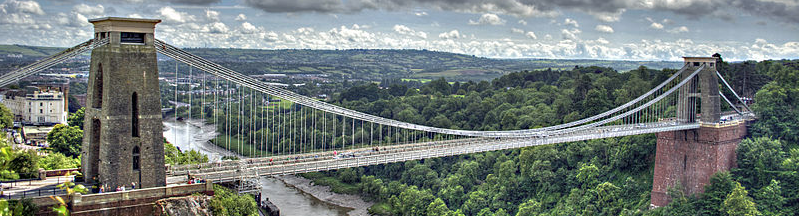
\includegraphics[width=1\linewidth]{images/clifton} 

}

\caption{The \href{https://en.wikipedia.org/wiki/Clifton_Suspension_Bridge}{Clifton Suspension Bridge} in Bristol has supporting chains which can move when heavy loads pass over the Avon valley bridge. You'll need good support to cope with the stresses and strains of building your future. Clifton suspension bridge picture adapted from original by Nic Trott via Wikimedia commons \href{https://w.wiki/32tu}{w.wiki/32tu}}\label{fig:clifton-fig}
\end{figure}



\begin{enumerate}
\def\labelenumi{\arabic{enumi}.}
\tightlist
\item
  \href{ruling.html}{Ruling your future} provides \emph{Ten Simple Rules for Coding your Future}, this book in a nutshell
\item
  \href{sampling.html}{Reading their future} invites you to put yourself in the employers shoes by reading some CVs
\item
  \href{notjustlondon.html}{Moving your future} looks at opportunities outside of capital cities like London
\item
  \href{listening.html}{Listening to your future} invites you to hear students stories of their transition from education to employment
\item
  \href{verbsfirst.html}{Actioning your future} gets you to think about your actions by emphasising verbs on your job applications
\item
  \href{scheduling.html}{Scheduling your future} invites you to set aside an hour each week for tackling the issues described in this book
\item
  \href{reading.html}{Reading your future} everything we've cited in this guidebook, because books are good for your soul
\end{enumerate}

\hypertarget{themes}{%
\section{Your future themes}\label{themes}}

This guidebook aims to help you build a bridge from where you are now to where you'd like to be in the future. Each chapter of the book contains the following recurring themes:

\begin{figure}

{\centering 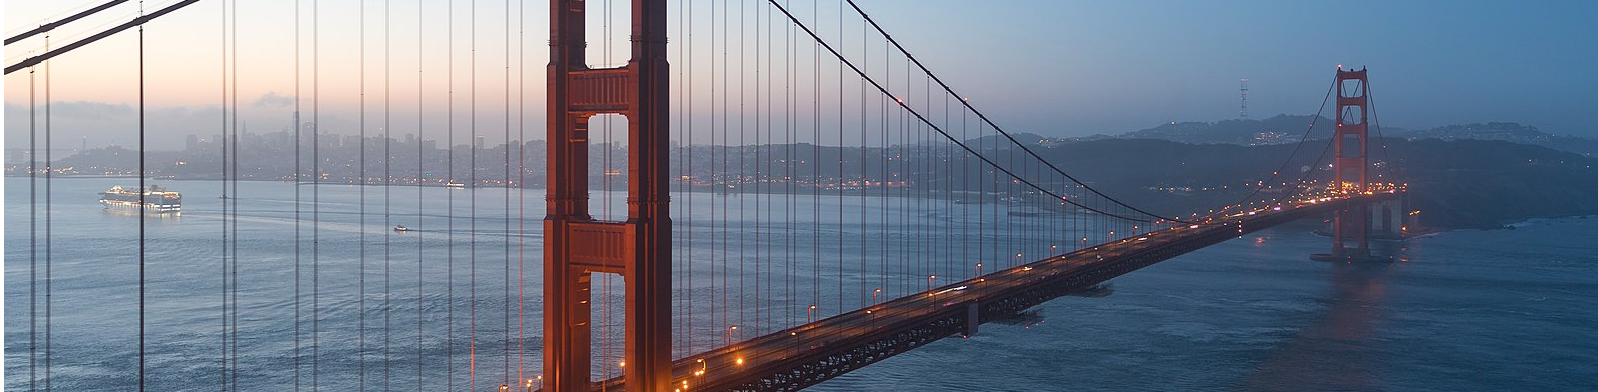
\includegraphics[width=1\linewidth]{images/goldengate} 

}

\caption{The iconic \href{https://en.wikipedia.org/wiki/Golden_Gate_Bridge}{Golden Gate Bridge} in California, adapted from an original picture by Frank Schulenburg (CC BY-SA) on Wikimedia Commons \href{https://w.wiki/37kY}{w.wiki/37kY}}\label{fig:goldengate-fig}
\end{figure}



\begin{enumerate}
\def\labelenumi{\arabic{enumi}.}
\tightlist
\item
  \textbf{Learning} your future: What you will learn from any given chapter
\item
  \textbf{Watching} your future: videos and animations for you to watch
\item
  \textbf{Listening} to your future: audio and podcasts for you to listen to
\item
  \textbf{Speaking} your future: articulating from a script or by improvisation
\item
  \textbf{Discussing} your future: \href{https://en.wikipedia.org/wiki/Breakpoint}{breakpoints} invite you to stop your code from executing and think about the variables and parameters you are using. Can they be improved? Reflect and discuss.
\item
  \textbf{Reading} your future: reading stuff because its good for your mind, body and soul. Read The Friendly Manual. \href{https://en.wikipedia.org/wiki/RTFM}{RTFM}. Read THIS Friendly Manual.
\item
  \textbf{Writing} your future: written exercises using natural language
\item
  \textbf{Quizzing} your future: quick quizzes to be done in \href{scheduling.html}{real-time live scheduled sessions} (synchronously) and in your own time (asynchronously)
\item
  \textbf{Assessing} your future: activities to be assessed by yourself, your peers, an employer or an academic (depending on who and where you are)
\item
  \textbf{Challenging} your future: coding challenges are designed to take you out of your comfort zone by encouraging you to experiment with your thoughts, discussions and actions
\item
  \textbf{Signposting} your future: the most useful resources that I recommend you read, listen to or watch
\end{enumerate}

\hypertarget{thanks}{%
\section{Acknowledgements}\label{thanks}}

The content of this book is based on hundreds of conversations I have had with students of (mainly) Computer Science and Maths with some Physics and Engineering, since 2012. I've also spoken to many of their employers too.

\hypertarget{students}{%
\subsection{Standing on the shoulders of students}\label{students}}

First and foremost, I'd like to thank all the students who have helped with this book, both directly and indirectly.

\begin{quote}
``If I have seen further it is by \href{https://en.wikipedia.org/wiki/Standing_on_the_shoulders_of_giants}{standing on the shoulders of students}.'' \citep{newton}
\end{quote}

So, if you have studied some flavour of Computer Science at the University of Manchester since 2012, there's a high probability you have contributed to this book. Thank you for having the courage to tell me your stories. Thank you for being ambitious, hard working, talented, fearless, creative, inspirational and listening to me. It has been my pleasure and privilege to work with you all.

\begin{figure}

{\centering \includegraphics[width=1\linewidth]{images/bbcbreakfastsofa} 

}

\caption{Posing on the \href{https://en.wikipedia.org/wiki/BBC_Breakfast}{BBC Breakfast} red sofa with the winning student team at the BBC / Barclays University Technology Challenge (UTC) in \href{https://en.wikipedia.org/wiki/MediaCityUK}{MediaCityUK}, Salford, Greater Manchester}\label{fig:unnamed-chunk-2}
\end{figure}



I'd especially like to thank industrial experience (IE) students who have completed a year in industry as part of their degree as well as those who have done summer internships, either as part of the Master of Engineering (MEng) program or otherwise, particularly Luke Beamish and Petia Davidova. In addition, the \href{http://www.pass.manchester.ac.uk}{PASS leaders} and facilitators, \href{https://unicsmcr.com/}{UniCSmcr.com}, \href{https://github.com/unicsmcr/hacksoc.com}{HackSoc}, \href{https://github.com/cssoc}{CSSoc} and \href{https://github.com/Man-UP}{Manchester Ultimate Programming} members have all been influential on the content of this book. I've learned heaps by manually trawling through thousands of your CVs too, so if you've shown me a copy of your CV, thanks! If you sent me a CV and I didn't reply, I apologise. There are limits to what is humanly possible. The chapters on \href{debugging.html}{debugging your future} (self assessment) and \href{sampling.html}{reading their future} (peer assessment) are based on the most common bugs (or are they features?) I've seen in CVs.

So, thank you students for being studious. 🙏

\hypertarget{employers}{%
\subsection{Thank you employers}\label{employers}}

Thanks to all the organisations who have employed students from the Department of Computer Science as either summer interns, year long placements or graduates. A big chunk of this guidebook documents their experience of employers and their graduate recruitment programs.

Thanks to Niall Beard and \href{https://github.com/sharifsalah}{Sharif Salah} at Google for introducing me to Google's Technical Writing course. \citep{googling}

So, thanks employers for employing our students. 🙏

\hypertarget{colleagues}{%
\subsection{Thank you colleagues}\label{colleagues}}

I've also had significant support from colleagues in the Department of Computer Science (\href{https://twitter.com/csmcr}{@csmcr}) and support staff at the University of Manchester. (\href{https://twitter.com/ManUniCareers}{@ManUniCareers}, \href{https://twitter.com/alumniUoM}{@alumniUoM}, \href{https://twitter.com/OfficialUoM}{@OfficialUoM})

I would especially like to thank \href{https://en.wikipedia.org/wiki/James_John_Miles}{Jim Miles} for encouraging me to write a book shortly after he offered me a job. I thought he was joking (about the book) but it actually turned out to be another one of Jim's great ideas. Thanks Jim. 🙏

I'd also like to thank the only three people in the whole world who've had the misfortune of reading all of my PhD thesis; \href{https://en.wikipedia.org/wiki/Robert_David_Stevens}{Robert Stevens}, \href{https://www.ncl.ac.uk/computing/staff/profile/anilwipat.html}{Anil Wipat} and \href{https://en.wikipedia.org/wiki/Steve_Pettifer}{Steve Pettifer}. I suspect it was as painful for you to read as it was for me to write it. Thanks Robert for your relentless patience and giving me a well timed, well aimed kick up the arse (to write this book) in the \href{https://en.wikipedia.org/wiki/Midland_Hotel,_Manchester}{Midland Hotel, Manchester} at the May ball. ⚽️

Thanks to \href{https://en.wikipedia.org/wiki/Carole_Goble}{Carole Goble} for re-teaching me how to write by covering drafts of my MSc thesis in red ink (and swear words 🤬\footnote{the swear words didn't appear until the sixth of seventh draft}) and \href{https://en.wikipedia.org/wiki/Steve_Furber}{Steve Furber} for playing bass in our ``boy band'' \href{http://www.cs.man.ac.uk/~hulld/research.html\#tuningcomplete}{Tuning Complete}.

\hypertarget{academia}{%
\subsubsection{Thanks to academic staff}\label{academia}}

Thanks to past and present academic colleagues, PhD students and teachers at the University of Manchester who have contributed to this guidebook and the environment it was written in. We are bound together by the \protect\hyperlink{weakties}{power of weak ties} alongside stronger forces and friendships. They include (in alphabetical order):

Pinar Alper, Sophia Ananiadou, Mikel Egaña Aranguren, Constantinos Astreos, Terri Attwood, Sam Bail, \href{https://en.wikipedia.org/wiki/Robin_Baker_(biologist)}{Robin Baker}, Richard Banach, Riza Batista-Navarro, Michael Bada, Niall Beard, Sean Bechhofer, Lynne Bianchi, Helena Björn van Praagh, Stewart Blakeway, Petrut Bogdan, Caroline Bowsher, Linda Brackenbury, Judy Brewer, Nick Brown, Mihai Bujanca, Oscar Corcho, Christian Brenninkmeijer, Andy Bridge, Andy Brass, Andy Brown, Gavin Brown, Terry V. Callaghan, Grant Campbell, Angelo Cangelosi, Peter Capon, Andy Carpenter, Nicola Carrier, Barry Cheetham, Ke Chen, Sarah Clinch, Ian Cottam, Brian Cox, Simone Di Cola, Paul Dobson, Clare Dixon, Danny Dresner, Nick Drummond, Warwick Dunn, Doug Edwards, Iliada Eleftheriou, Anas Elhaig, Suzanne Embury, \href{https://www.uoguelph.ca/mcb/people/dr-michael-j-emes}{Michael Emes}, Alvaro Fernandes, Jonathan Ferns, Michele Filannino, Nick Filer, Paul Fisher, Steve Furber, Andre Freitas, Aphrodite Galata, Matthew Gamble, Jim Garside, Kristian Garza, Chris Gilbert, Danielle George, Richard Giordano, Birte Glimm, Carole Goble, Rafael Gonçalves, Antoon Goderis, Roy Goodacre, Bernardo Cuenca Grau, Peter R. Green, \href{https://en.wikipedia.org/wiki/Keith_Gull}{Keith Gull}, John Gurd, Luke Hakes, Robert Haines, Guy Hanke, Simon Harper, \href{https://www.coventry.ac.uk/research/research-people/professor-phil-harris/}{Phil Harris}, Jonathan Heathcote, \href{https://github.com/eldog}{Lloyd Henning}, Gareth Henshall, Andrew Horn, Farid Kahn, Matthew Horridge, Ian Horrocks, Toby Howard, Roger Hubbold, Luigi Iannone, Jane Ilsley, Jules Irenge, Daniel Jameson, Caroline Jay, Mirantha Jayathilaka, Huw Jones, Simon Jupp, Yevgeny Kazakov, John Keane, Douglas Kell, Catriona Kennedy, Rachel Kenyon, Chris Knight, Joshua Knowles, Dirk Koch, Nikolaos Konstantinou, Christos Kotselidis, Ioannis Kotsiopoulos, Oliver Kutz, Alice Larkin, Peter Lammich, John Latham, Kung-Kiu Lau, \href{https://pureportal.coventry.ac.uk/en/persons/margi-lennartsson-turner}{Margi Lennartsson Turner}, Dave Lester, Peter Li, Zewen Liu, Phil Lord, Mikel Luján, Darren Lunn, Matthew Makin, Nicolas Matentzoglu, Paul Mativenga, Erica McAlister, April McMahon, Merc and members of the \href{https://www.mumc.me.uk/wordpress}{Manchester University Mountaineering Club} (MUMC), Simon Merrywest, Eleni Mikroyannidi, Colin Morris, Norman Morrison, Georgina Moulton, Boris Motik, Christoforos Moutafis, Tingting Mu, Ettore Murabito, Mustafa Mustafa, Javier Navaridas, Kostas Nikolou, Aleksandra Nenadic, Goran Nenadic, Steve McDermott, Jock McNaught, Mary McGee-Wood, Pedro Mendes, Sarah Mohammad-Qureshi, Tim Morris, Jennifer O'Brien, Tim O'Brien, Steve Oliver, Pierre Olivier, Mario Ramirez Orihuela, Stuart Owen, Ali Owrak, Pavlos Petoumenos, Luis Plana, \href{https://www.brookes.ac.uk/ocsld/about-ocsld/staff-profiles/jackie-potter/}{Jackie Potter}, \href{https://en.wikipedia.org/wiki/Malcolm_Press}{Malcolm Press}, Colin Puleston, Paul Nutter, Ignazio Palmisano, Dario Panada, Michael Parkin, Bijan Parsia, Jon Parkinson, Norman Paton, Jeff Pepper, Steve Pettifer, Rishi Ramgolam, Allan Ramsay, Alasdair Rawsthorne, Farshid Rayhan, Alan Rector, Giles Reger, Graham Riley, David Robertson, Jeremy Rodgers, Clare Roebuck, Jeremy Rodgers, Mauricio Jacobo Romero, Nancy Rothwell, William Rowe, Oliver Rhodes, David Rydeheard, Graham Riley, Daniella Ryding, Ulrike Sattler, Ahmed Saeed, Pejman Saeghe, Rizos Sakellariou, Pedro Sampaio, Sandra Sampaio, John Sargeant, Andrea Schalk, Viktor Schlegel, Renate Schmidt, Jonathan Shapiro, Vangelis Simeonidis, \href{https://www.manchester.ac.uk/discover/governance/structure/board-governors/members/liz-sheffield/}{Liz Sheffield}, Bushra Sikander, Kieran Smallbone, Alastair Smith, Stian Soiland-Reyes, Irena Spasic, David Spendlove, Robert Stevens, Alan Stokes, Shoaib Sufi, James Sumner, \href{https://github.com/dj-foxxy}{Peter Sutton}, Neil Swainston, \href{https://www.springer.com/gp/book/9780412303203}{John H. Tallis}, Paul Taplin, Federico Tavella, Chris Taylor, Tom Thomson, Dave Thorne, David Toluhi, \href{https://www.theguardian.com/science/2020/nov/10/tony-trinci-obituary}{Tony Trinci}, Dimitri Tsarkov, Daniele Turi, Jake Vasilakes, Laura Vasques, Delia Vazquez, Giles Velarde, Chiara Del Vescovo, Markel Vigo, Andrei Voronkov, Niels Walet, Alex Walker, Louise Walker, Dieter Wiechart, Igor Wodiany, Katy Wolstencroft, Natalie Wood, Chris Wroe, Crystal Wu, Lisheng Wu, Yifan Xu, Viktor Yarmolenko, Yeliz Yesilada, Serafeim Zanikolas, Xiao-Jun Zeng, Jun Zhao, Liping Zhao, Ning Zhang and Evgeny Zolin.

Optimists will tell you that ``everyone has a book in them\ldots{}'', but pessimists like \href{https://en.wikipedia.org/wiki/Christopher_Hitchens}{Christopher Hitchens} will add that ``\ldots in most cases that's exactly where it should remain''. \citep{everyone}

Despite Hitchens amusing trademark cynicism shown in figure \ref{fig:hitchens-fig}, I am an optimist when it comes to the power of natural languages.

\begin{figure}

{\centering 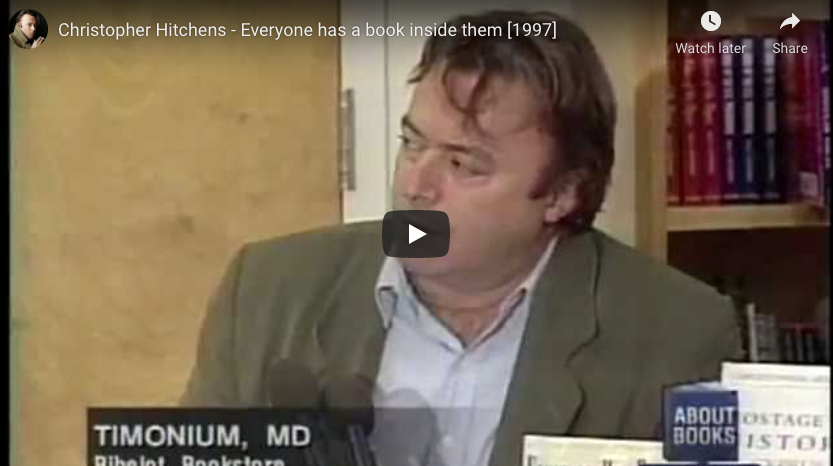
\includegraphics[width=0.99\linewidth]{images/youtube-hitch} 

}

\caption{Christopher Hitchens explains the difference between autobiography and memoir \citep{everyone}}\label{fig:hitchens-fig}
\end{figure}



\hypertarget{psstaff}{%
\subsubsection{Thank you professional services staff}\label{psstaff}}

Thanks also to the superb support staff (past and present) from professional services, especially the Academic Support Office (ACSO), Student Support Office (SSO) and external affairs office in the Kilburn building. Professional services staff continue to make all the magic of teaching and learning possible: Alyx Adams, Cassie Barlow, Jennie Ball-Foster, Emma Bentley, Christine Bowers, Karen Butterworth, Chris Connolly, Ellie Crompton, Jean Davison, Gavin Donald, Miriam Cadney, Chris Calland, Ben Carter, Hannah Cousins, Holly Dewsnip, Tammy Goldfeld, Penney Gordon-Lanes, Amelia Graham, Iain Hart, Kath Hopkins, Lynn Howarth, Yvonne Hung, Susie Hymas, Radina Ivanova, Alex Jones, Jessicca Kateryniuk-Smith, Mike Keeley, Stephanie Lee, Dominic Laing, Gill Lester, Jez Lloyd, Ruth Maddocks, Cameron Macdonald, Tony McDonald, Karon Mee, Anne Milligan, Rachel Mutters, Matthew Oakley, Alyson Owens, Chris Page, Melanie Price, Chris Rhodes, Graham Richardson, Martin Ross, Julian Skyrme, Elaine Sheehan, Angela Standish, Martine Storey, Bernard Strutt, Jannine Thomas, Joseph Tirone, Daisy Towers, Anna Warburton-Ball, Richard Ward, Sarah White, Elizabeth Wilkinson, Andrew Whitmore, Lisa Wright and Mabel Yau.

And Wendy. We all miss you and love you Wendy. \href{https://www.justgiving.com/crowdfunding/byte-cafe}{\#JusticeForWendy} ✊🏽 \href{https://en.wikipedia.org/wiki/Fight_the_Power_(Public_Enemy_song)}{Fight the Power}! ✊🏽 \citep{fightthepower}

So, thank you colleagues for being collegiate. You all make the University of Manchester a \emph{fantastic} place to work, even during a global pandemic. 🙏

\hypertarget{universities}{%
\subsection{Thank you scholars}\label{universities}}

Beyond Manchester there is a wider academic community of scholars that have influenced this guidebook:

\begin{itemize}
\tightlist
\item
  Thanks to \href{https://scholar.google.com/citations?user=CwnKRzMAAAAJ}{Sally Fincher} and Janet Finlay whose report \href{https://kar.kent.ac.uk/53848}{Computing Graduate Employability: Sharing Practice} \citep{fincherreview} has had a big influence on this guidebook.
\item
  Thanks to \href{https://www.gla.ac.uk/schools/computing/staff/quintincutts/}{Quintin Cutts}, \href{https://www.dur.ac.uk/research/directory/staff/?mode=staff\&id=106}{Steven Bradley} and \href{http://eecs.qmul.ac.uk/profiles/waitejanelisa.html}{Jane Waite} for helping me setup and run \href{https://sigcse.cs.manchester.ac.uk/}{SIGCSE journal club}. Thanks to all the \href{https://sigcse.cs.manchester.ac.uk/who/}{journal clubbers} too, many of our journal club conversations have fed directly into the content of this guidebook
\item
  Thanks to \href{https://en.wikipedia.org/wiki/David_J._Malan}{David Malan} (\href{https://cs.harvard.edu/malan/}{@malan}) for \href{https://en.wikipedia.org/wiki/CS50}{CS50} which continues to be an inspiration to me and many others. \citep{cs50, cs50zoom, CS502021} Thanks to \href{https://crisbodnar.github.io/}{Cristian Bodnar} for inviting David to run \href{http://cs50.hacksoc.com}{CS50 in Manchester} in 2017 which was a great introduction to David's work \citep{cs50mcr}
\item
  Thanks to \href{https://en.wikipedia.org/wiki/Laurie_R._Santos}{Laurie Santos} (\href{https://twitter.com/lauriesantos}{@lauriesantos}), for \emph{The Science of Well-being} (TSOWB) \citep{lauriesantos} which was been a significant influence on this book had a gradual but dramatic effect on my personal and professional life
\item
  Thanks to \href{https://en.wikipedia.org/wiki/Hadley_Wickham}{Hadley Wickham} (\href{https://github.com/hadley}{@hadley}) and Garrett Grolemund (\href{https://github.com/garrettgman}{@garrettgman}) for \emph{R for Data Science} \citep{r4ds} which helped me get started with R and bookdown. If you're reading this page in some kind of web browser, the stylesheet used here is re-used from \href{https://r4ds.had.co.nz/}{r4ds.had.co.nz}
\item
  Thanks to Athene Donald at \href{http://occamstypewriter.org/athenedonald/}{Occams Typewriter} and Stephen Curry at \href{https://occamstypewriter.org/scurry/}{Reciprocal Space} for writing entertaining and inspiring blogs
\item
  Thanks to \href{https://en.wikipedia.org/wiki/Jess_Wade}{Jessica Wade} for inspiration, \href{https://wiki-loves-scientists.org.uk/2020/05/21/wiki1000/}{support} and educating me on some of the issues of equality, diversity and inclusion, especially gender and race.
\item
  Thanks to \href{https://www.new.ox.ac.uk/node/1003}{Jonathan Black} (\href{https://twitter.com/JonathanPBlack}{@JonathanPBlack}) for his book \emph{Where am I Going, Can I Have a Map?}, \citep{jonathanblack} his \emph{Financial Times} columns \citep{ft} and videos.
\item
  Thanks to \href{https://en.wikipedia.org/wiki/David_Alan_Walker}{David Alan Walker} for his book \emph{Energy, Plants \& Man} which inspired the conversations and pictures idea behind this book.
\end{itemize}

So thanks scholars for being scholarly. 🎓

\hypertarget{bath}{%
\subsection{Thank you Bath}\label{bath}}

As a graduate of the \href{https://en.wikipedia.org/wiki/Postgraduate_Certificate_in_Education}{Postgraduate Certificate in Education} (PGCE) in Science at the \href{https://en.wikipedia.org/wiki/University_of_Bath}{University of Bath} (graduated 2011), I have been heavily influenced by the fantastic work of PGCE science course leaders Caroline Padley (Physics), Steve Cooper (Chemistry), Malcolm Ingram (Biology) and fellow students on the course.

\begin{figure}

{\centering 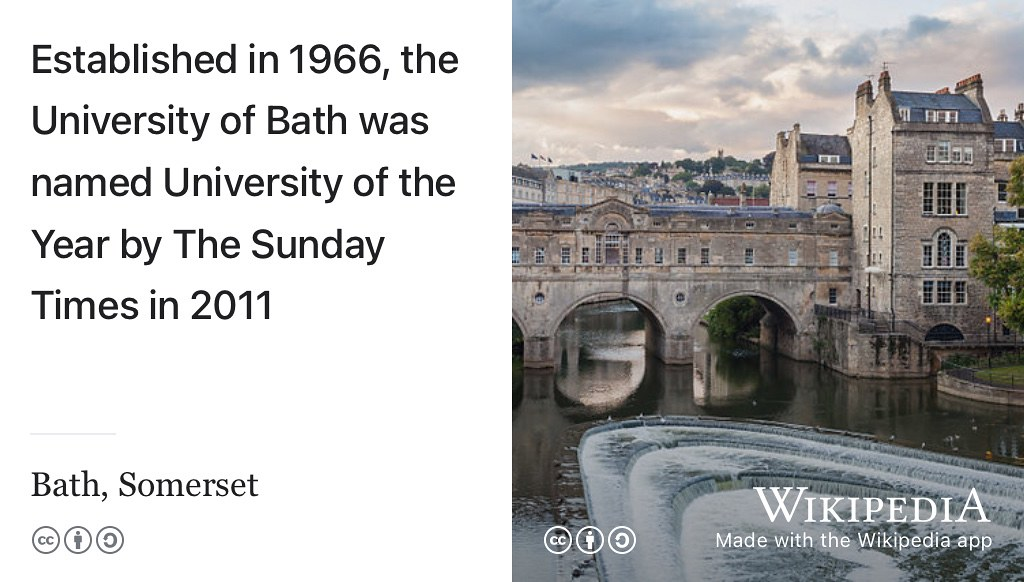
\includegraphics[width=1\linewidth]{images/bath-panorama} 

}

\caption{Panorama of the world heritage site and Georgian City of \href{https://en.wikipedia.org/wiki/Bath,_Somerset}{Bath, Somerset}. Image cropped from an original by David Iliff available under CC BY-SA 3.0 license via Wikimedia Commons at \href{https://w.wiki/32BS}{w.wiki/32BS}}\label{fig:bath-fig}
\end{figure}



Thanks Bath for the initial teacher training (ITT), the medicinal \href{https://en.wikipedia.org/wiki/Aquae_Sulis}{Aquae Sulis} and the beautiful \href{https://en.wikipedia.org/wiki/Cotswolds}{Cotwolds} Area of Outstanding Natural Beauty (\href{https://en.wikipedia.org/wiki/Area_of_Outstanding_Natural_Beauty}{AONB}). 🙏

\hypertarget{shaftesbury}{%
\subsection{Thank you Shaftesbury}\label{shaftesbury}}

Thanks to Stuart Ferguson, David Booth, Chris Almond, David Ball, Caroline Dallimore, Mr Travers, Caroline Moss and all the other staff and students at \href{https://en.wikipedia.org/wiki/Shaftesbury_School}{Shaftesbury School} who hosted my first PGCE teaching placement. Thanks also to my fellow Shaftesbury/Bath trainees Katharine Platt, Harriet Edwards, Vicky Dury and Joan Shaw for sharing their hard won knowledge through \href{https://en.wikipedia.org/wiki/Peer_learning}{peer learning}. Thanks Joan for keeping me awake on the long and winding west country highways to and from deepest darkest Dorset. Thanks for sharing the heavy burden of driving too.

\begin{figure}

{\centering 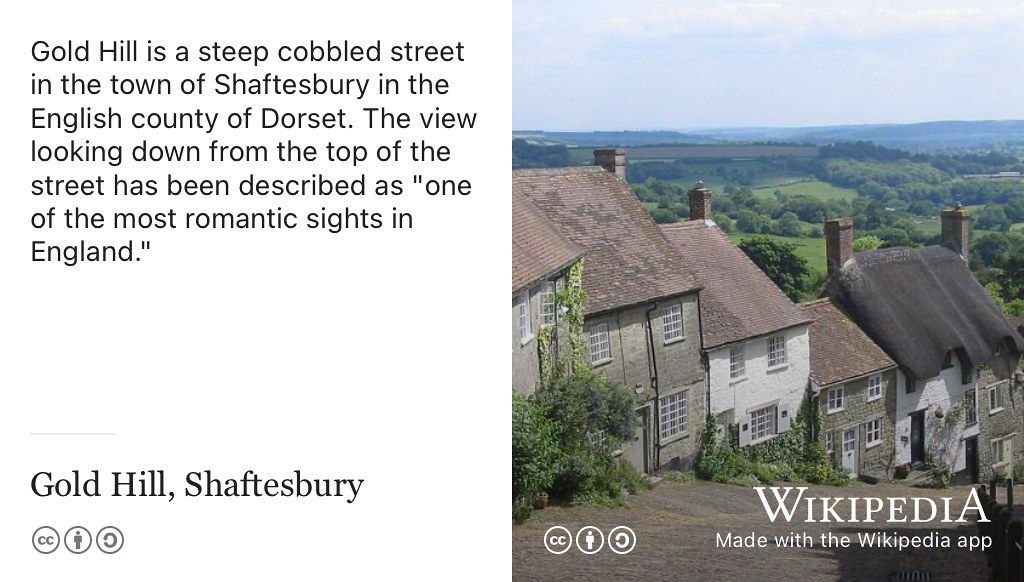
\includegraphics[width=1\linewidth]{images/shaftesbury} 

}

\caption{\href{https://en.wikipedia.org/wiki/Shaftesbury}{Shaftesbury} is the home of \href{https://en.wikipedia.org/wiki/Gold_Hill,_Shaftesbury}{Gold Hill} and \href{https://en.wikipedia.org/wiki/Shaftesbury_School}{Shaftesbury School}. Image of Gold Hill by Sean Davis via Wikimedia Commons \href{https://w.wiki/32gW}{w.wiki/32gw} made with the \href{https://apps.apple.com/us/app/wikipedia/id324715238}{Wikipedia app}.}\label{fig:shaft-fig}
\end{figure}



So thanks Shaftesbury for lessons on top of Gold Hill and the Hovis Advert, one of Britain's best-loved adverts. \citep{hovisadvert} 🍞

\hypertarget{swindon}{%
\subsection{Thank you Swindon}\label{swindon}}

Thanks to headteacher \href{https://www.swindonadvertiser.co.uk/news/14113118.lydiard-school-looking-to-help-others-improve-gcse-results/}{Clive Zimmerman}, his team of staff, Mr M. Carter , Mr K. Thomas and the students of \href{https://en.wikipedia.org/wiki/Lydiard_Park_Academy}{Greendown Community School (now Lydiard Park Academy)} in Swindon, Wiltshire for hosting my second PGCE teaching placement. It was fun teaching you about waves using \href{https://twitter.com/alomshaha}{Alom Shaha}'s jelly babies and kebab sticks shown in figure \ref{fig:shaha-fig}.

\begin{figure}

{\centering 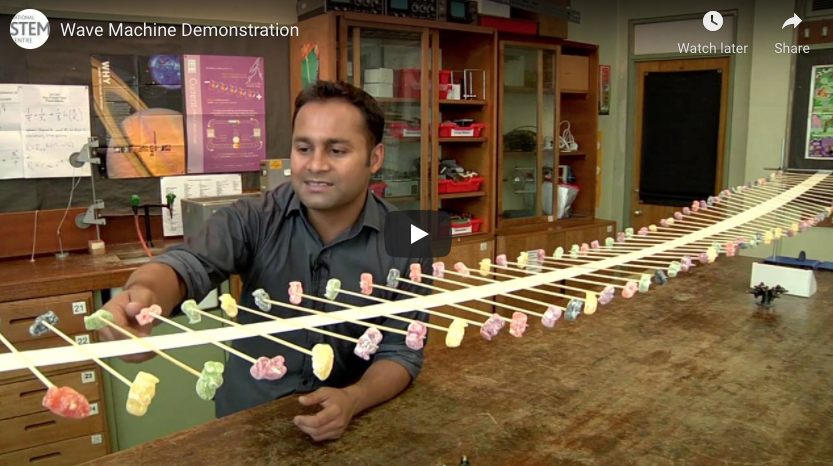
\includegraphics[width=0.99\linewidth]{images/youtube-alom} 

}

\caption{A wave machine demonstration by Alom Shaha with Physics and jelly babies. What's not to like? \citep{youtube-alom}}\label{fig:shaha-fig}
\end{figure}



So thanks Swindon for being \href{https://en.wikipedia.org/wiki/Great_Western_Railway}{great and western} and \href{https://en.wikipedia.org/wiki/Swindon_Town_F.C.}{Swindon Town Football Club}, the best football team in the whole of Wiltshire . 🙏

\hypertarget{productivefailure}{%
\subsection{Thank you schools}\label{productivefailure}}

Thanks to all the schools who interviewed (but rejected me) for my \href{https://en.wikipedia.org/wiki/Newly_qualified_teacher}{Newly Qualified Teacher} (NQT) year. Doing interview lessons, meeting your students and your senior leadership teams was a gruelling but fascinating magical mystery tour of the UK education system, both public and private. Although unsuccessful, these interviews were very productive failures:

\begin{itemize}
\tightlist
\item
  \href{https://en.wikipedia.org/wiki/Writhlington_School}{Wrightlington School}, Radstock, Somerset, see their amazing Orchid project \href{https://wsbeorchids.org/thirty-years-of-the-writhlington-schools-orchid-project-a-teachers-view-by-simon-pugh-jones/}{wsbeorchids.org} run by \href{https://www.bristol.ac.uk/graduation/honorary-degrees/honorary-graduates-2019/simon-pugh-jones/}{Simon Pugh-Jones}
\item
  The \href{https://en.wikipedia.org/wiki/Cooper_School,_Bicester}{Cooper School, Bicester}, Oxfordshire, see their \href{https://www.youtube.com/watch?v=XdywHl2ZA-I}{teacher in my pocket} project
\item
  \href{https://en.wikipedia.org/wiki/St_John\%27s_Marlborough}{St John's Marlborough}, Wiltshire - not to be confused its posher and more famous next door neighbour \href{https://en.wikipedia.org/wiki/Marlborough_College}{Marlborough College}
\item
  \href{https://en.wikipedia.org/wiki/Oasis_Academy_Brislington}{Oasis Academy, Brislington}, Bristol
\item
  \href{https://en.wikipedia.org/wiki/Redland_Green_School}{Redland Green School}, Redland, Bristol
\item
  \href{https://en.wikipedia.org/wiki/The_John_of_Gaunt_School}{The John of Gaunt School}, Trowbridge, Wiltshire
\item
  \href{https://en.wikipedia.org/wiki/Didcot_Girls\%27_School}{Didcot Girls' School}, Didcot, Oxfordshire
\item
  \href{https://en.wikipedia.org/wiki/Cheltenham_Ladies\%27_College}{Cheltenham Ladies' College}, Cheltenham, Gloucestershire\footnote{As a newly trained Jedi knight, freshly armed with a PGCE, I was anxious for my first teaching job and momentarily considered using my pedagogical powers on the ``dark side'' of the force: private education. \citep{nicebutdim} Forgive me for I have sinned!}
\item
  \href{https://en.wikipedia.org/wiki/Blackburn_College_(Blackburn_with_Darwen)}{Blackburn College}, Lancashire ``I read the news today, oh boy! Four thousand holes in Blackburn, Lancashire'' \citep{adayinthelife}
\end{itemize}

So thanks schools, for schooling. 🙏

\hypertarget{stockport}{%
\subsection{Thank you Stockport}\label{stockport}}

Thanks to headteacher Joanne Meredith, her team of staff and the students at \href{https://en.wikipedia.org/wiki/St_Anne\%27s_RC_Voluntary_Academy}{St.~Annes R.C. High School}, Stockport for hosting my \href{https://en.wikipedia.org/wiki/Newly_qualified_teacher}{Newly Qualified Teacher} (NQT) year. Thanks to Keith Doran and other members of the \emph{alternative staff room} for your emotional, moral and practical support throughout the year. According to the \emph{Manchester Evening News}, St.~Anne's is ``the forgotten school'' \citep{stannes1, stannes2}, see figure \ref{fig:st-annes-fig}, but I'll never forget you or the lessons you taught me.

\begin{figure}

{\centering 
\includegraphics[width=1\linewidth]{images/st-annes-rc-high-school} 

}

\caption{Good governance is crucial to good schools. Many schools like St.~Anne's, and the hundreds of children they educate every year, need help from skilled people like you on their governing boards. Why not serve your local community as a ``\href{https://schoolgovernors.thekeysupport.com/governor-training/induction-maintained-school-governors/governance-practice/how-be-critical-friend/}{critical friend}'' on the governing board of a school? Take a look at \href{https://governorsforschools.org.uk/}{governorsforschools.org.uk}. Fair use image via Wikimedia Commons \href{https://w.wiki/33Xs}{w.wiki/33Xs} made with the \href{https://apps.apple.com/us/app/wikipedia/id324715238}{Wikipedia app}}\label{fig:st-annes-fig}
\end{figure}



So thanks Stockport for being Stockport, the magnificent \href{https://en.wikipedia.org/wiki/Stockport_Viaduct}{Stockport Viaduct} and for \href{https://en.wikipedia.org/wiki/Stockport_County_F.C.}{The Hatters}! It's all that matters, Stockport Hatters. 🙏

\hypertarget{moravians}{%
\subsection{Thank you Moravians}\label{moravians}}

Thanks to Thsespal Kundan, Principal of the \href{https://moravianinstitute.com/}{Moravian Institute in Rajpur}, Dehradun, \href{https://en.wikipedia.org/wiki/Uttar_Pradesh}{Uttar Pradesh}, India for hosting me and my friend Doug fresh out of high school on a gap year. We learnt heaps as visiting supply teachers of English and Mathematics, thanks to an introduction from a mutual contact Angus Barker.

\begin{figure}

{\centering 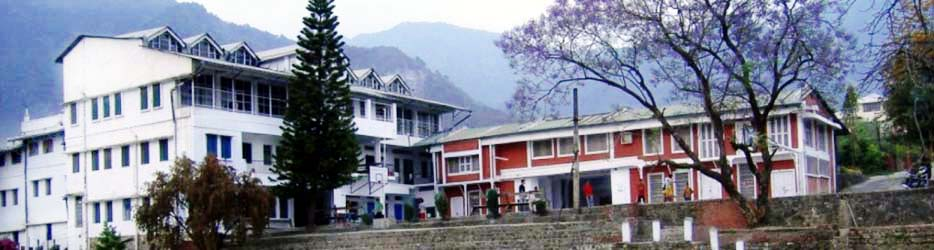
\includegraphics[width=1\linewidth]{images/moravian-insitute} 

}

\caption{The Moravian Institute lies in the foothills of the Himalayas between \href{https://en.wikipedia.org/wiki/Dehradun}{Dehradun} in the \href{https://en.wikipedia.org/wiki/Doon_Valley}{Doon Valley} and the hill station of \href{https://en.wikipedia.org/wiki/Mussoorie}{Mussoorie}. Situated between the \href{https://en.wikipedia.org/wiki/Yamuna}{Yamuna} and \href{https://en.wikipedia.org/wiki/Ganges}{Ganges}, the institute was founded in 1963 by the late Reverend Eliyah Thsetsan Phuntsog of the \href{https://en.wikipedia.org/wiki/Moravian_Church}{Moravian Church} in \href{https://en.wikipedia.org/wiki/Ladakh}{Ladakh}, \href{https://en.wikipedia.org/wiki/Jammu_and_Kashmir_(state)}{Jammu \& Kashmir state} to provide education for \href{https://en.wikipedia.org/wiki/Tibetan_diaspora}{Tibetan refugees} fleeing from their homeland across the Himalayas.}\label{fig:moravian-fig}
\end{figure}



So thanks Moravians (and Angus) for a life changing and formative experience. 🙏

\hypertarget{influences}{%
\subsection{Thank you influencers}\label{influences}}

Some of the most important influences on this guidebook are people I've only met very briefly, virtually or not at all (yet).

\begin{itemize}
\tightlist
\item
  Thanks to \href{https://en.wikipedia.org/wiki/Gayle_Laakmann_McDowell}{Gayle Laakman McDowell} (\href{https://twitter.com/gayle}{@gayle}), for her cracking series of books \citep{techcareer, cracking, crackingpm, crackingthepmcareer} which have been very useful resources both for students I've worked with and me personally
\item
  Thanks to \href{https://yihui.org/en/about/}{Yihui Xie} (\href{https://github.com/yihui}{@yihui}) for \href{https://bookdown.org}{bookdown.org}, the software used to produce this book alongwith the comprehensive and well-written documentation on using it. {[}\citet{xie2017}; \citet{xie2015}; \citet{xie2020};{]}
\item
  Thanks to \href{https://en.wikipedia.org/wiki/Bronnie_Ware}{Bronnie Ware} for her \emph{\href{https://en.wikipedia.org/wiki/The_Top_Five_Regrets_of_the_Dying}{The Top Five Regrets of the Dying}} \citep{regrets} which helped me to re-align my priorities when they were all out of kilter
\item
  Thanks to blokes on the interwebs whose words I've enjoyed reading including Tim Bray at \href{https://www.tbray.org/ongoing/}{ongoing}, Paul Downey at \href{https://blog.whatfettle.com/}{whatfettle.com}, Paul Graham at \href{http://paulgraham.com/}{paulgraham.com}, Peter Norvig at \href{https://norvig.com/}{norvig.com} and Neil Saunders at \href{https://nsaunders.wordpress.com/blog/}{What you're doing is rather desperate}. Your writing is existence proof that engineers and scientists should also be good communicators.
\item
  Thanks to \href{https://twitter.com/SRS_Sophie}{Sophie Milliken} for \emph{From Learner to Earner: A recruitment insider's guide for students wanting to achieve graduate job success} \citep{milliken} which draws useful distinctions between graduate jobs and graduate schemes
\end{itemize}

So, thanks influencers for being influential. 🙏

\hypertarget{github}{%
\subsection{Thank you githubbers}\label{github}}

Thanks to everyone who has contributed via github. I will credit \emph{any} github contributors here, small or large. Even the typos, it all counts. You can easily add yourself to this roll call by correcting my delibreate mitsakes. 😉

Keith Mitchell (\href{https://github.com/apiadventures}{@apiadventures}), Jan Machacek (\href{https://github.com/janm399}{@janm399}), Zee Somji (\href{https://github.com/ezeethg}{@ezeethg}), Tsvetankov (\href{https://github.com/Tsvetankov}{@Tsvetankov}), teobalmos (\href{https://github.com/teobalmos}{@teobalmos})

If you'd like to contribute via github you can:

\begin{itemize}
\tightlist
\item
  raise an issue at \href{https://github.com/dullhunk/cdyf/issues/new}{github.com/dullhunk/cdyf/issues/new}\\
\item
  click on the \texttt{edit\ this\ page} on any page at \href{http://www.cdyf.me}{cdyf.me} which will initiate a pull request
\item
  \texttt{git\ clone\ https://github.com/dullhunk/cdyf.git} the repository to submit pull requests from your setup
\item
  submit a pull request \href{https://github.com/dullhunk/cdyf/pulls}{github.com/dullhunk/cdyf/pulls}
\end{itemize}

So, thanks githubbers for cloning, forking, pulling, adding, committing and pushing. 🙏

\hypertarget{visualthinkery}{%
\subsection{Thank you Bryan}\label{visualthinkery}}

Many of the illustrations for this book have been drawn by the very talented Bryan Mathers \href{https://twitter.com/BryanMMathers/}{@BryanMMathers} shown in figure \ref{fig:selfportrait-fig}.

\begin{figure}

{\centering 
\includegraphics[width=0.75\linewidth]{images/self-portrait} 

}

\caption{\href{https://bryanmmathers.com/self-portrait/}{Bryan Mathers Self portrait} by \href{https://visualthinkery.com/}{Visual Thinkery} is licensed under \href{https://creativecommons.org/licenses/by-nd/4.0/}{CC-BY-ND}}\label{fig:selfportrait-fig}
\end{figure}



Bryan is an artist, visual thinker and entrepreneur, who also happens to have a Bachelors degree in Computer Science from the University of Glasgow. His combined skills in art, science and engineering made him the perfect fit for illustrating this guidebook. You can find out more about Bryan at \href{https://bryanmmathers.com}{bryanmathers.com} and \href{https://visualthinkery.com}{visualthinkery.com}. I'm \emph{sooo} glad we randomly bumped into each other at a conference shown in figure \ref{fig:bumped-fig}.

So, thanks Bryan for your witty illustrations, this book wouldn't be the same without your visual thinkery. 🙏

\hypertarget{friends}{%
\subsection{Thank you friends}\label{friends}}

Thanks to my friends, especially those who I've enjoyed singing, dancing and live music with. I hope we can sing and dance together to live music again before too long.

So, thank you friends for your friendship. 🙏

\hypertarget{family}{%
\subsection{Thank you family}\label{family}}

To my mum, dad, brother, sister, wife, son, μαμά, μπαμπά and extended family: I'm lucky to have been taught by you and that you've always been there when I needed you. 🇬🇷·🇪🇺·🇬🇧

So, thanks to all my family for your unconditional love. Σε αγαπώ παρα πολύ. 🙏

\hypertarget{duncan}{%
\section{About me}\label{duncan}}

Hello, my name is \href{http://www.cs.man.ac.uk/~hulld/}{Duncan Hull} and I wrote this guidebook for undergraduate and postgraduate students as part of my job at the University of Manchester where I'm a lecturer (≈ \href{https://en.wikipedia.org/wiki/Assistant_professor}{Assistant Professor}) in the \href{https://www.cs.manchester.ac.uk/}{Department of Computer Science}.

So what's \emph{my} story? Like many people, my path has been what \href{https://twitter.com/HelenTupper}{Helen Tupper} and Sarah Ellis call a ``squiggly career'' rather than classic linear one. \citep{squiggly} I've been gainfully employed as a paperboy, supermarket cashier, shelf stacker, sausage factory worker, pork pie filler, chef, dogsbody, field assistant, database administrator, deli counter server, consultant, matchday steward, envelope stuffer, high school teacher, postdoc, research scientist, software engineer, lecturer, external examiner, tutor and academic.

I've done a range of voluntary work too, serving as a competition judge, fundraiser, rabble rouser, \href{https://codeclub.org}{code club} \& \href{https://coderdojo.com}{coderdojo} leader, \href{https://www.manchesterdigital.com/}{digital council} member, \href{https://governorsforschools.org.uk/}{school governor}, curator, librarian, beer drinker, \href{https://wiki-loves-scientists.org.uk/}{wikipedia trainer}, \href{https://sigcse.cs.manchester.ac.uk/}{journal clubber} and editor. But as Ronnie Lane and Ronnie Wood once said:

\begin{quote}
``I wish that I knew what I know now, when I was younger.'' ---Ronnie Lane \citep{faces}
\end{quote}

This guidebook documents some of what I know now, that I wish I'd known, when I was younger. If you're starting your career, I hope you find these insights useful. I've sat on both sides of the interview table, as interviewer and interviewee. I have had some spectacular failures, alongside some modest successes, and have included personal stories where they are relevant.

Most of what I have learned about employment comes from listening to, and watching students interact with employers as they take the first tentative steps in their careers. I've documented some of what they taught me, so reading this book may help you learn from some of their successes and failures.

\hypertarget{legal}{%
\section{Legal stuff}\label{legal}}

I am not a lawyer (\href{https://en.wikipedia.org/wiki/IANAL}{IANAL}) but any opinions expressed in this guidebook are my own and not representative of my current employer, the University of Manchester and therefore do not represent University policy. Also:

\hypertarget{license}{%
\subsection{Licensing}\label{license}}

This guidebook is published under the \href{https://creativecommons.org/licenses/by-nc-nd/3.0/}{Creative Commons Attribution-NonCommercial-NoDerivs 3.0 License} (CC-BY-NC-ND) license. This means you can copy and redistribute the written material provided that:

\begin{itemize}
\tightlist
\item
  You provide full attribution by linking directly to the original source
\item
  You do not use the material for commercial purposes
\item
  You do not make any derivative works
\end{itemize}

See the \href{https://creativecommons.org/licenses/by-nc-nd/3.0/}{full license} (CC-BY-NC-ND) for details.

Images in this guidebook are published under different licenses, depending on the source. For example, Bryan Mathers illustrations are licensed CC-BY-ND, others are different. Each figure caption gives details.

\hypertarget{privacy}{%
\subsection{Your privacy}\label{privacy}}

This site is hosted on \href{https://www.netlify.com/}{netlify.com}, see the \href{https://www.netlify.com/privacy/}{netlify privacy policy}. This site also uses \href{https://docs.netlify.com/monitor-sites/analytics/}{netlify analytics} to monitor website use which complies with the General Data Protection Regulation (GDPR).

Some of these services use cookies. These can be disabled in your browser, see \href{https://www.allaboutcookies.org/manage-cookies/}{allaboutcookies.org/manage-cookies}

So now that we've dispensed with the formalities, let's look at why should you bother reading this guidebook in the first place.

\hypertarget{part-designing-your-future}{%
\part{DESIGNING YOUR FUTURE}\label{part-designing-your-future}}

\hypertarget{bothering}{%
\chapter{Investigating your future}\label{bothering}}

The first half of this book is about designing your future. So before we get started, let's tackle a fundamental design issue. Why the hell would you want to bother investigating your future? Why should you bother with reading this pesky guidebook when you have so many other things on your plate right now:

\begin{itemize}
\tightlist
\item
  You are a busy person, YES! ☑️
\item
  Your time is a precious and finite resource, YES! ☑️
\item
  You could be spending that precious time right now in lots of other ways, YES! ☑️
\item
  There are mountains of self-help guides and courses already, YES! ☑️
\item
  Do you really need \emph{yet another} guidebook? YES! ☑️
\end{itemize}

You need this guidebook because it is different to all the other guidebooks! It will help you design, test, build, code and debug your future in computing. Come with me down the rabbit-hole in Figure \ref{fig:rabbit-fig} and let me explain\ldots{} 🐇

\begin{figure}

{\centering \includegraphics[width=0.7\linewidth]{images/Rabbit-hole} 

}

\caption{Shall we go down the rabbit hole? \href{https://bryanmmathers.com/rabbit-hole-learning/}{Rabbit Hole learning} by \href{https://visualthinkery.com}{Visual Thinkery} is licensed under \href{https://creativecommons.org/licenses/by-nd/4.0/}{CC-BY-ND}}\label{fig:rabbit-fig}
\end{figure}



\hypertarget{ilo1}{%
\section{What you will learn}\label{ilo1}}

After reading this chapter you will be able to:

\begin{itemize}
\tightlist
\item
  Identify and decide which parts of this book you are going to read
\item
  Set your expectations for using this guidebook
\item
  Travel down the rabbit hole into the underworld of work
\end{itemize}

\hypertarget{wonderland}{%
\section{Let's go down the rabbit hole}\label{wonderland}}

In the novel \emph{\href{https://en.wikipedia.org/wiki/Alice\%27s_Adventures_in_Wonderland}{Alice's Adventures in Wonderland}} \citep{wonderland}, the heroine Alice follows a \href{https://en.wikipedia.org/wiki/White_Rabbit}{white rabbit} down a hole. What she discovers is a strange underground world populated by weird and wonderful characters. The world of work can sometimes be a mysterious underworld where you adventure in wonderland accompanied by colourful characters.

You will spend lots of time in this wonderland, potentially as much as 80,000 hours of your life. \citep{iip1, iip2} So join me down the rabbit hole, it's fun (honest), and sooner or later you'll have come down here anyway.

\hypertarget{responsibility}{%
\section{Your future is your responsibility}\label{responsibility}}

When \href{https://en.wikipedia.org/wiki/Andy_Stanford-Clark}{Andy Stanford-Clark} started working at IBM, fresh out of University, his boss gave him the following advice:

\begin{quote}
``Nobody cares about your career except you.'' ---Anon \citep{andystanfordclark}
\end{quote}

Andy is now Master Inventor and Chief Technology Officer (CTO) at IBM in the UK so it was probably good advice. Another, slightly more positive way of putting the advice is, the person who cares \emph{most} about your career is you. So while there are people who can help design and build your future, ultimately it is \textbf{YOU} who has to take responsibility for the implementation (if you like, the code). The sooner you get coding the better.

At University, there are lots of people can help design and build your future: peers, academic staff, friends, your careers service, employers and your wider network but ultimately it is \emph{your} responsibility to sort out whatever comes next. That might sound obvious but don't wait for somebody else to do it for you, because it probably won't happen.

\hypertarget{entitled}{%
\section{Your degree is not enough}\label{entitled}}

You've worked incredibly hard to get the grades you needed to get into University. You've spent (or are spending) a significant amount of time and money studying whatever it is you are studying at University.

Under these circumstances, you might be tempted to believe that the world owes you something in return for your hard work. Unfortunately that's not the case.

At some point during or after your study, you might find yourself applying for a graduate job or graduate scheme. EVERYONE applying for these opportunities will have a degree or be rapidly on their way to getting one. So having a degree isn't going to set you apart much from your competition. Even having a first class degree \citep{gradeinflation, firstclass} may not distinguish you that much your competitors. Some employers would rather not know (or don't care) what University you went to, so your education might not make you stand out as much as you might like anyway. \citep{bigfour}

What \textbf{will} distinguish you from your competitors will be your \href{experiencing.html}{experience}, your projects, your \href{communicating.html}{communication skills} and any awards or honours you might have picked up along the way. If you think that your degree will be enough to get you the job you want, bear in mind that:

\begin{enumerate}
\def\labelenumi{\arabic{enumi}.}
\tightlist
\item
  There are more and more graduates, the UK for example recently passed the milestone of 50\% of young people going into higher education. This compares to just 15\% of over 18s who stayed in higher education in 1980 \citep{lotsofgrads}
\item
  The increase in the number of graduate schemes and graduate jobs has not kept pace with this growth in graduates which means that each graduate job or graduate scheme has more and more graduates applying for it
\item
  There are lots of graduates in your discipline, for example around 9,000 every year in Computer Science alone in the UK. What makes you different from the other 8,999 computer scientists graduating in your year?
\end{enumerate}

\begin{figure}

{\centering 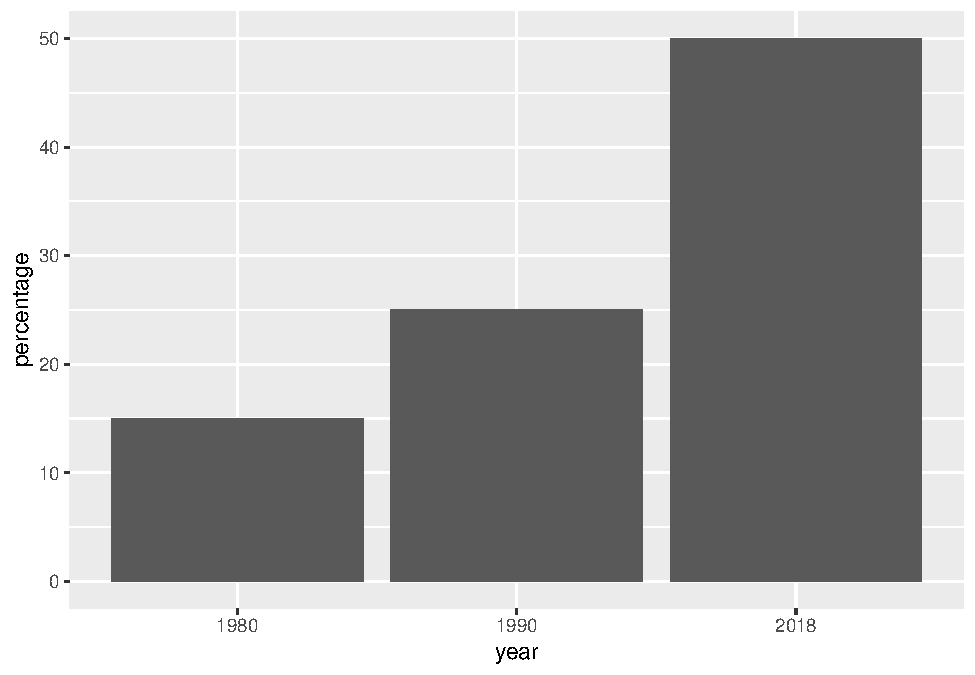
\includegraphics[width=1\linewidth]{cdyf_files/figure-latex/lotsofgrads-fig-1} 

}

\caption{Percentage of young people in the UK going into higher education between 1980 and 2018. Over the last forty years, the proportion of young people going into higher education has more than doubled from 15\% in 1980 to over 50\% in 2018. Data taken from BBC news article on \href{https://www.bbc.co.uk/news/education-49841620}{the symbolic target of 50\% at university reached} \citep{lotsofgrads}}\label{fig:lotsofgrads-fig}
\end{figure}



\begin{quote}
Computing is one of the largest subject areas in UK higher education, and is taught in almost every institution, graduating around 9,000 students every year --Sally Fincher \citep{fincherreview}
\end{quote}

Now, don't be disillusioned by the statistics because a degree can open doors to many careers in computing. What the data in Figure \ref{fig:lotsofgrads-fig} show is that you'll need to look beyond your formal education to distinguish yourself from your competition. Your degree can certainly help you start a career, but it is typically not enough by itself.

\hypertarget{roi}{%
\section{Maximising your future}\label{roi}}

Studying at University is a significant investment of your time and money. Hopefully, you've picked a subject that stimulates and challenges you intellectually while allowing you to find and develop your unique talents. But there's another reason that you probably chose to study at University and that was to improve your job prospects. This guidebook will:

\begin{enumerate}
\def\labelenumi{\arabic{enumi}.}
\tightlist
\item
  Help you maximise the return on the substantial investment of time and money (\href{https://en.wikipedia.org/wiki/Return_on_investment}{ROI}) you've put into your study
\item
  Give you an overview of important professional issues that are sometimes neglected or sidelined in University curricula
\item
  Highlight and review essential resources beyond this guidebook that will help with the above
\end{enumerate}

All of the resources that can help you are scattered around in lots of different places. There are books, there are videos, there are podcasts, there are websites and jobs boards. There are online courses, blogs, social media, newspaper columns, journal articles, marketing material and many other good resources. It is overwhelming.

\hypertarget{thisstuffmatters}{%
\section{Too late when you graduate}\label{thisstuffmatters}}

You might be tempted to postpone making difficult career decisions. I'll do it tomorrow. I'll do it next week. I'll do it next year. I'll finish this assignment. I'll finish this exam. I'll finish this semester. Procrastination is a part of the human condition \citep{procrastination}:

\begin{quote}
``I'll get my degree out of the way first then worry about jobs and careers when I finish University'' --Pro Crastinator
\end{quote}

It probably doesn't help that many of issues described and discussed in this book are typically not closely integrated into the curriculum in Higher Education. You'll often find them on the edges, or completely outside of, standard University curricula. Broadly speaking, the professional issues described in this book are usually covered by pastoral support systems, counselling services, careers services, trade organisations, professional bodies, student unions and their societies,.

Despite being sidelined, these issues matter and it is in your own selfish interests to start thinking about them right now. According to recent estimates by \emph{Investors in People}, the average person spends \textbf{80,000 hours} working during their lifetime. \citep{iip2} So, \emph{whatever} you end up doing after University, you'll be spending a lot of time doing it. Difficult decisions often get sidelined but it is never too early to start thinking about them and doing something. The sooner you start thinking about them the better decisions you'll make about what comes next. It's too late when you graduate.

That doesn't mean you have to know EXACTLY what you want to do when you finish. Lots of students don't and I certainly didn't when I graduated. I'd done a gap year teaching in India, two summer internships (in Sweden and the United States) and a year-in-industry in the UK and I \emph{still} graduated with \textbf{no clue} as to what I wanted to do next! The important thing is that you make a start, and sometimes knowing what you \textbf{don't} want to do is just as valuable as knowing what you do.

Computer scientists call this problem ``search space reduction'', \citep{searchspace} because you have a \href{https://en.wikipedia.org/wiki/Feasible_region}{feasible region} of future possibilities and you need to narrow down the candidates. You could think of coding your future as an \href{https://en.wikipedia.org/wiki/Optimization_problem}{optimisation problem}. Start optimising now because it's too late when you graduate. 🎓

\hypertarget{exams}{%
\section{Yes, this WILL be on the exam}\label{exams}}

Students love to ask their teachers ``\emph{will this be on the exam}''? The short answer is \textbf{YES} (and \textbf{NO})! Yes, this will be on the exam, but NO the exam won't be set by your University. Unlike other courses you've done, the examinations for this course aren't set by your University but by employers. Roughly speaking, there are three kinds of examinations that you'll need to get good at, shown in Table \ref{tab:examtable}

\begin{longtable}[]{@{}lll@{}}
\caption{\label{tab:examtable} Examining your future: The ``exams'' used by employers, what gets assessed and the grades you can get}\tabularnewline
\toprule
\begin{minipage}[b]{(\columnwidth - 2\tabcolsep) * \real{0.28}}\raggedright
Examination\strut
\end{minipage} & \begin{minipage}[b]{(\columnwidth - 2\tabcolsep) * \real{0.58}}\raggedright
What examiners are assessing\strut
\end{minipage} & \begin{minipage}[b]{(\columnwidth - 2\tabcolsep) * \real{0.14}}\raggedright
Grade\strut
\end{minipage}\tabularnewline
\midrule
\endfirsthead
\toprule
\begin{minipage}[b]{(\columnwidth - 2\tabcolsep) * \real{0.28}}\raggedright
Examination\strut
\end{minipage} & \begin{minipage}[b]{(\columnwidth - 2\tabcolsep) * \real{0.58}}\raggedright
What examiners are assessing\strut
\end{minipage} & \begin{minipage}[b]{(\columnwidth - 2\tabcolsep) * \real{0.14}}\raggedright
Grade\strut
\end{minipage}\tabularnewline
\midrule
\endhead
\begin{minipage}[t]{(\columnwidth - 2\tabcolsep) * \real{0.28}}\raggedright
CV, application form
covering letter\strut
\end{minipage} & \begin{minipage}[t]{(\columnwidth - 2\tabcolsep) * \real{0.58}}\raggedright
\begin{itemize}
\tightlist
\item
  Should we invite you to interview ?
\item
  Can you communicate well in writing?
\end{itemize}\strut
\end{minipage} & \begin{minipage}[t]{(\columnwidth - 2\tabcolsep) * \real{0.14}}\raggedright
pass/fail\strut
\end{minipage}\tabularnewline
\begin{minipage}[t]{(\columnwidth - 2\tabcolsep) * \real{0.28}}\raggedright
Interview\strut
\end{minipage} & \begin{minipage}[t]{(\columnwidth - 2\tabcolsep) * \real{0.58}}\raggedright
\begin{itemize}
\tightlist
\item
  Should we offer you a job?
\item
  Can you communicate well verbally?
\item
  Can you communicate well nonverbally?
\end{itemize}\strut
\end{minipage} & \begin{minipage}[t]{(\columnwidth - 2\tabcolsep) * \real{0.14}}\raggedright
pass/fail\strut
\end{minipage}\tabularnewline
\begin{minipage}[t]{(\columnwidth - 2\tabcolsep) * \real{0.28}}\raggedright
Employee performance\strut
\end{minipage} & \begin{minipage}[t]{(\columnwidth - 2\tabcolsep) * \real{0.58}}\raggedright
\begin{itemize}
\tightlist
\item
  Should we promote you?
\item
  Should we give you a pay rise?
\item
  Should we extend your contract?
\end{itemize}\strut
\end{minipage} & \begin{minipage}[t]{(\columnwidth - 2\tabcolsep) * \real{0.14}}\raggedright
pass/fail\strut
\end{minipage}\tabularnewline
\bottomrule
\end{longtable}

So, \emph{yes}, this will be on the exam, but \emph{no}, the exams are obviously not set, administered, invigilated and marked by academics at your University. The exams are set by employers and the results are \textbf{brutally binary}:

\begin{itemize}
\tightlist
\item
  \textbf{PASS}: you've got the interview, job or promotion or\ldots{}
\item
  \textbf{FAIL}: none of the above. Next!
\end{itemize}

One of the challenging things about employers exams are, they typically do not have the bandwidth to give applicants useful feedback, other than a simple pass or fail. When it comes to job applications software engineer \href{https://en.wikipedia.org/wiki/Gayle_Laakmann_McDowell}{Gayle Laakmann McDowell} calls this the ``black hole''. The gravitational force of employers black holes is so strong that no CV or Resume can escape, we'll say more about this in chapter on \protect\hyperlink{debugging}{debugging your CV}.

\begin{figure}

{\centering \includegraphics[width=1\linewidth]{images/Gimme Some Credit - Sketch} 

}

\caption{\emph{no} this will not be on the exam set by University, but \emph{yes} it will be on the exams set by employers. Some of the most important exams you sit at (and after) University are set by employers. This guidebook will help you prepare for those exams and increase your chances of passing them. Gimme some credit figure by \href{https://visualthinkery.com/}{Visual Thinkery} is licensed under \href{https://creativecommons.org/licenses/by-nd/4.0/}{CC-BY-ND}}\label{fig:exam-fig}
\end{figure}



It's a similar story with interviews, if you fluffed and interview question or came across badly, it can be really difficult to find out from the employer what you did wrong.

\hypertarget{activities}{%
\section{Practicing your future}\label{activities}}

There are practical exercises, for you to get your hands dirty with. Each chapter incorporates activities including individual exercises, group exercises, quizzes and points for wider discussion. Just reading a guidebook won't get you very far, you'll need to do the activities in this book to get the most out of it.

\hypertarget{relatedwork}{%
\section{Navigating your future}\label{relatedwork}}

There are \textbf{lots} of resources out there that offer self-help, career advice and techniques for self-improvement. It can be hard to know where to start, or even how to find your way around the mountains of advice.

\begin{figure}

{\centering \includegraphics[width=1\linewidth]{images/shelfie} 

}

\caption{There are tonnes of resources out there offering advice on the huge range of professional issues. You can't read them all, but this guide will help you navigate the resources that will be most interesting and useful to you}\label{fig:shelfie-fig}
\end{figure}



Lots of professional advice is readily available, but how will you navigate it? This book signposts you to what I think are the most important resources, each chapter has a signposts section, and they are all gathered together in the signpost at the end alongside everything (yes, EVERYTHING!) that this guidebook cites in the \protect\hyperlink{references}{References}.

\hypertarget{joinus}{%
\section{Crediting your future}\label{joinus}}

Get credit for your contributions. As well as being openly accessible on the web, this book is open source too. What this means is, you can contribute in several ways

\begin{itemize}
\tightlist
\item
  View the entire book source on github at \href{https://github.com/dullhunk/cdyf}{github.com/dullhunk/cdyf}
\item
  Click the \textbf{Edit this page}, which appears on the right hand side of every chapter with the \href{https://en.wikipedia.org/wiki/Octocat}{octocat} logo
\item
  Raise an issue \href{https://github.com/dullhunk/cdyf/issues/new}{github.com/dullhunk/cdyf/issues/new}
\item
  Submit a pull request \href{https://github.com/dullhunk/cdyf/pulls}{github.com/dullhunk/cdyf/pulls}, If you're not familiar with pull requests, see \href{http://makeapullrequest.com/}{makeapullrequest.com}
\item
  \href{http://www.cs.man.ac.uk/~hulld/contact.html}{Email me suggestions for improvements} if you don't want to use github
\end{itemize}

Any corrections or suggestions that get included will be fully acknowledged in the \protect\hyperlink{thanks}{acknowledgements}, unless you tell me otherwise. We welcome all improvements, however small.

All the written content for this guidebook is licensed under CC-BY-NC-ND, see the license.

\hypertarget{thinkdifferent}{%
\section{Your future is different}\label{thinkdifferent}}

I wrote this guidebook because I needed a resource for students to help them design, build, test and debug their futures. I wanted a single resource that could help students compete for jobs while at University, or shortly after graduating. I could not find anything suitable that met all the requirements of the students I was teaching. So I wrote this one which contains some new material and recommends the best resources if you want to know more. These are found in the signposts sections of each chapter.

This book aims to combine these perspectives and to be different from existing resources in the following ways:

\hypertarget{signposted}{%
\subsection{Your future is signposted}\label{signposted}}

Some career resources claim (or imply) that they are the \emph{all you will need} to solve a particular problem or worse: solve \emph{all of your problems}! Just buy this book, do this course, watch this video, listen to this podcast and all your problems will go away! Rather than continue this trend, this book \textbf{signposts} some of the most useful resources.

Scientists call this \textbf{citation}, rather than signposting. I've signposted and cited sources in this guidebook so that you can :

\begin{enumerate}
\def\labelenumi{\arabic{enumi}.}
\tightlist
\item
  Check and verify any facts and claims I make in this book for yourself
\item
  Go and consult the original sources if you think they might be useful
\end{enumerate}

While this guidebook cites lots of resources, some of them are more important than others. Each chapter summarises these in a signposts section. You'll find everything else in the \protect\hyperlink{referencing}{references} section. The University of Manchester has physical and electronic copies of many (but sadly not all) of the books listed here.

We're not suggesting that you read \emph{all} these books right now, but that if a particular chapter has piqued your interest, these signposts are good places to keep going, if you haven't already read them. I hope you'll find these signposts handy for navigating the mountains of advice. Not all who wander are lost. 🗺️🧭

\hypertarget{study}{%
\subsection{Guiding your future}\label{study}}

This guidebook to your future accompanies a course that has been co-designed by students for students, with input from academics and employers. It unites several disparate themes into one coherent story, from fundamental questions about identity and wellbeing through to more applied and practical advice on job hunting, career progression and life after University. Resources that do this are typically scattered around in many different places. There is usually no narrative to tie them all together to help students navigate the mountains of advice as embark on the first stages of their careers.

Although this is a course guidebook used in the second year undergraduate teaching, you don't need to be enrolled on the course to benefit from reading it, watching the videos and doing the exercises and coding challenges.

\hypertarget{updates}{%
\subsection{Your future is constantly updated}\label{updates}}

You are reading the alpha version, the \href{https://en.wikipedia.org/wiki/Minimum_viable_product}{Minimum Viable Product} (MVP) of this guidebook. That's software engineer talk for saying it isn't finished yet. Subsequent versions, will be continuously and iteratively released on a daily and weekly basis. They will include:

\begin{itemize}
\tightlist
\item
  More quizzes for better interactivity
\item
  More videos on the \href{https://www.youtube.com/channel/UCLBv_u8JmyUPqmRALIjVnLg}{Coding your Future YouTube channel}
\item
  Audio podcasts in the \href{listening.html}{Coding your Future}
\item
  More illustrations throughout the book
\item
  Improved content, finish incomplete chapters
\item
  Fix bugs and typos
\item
  Your \href{\%7B\#joinus\%7D}{suggestions for improvements and corrections, via github etc}
\end{itemize}

I'm taking a \href{https://en.wikipedia.org/wiki/Release_early,_release_often}{Release Early, Release Often} \citep{Raymond1999} approach to publishing this guidebook, you could call it agile book development. \citep{realagile}

\begin{quote}
Agile: make it up as you go along. Waterfall: make it up before you
start, live with the consequences.

--- Paul Downey (@psd) \href{https://twitter.com/psd/status/568324759521501184}{February 19,
2015}
\end{quote}

\hypertarget{im-deliberately-writing-in-first-person-narrative}{%
\subsection{I'm deliberately writing in first person narrative}\label{im-deliberately-writing-in-first-person-narrative}}

A lot of scientific and technical writing is written in the third person or passive voice, which is fine for academic writing, but can alienate readers. I have opted to use first person narrative where possible as it is shorter, and hopefully more engaging for you to read. \citep{googler} Where relevant, I've told stories to illustrate key points.

\hypertarget{openaccess}{%
\subsection{Your future has no paywall}\label{openaccess}}

You don't need to pay anything to read this book online because its openly available, see the \protect\hyperlink{licensing}{license terms} (CC-BY-NC-ND). Publishing this guidebook online makes it findable and accessible, something that isn't true of lots of knowledge locked up inside other books.

Because this guidebook is online, it is searchable, browsable and linkable. You can link to whatever level you like, top level, chapter level and to every section and subsection level. Everything important has a Uniform Resource Locator (\href{https://en.wikipedia.org/wiki/URL}{URL}).

\hypertarget{av}{%
\subsection{Your future has audio \& video}\label{av}}

This book is not just words and pictures, but includes audio and video as well, especially:

\begin{enumerate}
\def\labelenumi{\arabic{enumi}.}
\tightlist
\item
  videos produced by third parties that are worth watching
\item
  audio produced by third parties that are worth listening to, either individual episodes or whole series
\item
  short videos produced by me, which augment the written content of this book, see the \href{https://www.youtube.com/channel/UCLBv_u8JmyUPqmRALIjVnLg}{Coding your Future YouTube channel}
\item
  the coding your future podcast which interviews undergraduate students
\end{enumerate}

\hypertarget{engaging-your-future}{%
\section{Engaging your future}\label{engaging-your-future}}

I've tried to make the content of this book as engaging as possible by including pictures and conversations. \emph{Your future} is deliberately playful and light-hearted. If you think it can be improved, \protect\hyperlink{joinus}{let me know}. I always welcome constructive feedback, especially when it comes via a pull request.

\begin{quote}
Let's go Captain
\href{https://t.co/LN33dh5dip}{pic.twitter.com/LN33dh5dip}

--- VeraM 🇬🇷🇬🇧🇪🇺 (@FonikhSoupia) \href{https://twitter.com/FonikhSoupia/status/1285742247711997954}{July 22,
2020}
\end{quote}

\hypertarget{sign1}{%
\section{Signposting your future}\label{sign1}}

Each chapter in this book has a signposts section, highlighting key reading, watching or listening you could do next. This chapter has addressed the question of \textbf{why should you bother coding your future}? The answer is that your future is your responsibility and no-one elses. There are lots of people can help shape your future, but none more than yourself. Software engineer \href{https://en.wikipedia.org/wiki/Robert_C._Martin}{Robert C. Martin} argues this point in his book \emph{The Clean Coder: A Code of Conduct for Professional Programmers}. \citep{cleancoder}

What's good about \emph{The Clean Coder} is that it is short (only 200 pages), well written and to the point. The main part of the book covers professional issues in software engineering, some of which I discuss in \href{surviving.html}{surviving your future}, so \emph{The Clean Coder} is an essential signpost for chapter 10 as well.

\hypertarget{tldr1}{%
\section{Summarising your future}\label{tldr1}}

If all that was \href{https://en.wiktionary.org/wiki/too_long;_didn\%27t_read}{too long, didn't read} (TL;DR) for you, then you'll be relieved to hear that each chapter (including this one) has a TL;DR summary.

\begin{figure}

{\centering 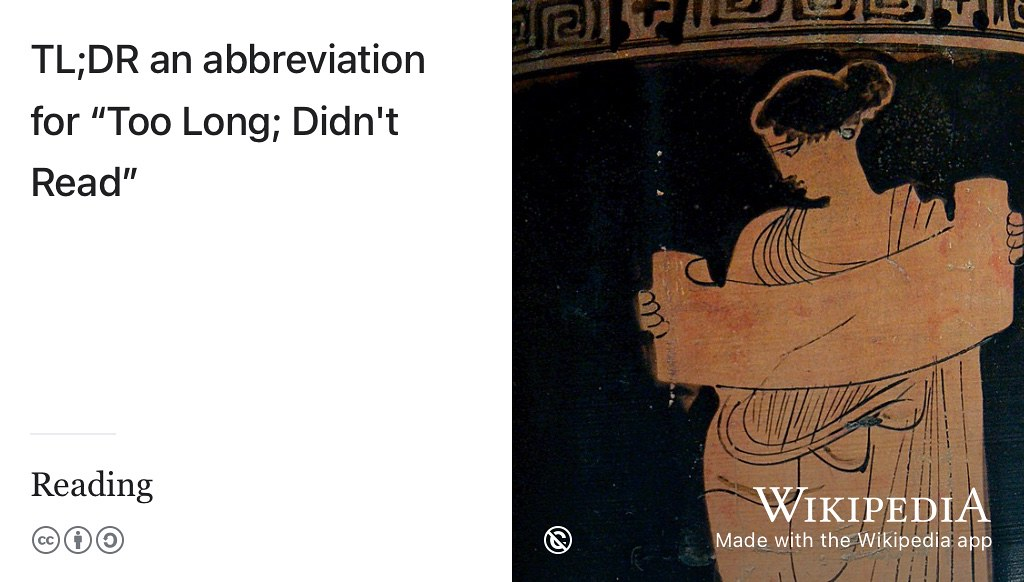
\includegraphics[width=1\linewidth]{images/TLDR} 

}

\caption{Too long, didn't read? \href{https://bryanmmathers.com/tldr/}{TL;DR} by \href{https://visualthinkery.com/}{Visual Thinkery} is licensed under \href{https://creativecommons.org/licenses/by-nd/4.0/}{CC-BY-ND}}\label{fig:tldr-fig}
\end{figure}



The TL;DR for this chapter is, you should read this guidebook because it will help you design, build, test, debug and code your future in computing.

\hypertarget{knowing}{%
\chapter{Knowing your future}\label{knowing}}

Hello, who are you? What's your story? What are you good at, what do you like doing and what do you value? What are your hopes and dreams for the future? Tell me about your education and who you are. What unique talents are you finding and developing during your education? How are you striving to become the best possible version of you? Knowing your possible futures depends on knowing who you are now. 🏆

\begin{figure}

{\centering \includegraphics[width=1\linewidth]{images/goal of education} 

}

\caption{Your education is a crucial part of your story and who you are. The purpose of your education is not just to get you a job but to find and develop your unique talents. What are you unique talents? How are you developing them? \href{https://www.flickr.com/photos/122135325@N06/16627558943/}{Goal of Education} sketch by \href{https://visualthinkery.com/}{Visual Thinkery} is licensed under \href{https://creativecommons.org/licenses/by-nd/4.0/}{CC-BY-ND}}\label{fig:goal-fig}
\end{figure}



\hypertarget{ilo2}{%
\section{What you will learn}\label{ilo2}}

Reading this chapter and doing the activities will help you to

\begin{itemize}
\tightlist
\item
  Improve your self-awareness, knowing yourself better will help you to know your future more clearly
\item
  Describe what you know: what is in your \textbf{head},
\item
  Describe what have you done: (\textbf{hands})
\item
  outlining some of your values: what is in your \textbf{heart}
\item
  Identify your protected characteristics
\item
  Check and be grateful for any privileges that you may have
\end{itemize}

\hypertarget{story}{%
\section{What's your story, coding glory?}\label{story}}

\begin{quote}
``If you are human, you love stories. Why? We're hardwired to love stories because they help us understand
our world and are essential to our evolution. We use stories to organise and communicate our surroundings
and our past, present and future'' ---Heather Box and Julian Mocine-McQueen \citep{freeyourstory}
\end{quote}

Self-awareness, understanding who you are, is important for leading a healthy and happy life, and likely to be an important factor in your future success. One way to develop self-awareness is to think about what your story is. \citep{freeyourstory} How did you get here, where are you going, what has inspired you? Who is the authentic you? \citep{regrets} What are your hopes and dreams? By starting to answer these questions you will gain a better understanding of who you are. This includes strengths, weaknesses, motivation and values. \citep{parachute2020}

Universities offer many opportunities for self improvement, self discovery and developing your unique skills. One way to build your self-awareness is to reflect on your knowledge, values and skills. In Waldorf education this is characterised as ``head, heart and hands''. \citep{headhearthands}

\begin{enumerate}
\def\labelenumi{\arabic{enumi}.}
\tightlist
\item
  \textbf{Head}: What do you \emph{know}?
\item
  \textbf{Heart}: What do you \emph{value}, what motivates you?
\item
  \textbf{Hands}: What can you \emph{do}? What have you \emph{done} so far? What will you do in the future?
\end{enumerate}

Answering these questions will help you understand your story.

\hypertarget{no42}{%
\section{Ikigai: What is the meaning of life?}\label{no42}}

Many of the learning outcomes described above are non-trivial. You may have good self-awareness and be able to describe aspects of who you are in a matter of minutes. Other personality traits make take longer to realise. You can develop better self-awareness by describing four attributes shown in Figure \ref{fig:iki-fig}, together these are known as your ikigai (生き甲斐) or ``reason for being''.

\begin{itemize}
\tightlist
\item
  what do you love doing?
\item
  what are you good at?
\item
  what does the world need?
\item
  what can you be paid for?
\end{itemize}

\begin{figure}

{\centering \includegraphics[width=0.8\linewidth]{images/ikigai} 

}

\caption{Reasons for being, a concept in Japanese known as ``ikigai''. Image by Emmy van Deurzen on Wikimedia Commons. According to ikigai, a meaningful life combines doing four things. 1. What you are good at 2. What you love 3. What the world needs and 4. What you can get paid for. Illustration by Nimbosa derived from works in the public domain by Dennis Bodor and Emmy van Deurzen, CC BY-SA 4.0 on Wikimedia Commons \href{https://w.wiki/qWT}{w.wiki/qWT}}\label{fig:iki-fig}
\end{figure}



You'll be lucky if you can find activities at the intersection of all four sets shown Figure \ref{fig:iki-fig}. In practice, you may realistically only be able to achieve one, two or three. That said, it's still a valuable exercise to think about what is in each category for you.

\hypertarget{self-assess-your-ikigai}{%
\section{Self assess your ikigai}\label{self-assess-your-ikigai}}

Take a sheet of paper, draw the four overlapping rings shown in Figure \ref{fig:iki-fig}, and spend five to ten minutes adding things in each ring.

\begin{itemize}
\tightlist
\item
  What are your values?
\item
  What motivates you?
\item
  Are there things you like doing that you aren't particularly good at?
\item
  Why does that make them enjoyable?
\end{itemize}

\begin{figure}

{\centering \includegraphics[width=0.5\linewidth]{images/Know who you are} 

}

\caption{How well do you know yourself. Know who you are sketch by \href{https://visualthinkery.com}{Visual Thinkery} is licensed under \href{https://creativecommons.org/licenses/by-nd/4.0/}{CC-BY-ND}}\label{fig:know-fig}
\end{figure}



Thinking about your ikigai will clarify your knowledge of yourself. Some parts of your identity are so important that they are protected by legislation, in the UK and in other countries. The next section looks at those.

\hypertarget{protected}{%
\section{Your protected characteristics}\label{protected}}

Some of your characteristics are protected. The Equality Act of 2010\footnote{\url{http://www.legislation.gov.uk/ukpga/2010/15/contents}} protects you from discrimination at work or in education, based on what are known as ``protected characteristics''. \citep{equality}. This means that:

\begin{itemize}
\tightlist
\item
  Your \textbf{age} should not determine how you are treated
\item
  Your \textbf{disabilities} should not determine how you are treated
\item
  Your \textbf{gender} should not determine how you are treated \citep{inferior, damore, damoreguardian, everydaysexism}
\item
  Your \textbf{gender re-assignment} should not determine how you are treated
\item
  Your \textbf{marriage} or civil partnership should not determine how you are treated
\item
  Your \textbf{pregnancy} and maternity should not determine how you are treated
\item
  Your \textbf{race} (including colour, nationality, ethnic or national origin) should not determine how you are treated \citep{nottalking, superior}
\item
  Your \textbf{religion} or beliefs should not determine how you are treated
\item
  Your \textbf{sex} should not determine how you are treated \citep{harassment}
\item
  Your \textbf{sexual orientation} should not determine how you are treated \citep{nosex}
\end{itemize}

\hypertarget{goals}{%
\section{Coding challenges}\label{goals}}

This chapter has looked at some big issues around identity, by inviting you to think about some fundamental questions. Another way to think about these questions is as coding challenges. They are non-trivial questions to answer, it might take you weeks, months or even years to answer some of them. But they are worth spending time thinking about

\begin{itemize}
\tightlist
\item
  What are your values?
\item
  What makes you happy?
\item
  What do you want to get from your time at University?
\item
  What do you want after University?
\item
  Where do you see yourself in \emph{x} years time?
\end{itemize}

The signposts in the next section may help tackle some of these coding challenges.

\hypertarget{sign2}{%
\section{Signposts from here on identity}\label{sign2}}

This chapter challenges you to reflect on who you are and what you're good at. We've only scratched the surface, so if you want to dig deeper you'll find the following resources useful:

\begin{itemize}
\tightlist
\item
  \emph{The Top Five Regrets of the Dying}
\item
  \emph{What Colour is Your Parachute?}
\item
  \emph{How Your Story Sets You Free}
\item
  A range of books about privilege
\end{itemize}

\hypertarget{regret}{%
\subsection{Your dying regrets?}\label{regret}}

One of \emph{\href{https://en.wikipedia.org/wiki/The_Top_Five_Regrets_of_the_Dying}{The Top Five Regrets of the Dying}} \citep{regrets} is that people wish they'd had the courage to live a life true to themselves, and not a life that others expected of them. Figuring out exactly who your authentic self is can be challenging. \href{https://en.wikipedia.org/wiki/Bronnie_Ware}{Bronnie Ware's} book might help, it has some very moving, personal and insightful true stories of peoples regrets that will illuminate your own values and might just change your life. The top five regrets, outlined in the book are:

\begin{enumerate}
\def\labelenumi{\arabic{enumi}.}
\tightlist
\item
  I wish I'd had the courage to live a life true to myself, not the life others expected of me
\item
  I wish I hadn't worked so hard
\item
  I wish I'd had the courage to express my feelings
\item
  I wish I had stayed in touch with my friends
\item
  I wish that I had let myself be happier
\end{enumerate}

You need to be courageous to live a regret-free life but the alternative is to die full of regret, see Bronnie's video in figure \ref{fig:bronnie-fig}.

\begin{figure}

{\centering 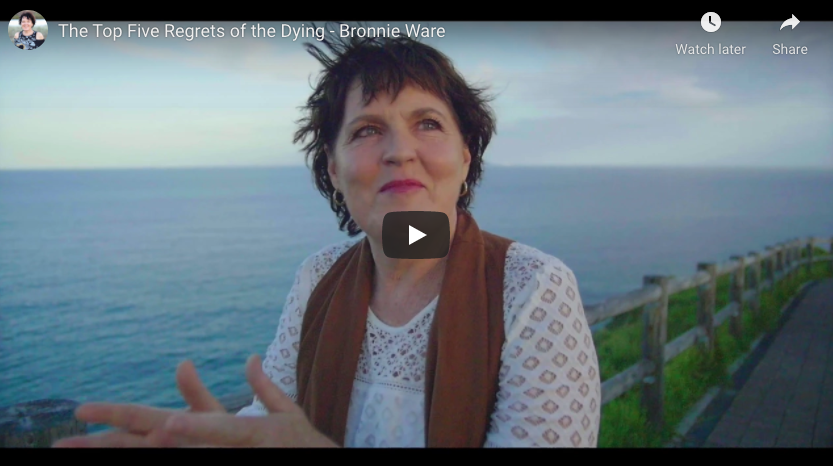
\includegraphics[width=0.99\linewidth]{images/youtube-bronnie} 

}

\caption{Palliative care nurse Bronnie Ware explains the top five regrets of the dying. [@youtube-bronnie] Bronnie learned a lot from looking after people on their deathbeds, then wrote it all down in a fantastic book [@regrets].}\label{fig:bronnie-fig}
\end{figure}

\hypertarget{parachute}{%
\subsection{Colouring your parachute}\label{parachute}}

Since first being published in 1972, over ten million copies of \emph{\href{https://en.wikipedia.org/wiki/What_Color_is_Your_Parachute\%3F}{What Colour is Your Parachute?}} have been sold. It has been translated into 20 languages and is used in 26 countries. What is good about \emph{Parachute} is that it has some useful \emph{self-inventory} exercises that go beyond the introductory ones in this guidebook, particularly in the context of your future career. While the style and examples can be U.S. centric, it's a classic self-help book that looks at a broad variety of issues around job hunting. The author, \href{https://en.wikipedia.org/wiki/Richard_Nelson_Bolles}{Richard Nelson Bolles} was a Harvard educated chemical engineer and he explains how you can't possibly decide what to do in five years time in the video in figure \ref{fig:bolles-fig}. Where do you see yourself in five years time? is a question some interviewers like to ask.

\begin{figure}

{\centering 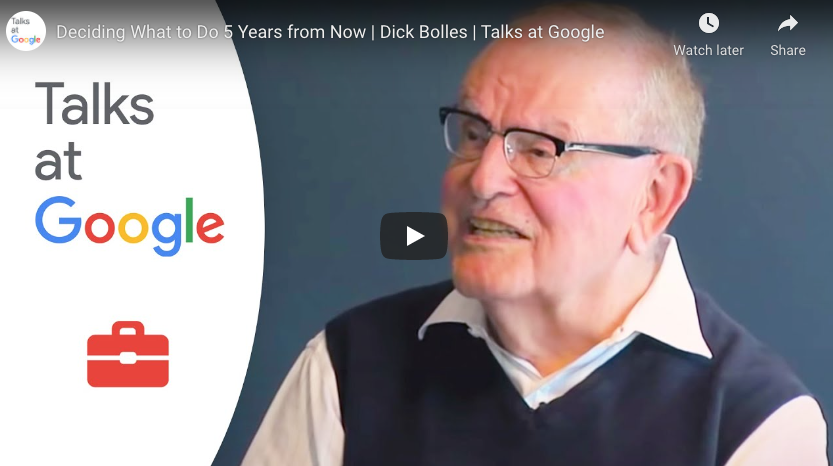
\includegraphics[width=0.99\linewidth]{images/youtube-bolles} 

}

\caption{Where will you be five years from now? Best-selling author Dick Bolles talks at the Googleplex about the gaps between education and employment. [@youtube-bolles]}\label{fig:bolles-fig}
\end{figure}

\hypertarget{whats-your-story}{%
\subsection{What's your story?}\label{whats-your-story}}

A useful technique for developing self-awareness is to think about what your story is. Heather Box and Julian Mocine-McQueen's book \emph{How Your Story Sets You Free} \citep{freeyourstory} takes a storytelling approach to help you gain a better picture of who you are and what you value. What's good about this book is its short, less than 100 pages and contains practical exercises which extend those in this chapter.

\hypertarget{check-your-privileges}{%
\subsection{Check your privileges}\label{check-your-privileges}}

Reflecting on your identity should lead you to check any privileges you might have. Being grateful for any privileges you may have is also beneficial for your mental health which we talk about in the chapter on \protect\hyperlink{wellbeing}{your well-being} So:

\begin{itemize}
\tightlist
\item
  \textbf{If you're white} a good place to start understanding your white privileges is \emph{\href{https://en.wikipedia.org/wiki/Why_I'm_No_Longer_Talking_to_White_People_About_Race}{Why I'm No Longer Talking to White People About Race}} by \href{https://en.wikipedia.org/wiki/Reni_Eddo-Lodge}{Reni Eddo Lodge} \citep{nottalking} and \emph{\href{https://en.wikipedia.org/wiki/Superior:_The_Return_of_Race_Science}{Superior: The Return of Race Science}} by \href{https://en.wikipedia.org/wiki/Angela_Saini}{Angela Saini}
\item
  \textbf{If you're male} a good place to start understanding the privileges you have as a result of being a man is \emph{\href{https://en.wikipedia.org/wiki/Inferior_(book)}{Inferior}} by \href{https://en.wikipedia.org/wiki/Angela_Saini}{Angela Saini} \citep{inferior}
\item
  \textbf{If you're socially privileged} a good place to start understanding the privileges you have as a result of your class is \emph{The Class Ceiling: Why it Pays to be Privileged} by Sam Friedman and Daniel Laurison \citep{classceiling}. If you were privately educated in Britain (or elsewhere) you should read \emph{\href{https://en.wikipedia.org/wiki/Engines_of_Privilege}{Engines of Privilege: Britain's Private School Problem}} \citep{nicebutdim}
\item
  \textbf{If you're heterosexual} a good place to start understanding the privileges you have as a result of your sexual orientation is \href{https://en.wikipedia.org/wiki/Ben_Britton}{Ben Britton}'s presentation on \emph{No sexuality please, we're scientists} \citep{nosex} which covers bisexuality and homosexuality, including lesbian and gay homosexuality
\item
  \textbf{If you're gender binary} a good place to start understanding the privileges you have as a result of being \href{https://en.wikipedia.org/wiki/Gender_binary}{gender binary} is Ben Britton's presentation \citep{nosex} which also covers transgender, genderqueer, non-binary and plus identities
\end{itemize}

There is a lot more to your identity than your race, class, gender and sexual orientation, see \protect\hyperlink{protected}{your protected characteristics}.

\hypertarget{tldr2}{%
\section{Summarising self awareness}\label{tldr2}}

\href{https://en.wiktionary.org/wiki/too_long;_didn\%27t_read}{Too long, didn't read} (TL;DR)? Here's a summary:

This chapter has looked at who you are. Being self aware, understanding your strengths and weaknesses is key to getting what you want from your career. Questions about your identity are non-trivial, hopefully this chapter has started you thinking about who you are, what motivates you and what you want out of life. You need to keep thinking about your identity because some aspects of your identity may be constantly changing.

These are fundamental design questions you'll need to address when you starting building your future. We touched on understanding any privileges you may have as being important for understanding who you are but also in being beneficial for your mental health.

In the next chapter, we'll look at mental health in more detail.

\hypertarget{wellbeing}{%
\chapter{Nurturing your future}\label{wellbeing}}

It doesn't matter if you are a student, an employee or even both at the same time. To be successful at studying or working, you need to take your well-being seriously. By well-being, I mean your health and happiness. Your health isn't just about your physical health but also your mental health and the two are very closely linked. It's all too easy when you are busy or stressed to neglect your well-being and then \textbf{bad-stuff™} happens. This chapter looks at your well-being, and how you can nurture it. Because nurturing and caring for yourself now will also nurture your future. 😀

\begin{figure}

{\centering \includegraphics[width=1\linewidth]{images/alan-turing-runner} 

}

\caption{\href{https://en.wikipedia.org/wiki/Alan_Turing}{Alan Turing} was an outstanding Computer Scientist, but did you know he was also a respectable athlete too? He ran, cycled and rowed to relieve stress, \citep{kottke} and came close to competing in the Olympics as a runner. This should come as no surprise, the connections between well-being and academic performance are widely documented. Image via Jonathan Swinton's biography \emph{Alan Turing's Manchester}. \citep{manturing} The copyright holder for this image has been unidentifiable or unresponsive at their self-advertised contact details.}\label{fig:turing-fig}
\end{figure}



\hypertarget{ilo3}{%
\section{What you will learn}\label{ilo3}}

By the end of this chapter you will be able to:

\begin{itemize}
\tightlist
\item
  Identify some of the symptoms of mental ill health in yourself and your peers, particularly anxiety and depression
\item
  Describe five self-help techniques for improving mental health
\item
  Describe services and other people you can approach if you (or someone you know) is being affected by mental ill health and self-help isn't enough
\item
  Schedule activities for improving mental and physical health into your daily or weekly routine
\item
  DISCLAIMER: I am neither a medical doctor or a psychologist: If you're affected by mental ill health, you should speak to a trained professional. This chapter just gives you a quick overview of mental health and points you to where you can find out more.
\end{itemize}

\hypertarget{illhealth}{%
\section{Mental ill health}\label{illhealth}}

Stress can lead to many kinds of ill health. Turing was put under lots of stress by his government bosses, people like \href{https://en.wikipedia.org/wiki/Alastair_Denniston}{Alastair Denniston} and \href{https://en.wikipedia.org/wiki/Stewart_Menzies}{Stewart Menzies}. \citep{imitationgame} On describing his work for the government and why he punished himself so much in training, Alan Turing said:

\begin{quote}
``I have such a stressful job that the only way I can get it out of my mind is by running hard; it's the only way I can get some release'' --Alan Turing. \citep{kottke}
\end{quote}

University is a positive experience for many people, however like Alan, you may also experience periods of stress. This may also be accompanied by anxiety, loneliness and depression. Financial, social and academic pressures alongside concerns about employability and an ongoing pandemic of COVID-19 can all have an impact on your wellbeing. Statistically, one in four of us will be affected by mental ill health during our lifetime. Two of the most common forms of mental ill health are:

\begin{itemize}
\tightlist
\item
  \textbf{Anxiety}: \emph{persistent} feelings of unease, such as worry or fear
\item
  \textbf{Depression}: a low mood that \emph{lasts for a long time} and affects your everyday life
\end{itemize}

The \emph{persistent} and \emph{lasting a long time} are important here because while its part of the human condition to worry and feel low, that doesn't \emph{necessarily} mean you are affected by poor mental health.

\hypertarget{anxiety}{%
\subsection{Anxiety}\label{anxiety}}

Anxiety is one of most common mental health disorders and can lead to depression, increased risk of suicide. Generalised Anxiety Disorder (GAD), a common form of anxiety is explained in the video in Figure \ref{fig:anxious-fig} and at \href{https://www.nhs.uk/conditions/generalised-anxiety-disorder/}{nhs.uk/conditions/generalised-anxiety-disorder}. People who are affected by anxiety may struggle to function normally, and find routine everyday task difficult or impossible.

\begin{figure}

{\centering 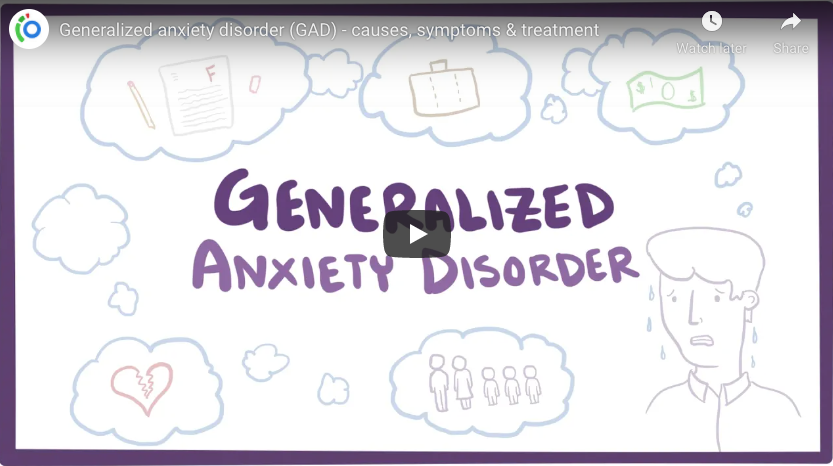
\includegraphics[width=0.99\linewidth]{images/youtube-anxiety} 

}

\caption{Generalised anxiety disorder is a condition characterised by excessive, persistent and unreasonable amounts of anxiety and worry about everyday things. \citep{youtube-anxiety} Note that the video takes an American perspective using American terminology such as \href{https://www.psychiatry.org/psychiatrists/practice/dsm}{DSM--5}.}\label{fig:anxious-fig}
\end{figure}



\hypertarget{depression}{%
\subsection{Depression}\label{depression}}

Millions of people around the world live with depression. If you are affected by depression it can be really hard to talk about it as there are many social stigmas around mental health. Thankfully depression is largely preventable and treatable. Recognising depression and seeking help is the first and most critical step towards recovery. To mark \href{https://en.wikipedia.org/wiki/World_Mental_Health_Day}{World Mental Health Day} writer and illustrator Matthew Johnstone tells the story of how he overcame the ``black dog of depression'' in the video in Figure \ref{fig:sad-fig} made in collaboration with the World Health Organization (WHO).

\begin{figure}

{\centering 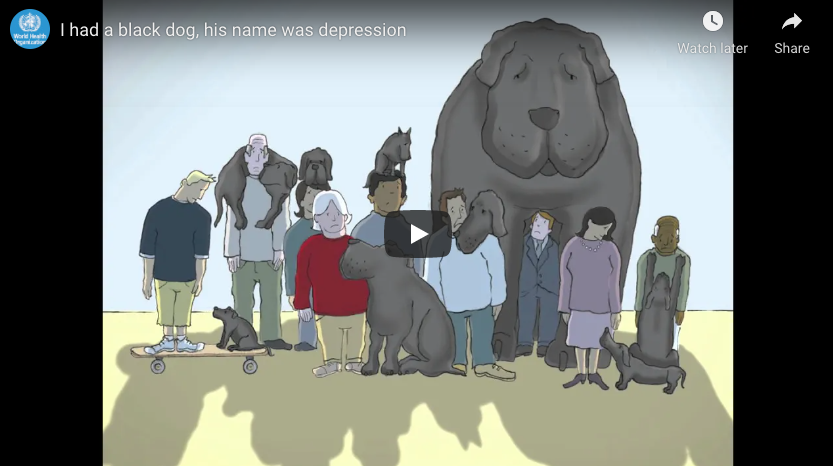
\includegraphics[width=0.99\linewidth]{images/youtube-blackdog} 

}

\caption{Matthew Johnstone explains how he overcame the affects of depression, using the metaphor of the black dog \citep{youtube-blackdog}}\label{fig:sad-fig}
\end{figure}



\hypertarget{drugs}{%
\subsection{Drugs}\label{drugs}}

Prescription medication can help some people with their mental health. For example, when I was affected by depression, \href{https://www.nhs.uk/conditions/ssri-antidepressants/}{Selective Serotonin Reuptake Inhibitors} (SSRIs) worked for me, shown in Figure \ref{fig:citalopram-fig}, but they don't for everybody. Sometimes the drugs don't work, they just make you worse. \citep{drugsdontwork}

\begin{figure}

{\centering 
\includegraphics[width=0.99\linewidth]{images/citalopram} 

}

\caption{\href{https://www.nhs.uk/medicines/citalopram/}{Citalopram} is a type of antidepressant known as a Selective Serotonin Reuptake Inhibitor (SSRI). SSRI's can help some people who have been affected by depression. They work for some people (including me) but they don't for everybody. Skeletal formulae of Citalopram by Vaccinationist via Wikimedia Commons \href{https://w.wiki/3Ddn}{w.wiki/3Ddn} adapted using the Wikipedia app.}\label{fig:citalopram-fig}
\end{figure}



Some doctors prescribe \href{https://www.mind.org.uk/information-support/drugs-and-treatments/sleeping-pills-and-minor-tranquillisers/about-benzodiazepines/}{benzodiazepines} for anxiety, which may be effective where SSRI's are not, but these can be addictive and have big side effects.

It is often worth considering cognitive behavioural therapy (CBT) before taking any medication. \emph{The Science of Wellbeing} (TSOWB) at \href{https://www.coursera.org/learn/the-science-of-well-being}{coursera.org/learn/the-science-of-well-being} is an easy way to access some CBT free online. See the signposts section at the end of this chapter \citep{lauriesantos}

\hypertarget{look-after-yourself}{%
\section{Look after yourself}\label{look-after-yourself}}

Looking after yourself can serve to both prevent and treat mental health issues that can affect you in life. You might be your own worst critic, or perhaps when you're under pressure you neglect things that are proven to be beneficial for your mental health, like sleep, exercise, mindfulness and friendship. Looking after yourself means at least three things:

\begin{itemize}
\tightlist
\item
  being mindful of your feelings and learning to manage your inner critic
\item
  being kind to yourself in various ways
\item
  deliberately scheduling protected time to do the non-work things that matter.
\end{itemize}

\begin{figure}

{\centering \includegraphics[width=0.5\linewidth]{images/Look after yourself} 

}

\caption{It's important not to neglect your body, mind, soul and social life when you're working hard. Look after yourself by \href{https://visualthinkery.com}{Visual Thinkery} is licensed under \href{https://creativecommons.org/licenses/by-nd/4.0/}{CC-BY-ND}}\label{fig:lookafter-fig}
\end{figure}



Harvard Psychologist \href{https://en.wikipedia.org/wiki/Laurie_R._Santos}{Laurie Santos} describes five evidence-based strategies for coping when times are really challenging and tough in the video in figure \ref{fig:laurie-fig}. Those strategies are:

\begin{enumerate}
\def\labelenumi{\arabic{enumi}.}
\tightlist
\item
  \textbf{Exercise}: getting regular exercise improves both physical AND mental health.
\item
  \textbf{Gratitude}: research shows that being grateful can significantly improve your mental health. One way to do this is by keeping a gratitude journal, a log you fill in everyday of things you are grateful for (either small or big)
\item
  \textbf{Sleep}: actively developing healthier sleep patterns. Poor sleep hygiene can be both cause and effect of poor mental health. See the discussion of \emph{Why we sleep} \citep{whywesleep} in the \protect\hyperlink{signposts3}{signposts section below}
\item
  \textbf{Socialising}: prioritise time with friends and family, rather than turning inward or diving deeper into work
\item
  \textbf{Mindfulness}: be mindful of emotions using the R.A.I.N. technique:

  \begin{itemize}
  \tightlist
  \item
    \textbf{R}ecognise: negative emotions
  \item
    \textbf{A}ccept: accept emotions rather than fighting them
  \item
    \textbf{I}nvestigate: notice how the emotion feels inside your body
  \item
    \textbf{N}urture: be kind to yourself, step away from your emotions by distancing yourself from them.
  \end{itemize}
\end{enumerate}

It can help to think of negative emotions as coming from another person, an inner critic, rather than yourself. You are not your emotions and thoughts. Laurie explains the R.A.I.N. technique in figure \ref{fig:laurie-fig}.

\begin{figure}

{\centering 
\includegraphics[width=0.99\linewidth]{images/youtube-santos} 

}

\caption{Laurie Santos describes five coping techniques for improving wellbeing: Exercise, gratitude, sleep, getting social and meditation \citep{youtube-santos}.}\label{fig:laurie-fig}
\end{figure}



So there are things you can do to help yourself, but you may also need to seek help from others.

Sometimes a desire to be productive by working hard has the opposite effect, because the sacrifices you make can be counter-productive.

\begin{quote}
\href{https://t.co/D2SP4iJspT}{pic.twitter.com/D2SP4iJspT}

--- lizandmollie (@lizandmollie) \href{https://twitter.com/lizandmollie/status/1231605700960432128}{February 23,
2020}
\end{quote}

\hypertarget{notalone}{%
\section{Help is available if you need it}\label{notalone}}

If you are affected by mental ill health, particularly anxiety or depression, it can be hard:

\begin{itemize}
\tightlist
\item
  to recognise that you need help in the first place
\item
  to help yourself using self-help resources
\item
  to ask others to help you
\end{itemize}

Even if you don't need help, its important to recognise and understand the symptoms of mental ill health. It's quite likely that someone you know will suffer from mental health issues and as their friend or peer, it might be you that can help by encouraging them to get the help they wouldn't otherwise ask for.

\textbf{You are not alone}, help is available if you (or your friends) need it from a wide variety of sources:

\hypertarget{your-university}{%
\subsection{Your University}\label{your-university}}

There are lots of people who can help you:

\begin{itemize}
\tightlist
\item
  your personal tutor or other academic members of staff
\item
  non-academic staff in the University, for example in Manchester contact the Student Support Office (SSO) \href{https://www.studentsupport.manchester.ac.uk/}{studentsupport.manchester.ac.uk}
\item
  counselling services, for example contact \href{https://www.counsellingservice.manchester.ac.uk/}{counsellingservice.manchester.ac.uk}. The counselling service offers help on dealing with anxiety, depression, exam stress, confidence and other issues.
\item
  peers, flat-mates, family, friends etc. People close to you can help, although some people affected by mental health find it easier to discuss mental health with a trained professional or volunteer because of the social stigmas. There are lots of services outlined below that provide this kind of service.
\end{itemize}

\hypertarget{the-national-health-service}{%
\subsection{The National Health Service}\label{the-national-health-service}}

As a student studying in the UK you are entitled to access free healthcare provided by the \href{https://en.wikipedia.org/wiki/National_Health_Service}{National Health Service} (NHS) of the United Kingdom. To do so you'll need to be registered with your general practitioner (GP), see \href{https://www.nhs.uk/live-well/healthy-body/getting-medical-care-as-a-student/}{nhs.uk: Getting medical care as a student}

Your doctor can advise you on medical treatment if required, see for example \href{https://www.nhs.uk/conditions/antidepressants/}{nhs.uk/conditions/antidepressants}

\hypertarget{nightline}{%
\subsection{Nightline}\label{nightline}}

Nightline \href{https://www.nightline.ac.uk}{nightline.ac.uk} is a confidential listening and information service run by students for students. Nightline is open 8pm till 8am every night during term time. It offers anonymous, non-judgmental and non-advisory support for students as described in figure \ref{fig:nightline-fig}.

\begin{figure}

{\centering 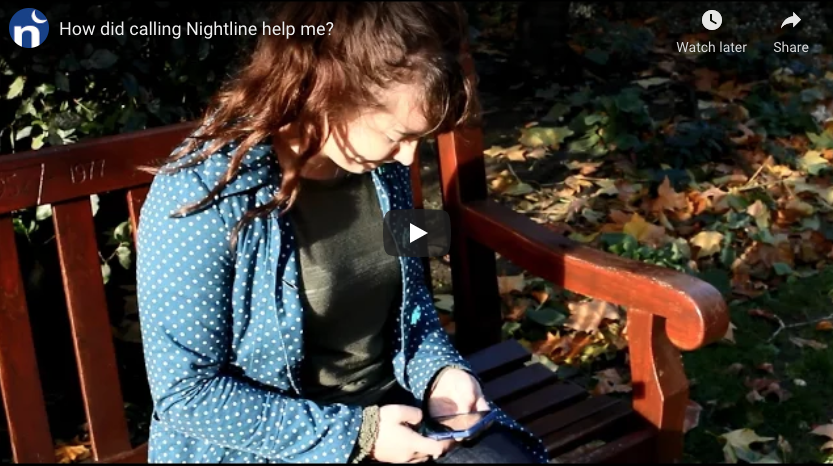
\includegraphics[width=0.99\linewidth]{images/youtube-nightline} 

}

\caption{Students explain in their own words how calling Nightline helped them whilst at university. [@youtube-nightline]}\label{fig:nightline-fig}
\end{figure}

Manchester students can contact nightline at \href{mailto:nightmail@nightline.manchester.ac.uk}{\nolinkurl{nightmail@nightline.manchester.ac.uk}} and expect a reply within 48 hours. See \href{https://manchester.nightline.ac.uk/}{manchester.nightline.ac.uk} for details.

\hypertarget{the-samaritans}{%
\subsection{The Samaritans}\label{the-samaritans}}

The \href{https://en.wikipedia.org/wiki/Samaritans_(charity)}{Samaritans} are a charity who provide emotional support to anyone in the the United Kingdom and Ireland that:

\begin{itemize}
\tightlist
\item
  is suffering from emotional distress
\item
  is struggling to cope
\item
  is at risk of suicide
\end{itemize}

The name of the charity comes from the \href{https://en.wikipedia.org/wiki/Parable_of_the_Good_Samaritan}{Parable of the Good Samaritan} although the organisation itself is not religious. The Samaritans are available 24 hours a day, seven days a week, to talk confidentially about any problem, however big or small. See \href{https://www.samaritans.org/}{samaritans.org} or telephone 116 123.

\hypertarget{students-against-depression}{%
\subsection{Students Against Depression}\label{students-against-depression}}

Students Against Depression (SAD) acknowledge the devastating impact that depression can have on those experiencing it, as well as on their friends, family and supporters. For further help in understanding and coping with suicidal thoughts, and emergency contacts in a crisis, visit \href{https://www.studentsagainstdepression.org/}{studentsagainstdepression.org}

Actor \href{https://en.wikipedia.org/wiki/Ruby_Wax}{Ruby Wax} has written about mental health and how the ``internal critics'' in our minds can send us mad in her book \emph{Sane New World}. \citep{sanenewworld} She is interviewed by Students Against Depression in the video in figure \ref{fig:rubywax-fig} about using mindfulness to ``dodge the bullets'' of depression.

\begin{figure}

{\centering 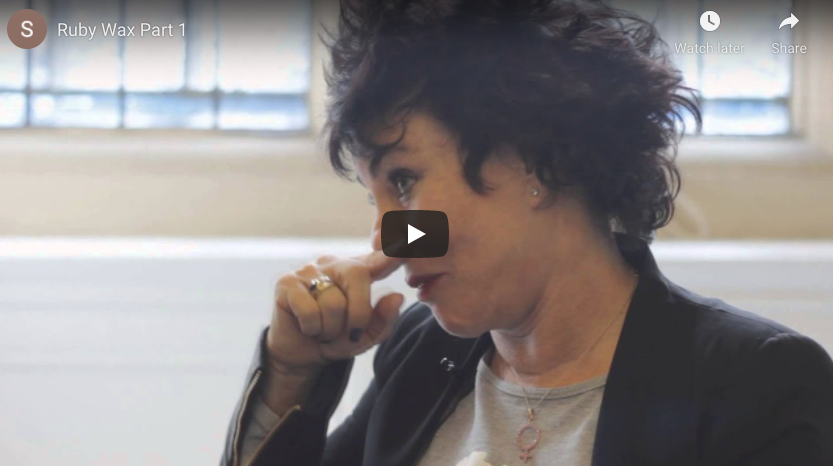
\includegraphics[width=0.99\linewidth]{images/youtube-wax} 

}

\caption{Ruby Wax describes being affected by depression in her childhood and how mindfulness and cognitive behavioural therapy (CBT) provided an alternative to medical treatment enabling her to dodge the bullets of mental health. [@youtube-wax]}\label{fig:rubywax-fig}
\end{figure}

\hypertarget{papryus}{%
\subsection{Papryus}\label{papryus}}

Suicide is the biggest killer of under 35's in the UK. Papyrus believe that many young suicides can be prevented, they are a national charity that you can find out more about at \href{https://www.papyrus-uk.org/}{papyrus-uk.org} or telephone the free number 0800 068 4141.

\hypertarget{self-help-services}{%
\subsection{Self-help services}\label{self-help-services}}

Self-Help services are a mental health charity which helps people to help themselves, see \href{https://www.selfhelpservices.org.uk/}{selfhelpservices.org.uk} or phone 0161 226 3871.

\hypertarget{mind}{%
\subsection{MIND}\label{mind}}

MIND provide advice and support to empower anyone experiencing a mental health problem. They campaign to improve services, raise awareness and promote understanding of mental health issues. Find out more at \href{https://www.mind.org.uk}{mind.org.uk} and in the video in figure \ref{fig:stephenfry-fig}

\begin{figure}

{\centering 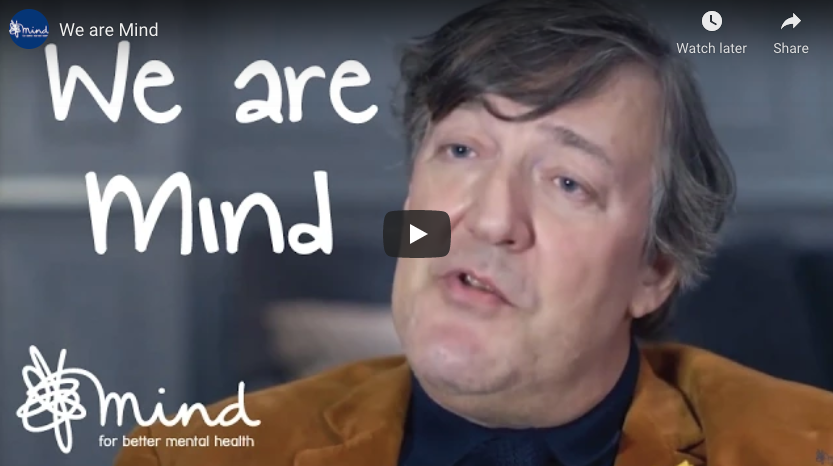
\includegraphics[width=0.99\linewidth]{images/youtube-we-are-mind} 

}

\caption{Stephen Fry, President of Mind, describes how MIND tackles misconceptions around mental health and social stigmas. [@youtube-we-are-mind] }\label{fig:stephenfry-fig}
\end{figure}

\hypertarget{student-minds}{%
\subsection{Student minds}\label{student-minds}}

Student Minds empowers students to look after their own mental health, support others and create change, find out more at \href{https://www.studentminds.org.uk}{studentminds.org.uk} and in the video in Figure \ref{fig:studentminds-fig} which describes why its important to talk about student mental health.

\begin{figure}

{\centering 
\includegraphics[width=0.99\linewidth]{images/youtube-student-minds} 

}

\caption{Talking about mental health is a crucial part of helping those who are suffering from it [@youtube-student-minds]}\label{fig:studentminds-fig}
\end{figure}

\hypertarget{togetherall}{%
\subsection{Togetherall}\label{togetherall}}

Togetherall is an online community for people who are stressed, anxious or feeling low. The service has an active forum with round-the-clock support from trained professionals. You can talk anonymously to other members and take part in group or 1-to-1 therapy with therapists. Togetherall is for anyone aged 16 or over who wants to improve their mental health. The service is free for many universities. Find out more at \href{https://togetherall.com/}{togetherall.com} and in the video in figure \ref{fig:togetherall-fig} which describes why its important to talk about student mental health.

\begin{figure}

{\centering 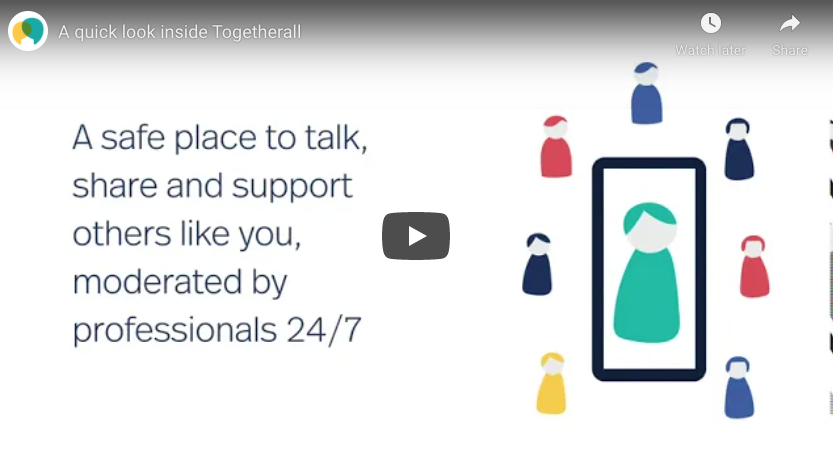
\includegraphics[width=0.99\linewidth]{images/youtube-togetherall} 

}

\caption{A quick look inside togetherall, an online community for people who are stressed, anxious or feeling low. [@youtube-togetherall]}\label{fig:togetherall-fig}
\end{figure}

\hypertarget{growthmindset}{%
\section{Developing a growth mindset}\label{growthmindset}}

Learning at University can be hard because you might have gone from being at (or near) the top of the class in high school to no longer being top of the class at University.

Likewise the \protect\hyperlink{searching}{job hunting we describe in the chapter on searching} can take a heavy toll on your mental health because repeated rejection is an ordinary part of the process. It can be time consuming, stressful and demoralising. You may find your applications disappear into a black hole. They will be ghosted (ignored) by employers. Interviewers will blank you and refuse to give you meaningful feedback because they're too busy. This could happen multiple times. This is all \emph{par for the course}, normal and expected, and is not necessarily a reflection on your abilities or potential.

\begin{figure}

{\centering \includegraphics[width=0.9\linewidth]{images/the-fixed-mindset} 

}

\caption{A fixed mindset is monolithic like the Easter island statues, known as \href{https://en.wikipedia.org/wiki/Moai}{Moʻai}. If you're not already, you should be wary of a fixed mindset. \href{https://bryanmmathers.com/fixed-mindsets/}{Fixed mindsets} by \href{https://visualthinkery.com}{Visual Thinkery} is licensed under \href{https://creativecommons.org/licenses/by-nd/4.0/}{CC-BY-ND}}\label{fig:fixedminset-fig}
\end{figure}



Adopting a growth mindset can be a successful strategy for maintaining your wellbeing, see figure \ref{fig:fixedminset-fig}. If your grades aren't has good as you hoped or your search for employment is being met with repeated rejection, a growth mindset can help. Let's take rejection from potential employers as an example, there are two ways you can react to it:

\begin{enumerate}
\def\labelenumi{\arabic{enumi}.}
\tightlist
\item
  \textbf{\emph{Fixed mindset}}: responding with a fixed mindset will mean you are likely to take rejection personally. You might even assume that this confirms what you've always suspected. You're not good enough or that you made some fatal mistake in your applications or interviews. Ouch.
\item
  \textbf{\emph{Growth mindset}}: by responding to rejection with a growth mindset, you focus on what happens next. Rejection is not failure but a ``not yet'' described in figure \ref{fig:not-fig}. Maybe you're not yet ready for that employer, but you'll definitely have a good idea of what you learned from the process and how can you do better next time.
\end{enumerate}

According to Stanford psychologist \href{https://en.wikipedia.org/wiki/Carol_Dweck}{Carol Dweck} we can all be placed on a spectrum according to where we think our abilities come from. At one end, the fixed mindset assumes all kinds of abilities are fixed traits while at the other end, a growth mindset assumes these abilities can be developed over time. \citep{dweck} There is good evidence to suggest that adopting a growth mindset will make you a better learner who can cope with the inevitable failures and rejections in life better. This approach can be used in a range of different disciplines such as learning programming languages \citep{Cutts2010}, music \citep{Davis2016} and job hunting.

\begin{figure}

{\centering 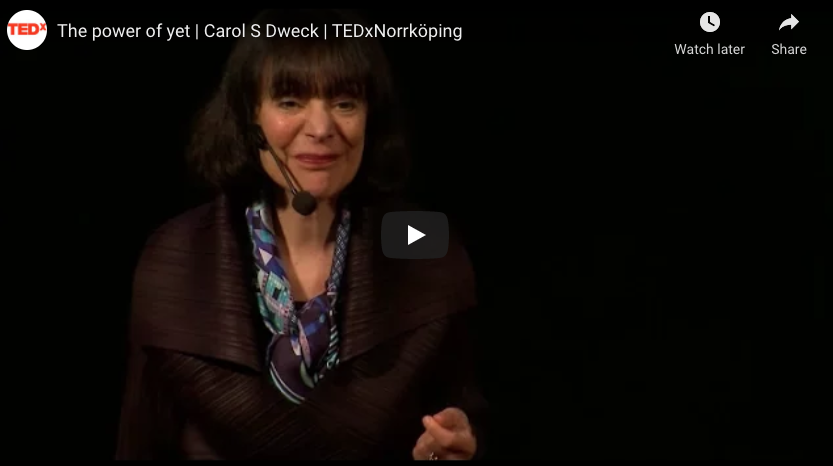
\includegraphics[width=0.99\linewidth]{images/youtube-dweck} 

}

\caption{Psychologist Carol Dweck explains the power of ``not yet'' and the growth mindset \citep{youtube-dweck}}\label{fig:not-fig}
\end{figure}



\hypertarget{signposts3}{%
\section{Wellbeing signposts}\label{signposts3}}

This chapter has looked at your wellbeing and especially the role that both your mental health and physical health play in your future. \href{https://en.wikipedia.org/wiki/Matt_Haig}{Matt Haig}'s first-hand accounts of poor mental health will be comforting to anyone who is affected by mental ill health. Even if you're not affected, there is a 25\% chance you will do at some point in your life. There's also a high probability someone close to you will suffer from mental health issues. It might be a colleague, friend, family member, fellow student or partner, so it is worth educating yourself on the issues by reading his two short books:

\begin{enumerate}
\def\labelenumi{\arabic{enumi}.}
\tightlist
\item
  \emph{Notes on a Nervous Planet} is a personal account of anxiety \citep{nervousplanet}
\item
  \emph{\href{https://en.wikipedia.org/wiki/Reasons_to_Stay_Alive}{Reasons to Stay Alive}} is a personal account of depression \citep{stayalive}
\end{enumerate}

What's good about Matt Haig's books is they are quick and easy to read, but give plenty of first-hand insight into what mental ill-health can do to people (including you). Matt describes his top five tips for good mental health in figure \ref{fig:haig-fig}

\begin{figure}

{\centering 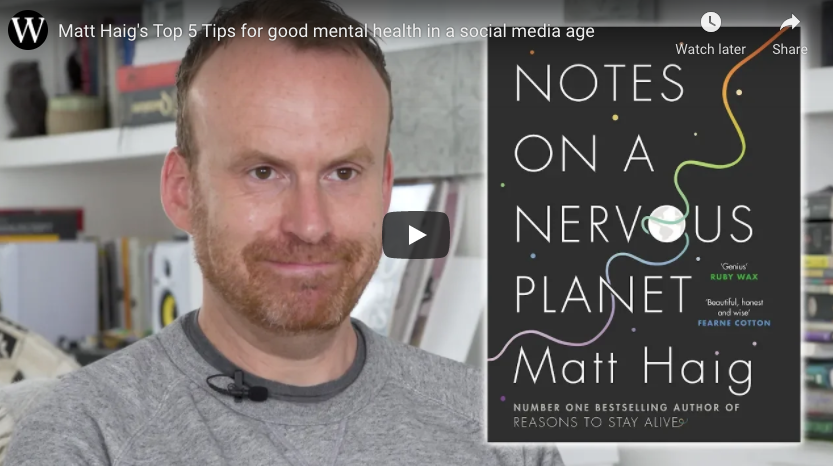
\includegraphics[width=0.99\linewidth]{images/youtube-haig} 

}

\caption{Two of Matt Haig's top five tips for good mental health \citep{youtube-haig} include 1. Being more careful (and mindful) of social media and 2. Reading more books because books are good for your soul. Not just his book. Any book. Books are good for you. Trust me on this. \citep{bookfriends}}\label{fig:haig-fig}
\end{figure}



There's plenty of evidence to suggest that social media can have a detrimental effect on health. \href{https://en.wikipedia.org/wiki/Jaron_Lanier}{Jaron Lanier}'s skeptical polemic \emph{Ten Arguments for Deleting Your Social Media Accounts Right Now} \citep{lanier} is a thought-provoking romp through some of the pitfalls of social media that may have you reaching for the delete or un-install button fairly quickly. You don't have to be on social media, see figure \ref{fig:socialmedia-fig}.

\begin{figure}
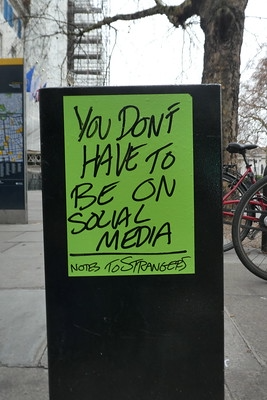
\includegraphics[width=0.32\linewidth]{images/you-dont-have-to-be-on-social-media} 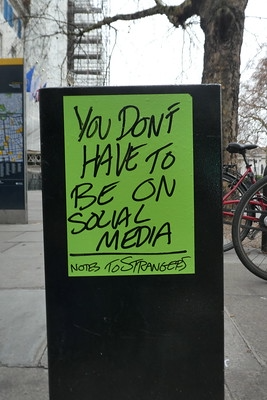
\includegraphics[width=0.32\linewidth]{images/you-dont-have-to-be-on-social-media} 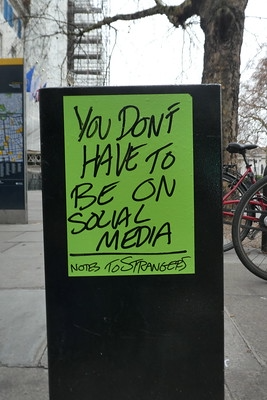
\includegraphics[width=0.32\linewidth]{images/you-dont-have-to-be-on-social-media} \caption{Social media like LinkedIn clearly has its uses (see \href{https://www.cdyf.me/debugging.html?q=linkedin\#links}{debugging your links}) but you you don't \emph{have} to be on it at all. Poor mental health is just one reason to be wary of social media, for nine other reasons read Jaron Lanier's polemic. \citep{lanier} You don't have to be on social media by \href{http://www.andy-leek.com/}{andy-leek.com} photographed by \href{https://www.flickr.com/photos/duncan/51014540593}{Duncan Cumming}}\label{fig:socialmedia-fig}
\end{figure}



If all these books are making you sleepy, neuroscientist Matthew Walker's \emph{\href{https://en.wikipedia.org/wiki/Why_We_Sleep}{Why We Sleep: The New Science of Sleep and Dreams}} may change your view on the importance of a good nights sleep. \citep{whywesleep}

Finally, it's well worth taking a look at \href{https://en.wikipedia.org/wiki/Laurie_R._Santos}{Laurie Santos} course on \emph{The Science of Wellbeing} (TSOWB) at \href{https://www.coursera.org/learn/the-science-of-well-being}{coursera.org/learn/the-science-of-well-being}. \citep{lauriesantos} TSOWB course provides an alternative to medication as it follows the principles of cognitive behavioural therapy (CBT).

TSOWB is the most popular course at Yale University and looks at some simple techniques you can use to improve your happiness. \citep{happinessny} The course will help you increase your happiness and build more productive habits. Using the latest research, Santos describes the misconceptions about happiness and ``annoying features'' of your mind that can impair your well-being. The course takes about 19 hours to complete but you can spread this over a whole semester (or longer) if you choose. The short clip in figure \ref{fig:laurie-fig} gives you a brief taster of Laurie's style and work.

\hypertarget{tldr3}{%
\section{Summarising well-being}\label{tldr3}}

\href{https://en.wiktionary.org/wiki/too_long;_didn\%27t_read}{Too long, didn't read} (TL;DR)? Here's a summary:

Anxiety and depression are serious conditions that are very likely to affect you or somebody close to you while you are at University. There's a one in four chance that you will be affected by mental health issues at some point in your life.

We've only talked about two particular mental health issues, anxiety and depression, but there are many other conditions such as phobias, obsessive-compulsive disorder (OCD), eating disorders, self-harm and more that are beyond the scope of this chapter. They do have one thing in common, and that is that talking about them is an important part of starting to develop better mental health.

If you are affected by mental ill health, talking about it is the first place to start, but often the hardest. In this chapter, I've outlined some ways you can help yourself alongside some of the services and people you can talk to if you need to.

Despite how you might feel, you are not alone.

Take my thoughts with you and when you look behind, you will surely see, a face that you recognise, you're not alone. \citep{yourenotalone}

\hypertarget{communicating}{%
\chapter{Writing your future}\label{communicating}}

Let's get straight to the point of this chapter: your soft skills will take a \textbf{life time} to develop and are \textbf{really hard} use. Why? Because soft skills are about \emph{communicating} with and \emph{understanding} other people so that you can work \emph{together} as a team toward a shared goal. Your soft skills are hard. There are very few jobs where you work on your own, and most software and hardware is designed, built, tested and used by teams of people. Many of these teams are large and have very diverse membership. This means that sooner or later you're going to have to master the dark arts of \emph{working with other people} by deploying your softer skills. 😱

\begin{figure}

{\centering \includegraphics[width=1\linewidth]{images/What - other people} 

}

\caption{Unless you want to be a \href{https://en.wikipedia.org/wiki/Lighthouse_keeper}{lighthouse keeper} on a remote island, there are very few jobs where you don't have to work as part of a team with other people. Sorry to break the bad news! This means you need to constantly improve your softer skills and provide evidence of them to potential employers. Other people sketch by \href{https://visualthinkery.com}{Visual Thinkery} is licensed under \href{https://creativecommons.org/licenses/by-nd/4.0/}{CC-BY-ND}}\label{fig:otherpeople-fig}
\end{figure}



Communicating with other people and working in teams is inherently difficult because we're all human. There is good news and bad news\ldots{}

\begin{itemize}
\tightlist
\item
  \textbf{THE GOOD NEWS} is, people can be diligent, humble, competent, honest, caring and reliable. They can be co-operative, generous, supportive, kind, thoughtful, intelligent, sensitive, understanding, punctual and professional too!
\item
  \textbf{THE BAD NEWS} is, unfortunately people can also be lazy, stupid, ignorant, vain, incompetent, dishonest, unreliable, greedy, egomaniacal, unpredictable and moody. They can be proud, selfish, competitive, lustful, angry, envious, mean, busy, insensitive and thoughtless too. Some will disagree with you, boss you around, betray, exploit, misunderstand and mislead you, deliberately or otherwise. \citep{sevendeadly}
\end{itemize}

So communicating with and understanding other people can be hard work, but don't worry, \textbf{everyone} finds this challenging, it's not just you! It doesn't matter if you're an extrovert or an introvert, we \emph{all} find communication difficult, and everyone can get better at it. This chapter takes a look at the softer skills and techniques you can use to improve your communication with other people, whatever mood they are in and whosever team they are on.

\hypertarget{what-you-will-learn}{%
\section{What you will learn}\label{what-you-will-learn}}

\begin{itemize}
\tightlist
\item
  Recognise the importance of written communication, both as a reader and a writer
\item
  Identify examples of where written communication is crucial in science and engineering
\item
  Improve your written communication skills using some simple writing and reading exercises
\item
  Identify the importance of teamwork
\end{itemize}

\hypertarget{computing-is-your-superpower}{%
\section{Computing is your superpower!}\label{computing-is-your-superpower}}

Studying computer science gives you an awesome superpower. We will look at some of the reasons why in the chapter on \protect\hyperlink{computing}{Computing your Future}. But for now, let us just acknowledge that hard technical skills like computing are highly sought after and valuable, both commercially and otherwise.

\begin{figure}

{\centering \includegraphics[width=1\linewidth]{images/Achilles-Heel-to-Superpower} 

}

\caption{Computing is a superpower that gods like \href{https://en.wikipedia.org/wiki/Hermes}{Hermes} and mortal heroes like \href{https://en.wikipedia.org/wiki/Achilles}{Achilles} would probably have envied. \citep{heroes} As a technical or ``hard skill'', computing is a crucial weapon in your armoury but what are your weaker skills? What is your \href{https://en.wikipedia.org/wiki/Achilles\%27_heel}{Achilles' heel}? For some scientists and engineers, their weakness is their soft skills, such as communication and team work. This chapter looks at what you can do to improve them and convince employers that you are rounded individual with a healthy balance of soft and hard skills. \href{https://bryanmmathers.com/achilles-heel-to-superpower/}{Achilles heel to superpower} by \href{https://visualthinkery.com/s}{Visual Thinkery} is licensed under \href{https://creativecommons.org/licenses/by-nd/4.0/}{CC-BY-ND}}\label{fig:achilles-fig}
\end{figure}



Your computational superpower is less powerful if it isn't complemented by a broad range of softer skills. Typically, these skills are not emphasised (by repeated assessment) in most computer science degrees. This not because soft skills aren't important but because they are hard to measure accurately.

For example, if I want to know how good you are at understanding the syntax and semantics of a programming language like Python, there are tried and tested techniques for doing this. However, if I want to know how good you are at using your communication skills to work in a team, negotiate, lead, resolve conflicts, persuade others, show empathy etc that's \textbf{much} harder to measure accurately.

\begin{figure}

{\centering \includegraphics[width=1\linewidth]{images/Hard and soft skills} 

}

\caption{Hard skills and soft skills aren't much use without each other. You will need both to survive and thrive but most science and engineering education focuses on your hard skills, not your soft skills. Why? Because hard skills are often much easier to measure. Hard and soft skills sketch by \href{https://visualthinkery.com/}{Visual Thinkery} is licensed under \href{https://creativecommons.org/licenses/by-nd/4.0/}{CC-BY-ND}}\label{fig:allskills-fig}
\end{figure}



Let's look at some of low-level communication skills (I/O) that they are built on.

\hypertarget{communication-i0}{%
\section{Communication I/0}\label{communication-i0}}

In terms of input and output, your fundamental communication skills are listening, speaking, reading and writing words in natural languages shown in table \ref{tab:iotable}. These are the ``\href{https://en.wikipedia.org/wiki/Assembly_language}{assembly languages}'' of human communication. This might sound blindingly obvious, but these skills are often under-estimated or undervalued by engineers and scientists, especially undergraduates. Alongside verbal and written communication, there's also nonverbal language, or body language such as eye contact, gestures and facial expressions.

\begin{table}

\caption{\label{tab:iotable}The inputs and outputs of the fundamental assembly languages of human communication }
\centering
\begin{tabular}[t]{lll}
\toprule
 & Input & Output\\
\midrule
Written natural language & Reading & Writing\\
Spoken natural language & Listening & Speaking\\
Nonverbal language & Observing other people & Being observed by others\\
\bottomrule
\end{tabular}
\end{table}

Engineers and scientists sometimes lack communication skills outlined in table \ref{tab:iotable}. Think of your stereotypical scientist, clad in a white coat, unable to explain the complexities of their subject to people inside their lab, let alone outside of it. Then there is the nerdy software engineer stereotype who prefers the company of computers to people. Yes, these are lazy and sometimes unhelpful stereotypes, but they express public perception of scientists and engineers as poor communicators.

\hypertarget{mightier}{%
\subsection{The pen is mightier than the sword}\label{mightier}}

The art of communication is a huge subject which extends far beyond the scope of this guidebook. So for the rest of this chapter, we'll focus on written communication skills because:

\begin{enumerate}
\def\labelenumi{\arabic{enumi}.}
\tightlist
\item
  \textbf{Good writing and reading are crucial in applications} for employment and further study. From writing CV's, covering letters, completing application forms and reading job specifications, and employer or course information, your ability to read and write natural languages is crucial to coding your future.
\item
  \textbf{Writing often gets neglected}: Written communication skills (both reading and writing) are sometimes sidelined in science and engineering degrees. This is particularly true in the ``hard sciences''. For example, communicating and solving problems using code or mathematics are usually the dominant forms of assessment in computer science courses. That's understandable given the subject, but tends to push natural languages like english to the sidelines.
\item
  \textbf{Good engineers are also good writers} Many engineers (and scientists) could significantly improve their written communication skills. Software engineers are notoriously bad at writing good documentation, see for example \href{https://dl.acm.org/doi/10.1145/960492.960525}{Why Computer Science Students Need Language}, \citep{Beaubouef2003} \emph{Scientists Must Write} \citep{scientistsmustwrite} and \href{https://www.theatlantic.com/national/archive/2012/10/the-real-reason-silicon-valley-coders-write-bad-software/263377/}{The Real Reason Silicon Valley Coders Write Bad Software}, \citep{writebadsoftware} just three examples amongst many others making exactly the same point. Employers like Google provide training (and a whole career path) for technical writers, see \href{https://developers.google.com/tech-writing}{developers.google.com/tech-writing}. However, I'm arguing that these careers wouldn't be needed if software engineers were better at documenting, explaining and communicating with other human beings their code in the first place!
\item
  \textbf{Writing good english is like writing good code}. Some of the skills you already have in coding can be transferred to written communication. Just like a good function or method in code should be well-defined with a clear purpose, your writing should also be clear and coherent. Well structured writing is a lot like well architected software too, with a clear \href{https://en.wikipedia.org/wiki/Separation_of_concerns}{separation of concerns} (SoC)
\item
  \textbf{It is relatively easy to improve} your written communication skills, simply by reading and writing more. Reading and writing deliberately every day, will significantly improve these skills.
\end{enumerate}

\hypertarget{nle}{%
\subsection{Natural language engineering}\label{nle}}

If you stop to think about it, engineers and scientists spend a \emph{lot} time communicating in writing. As well as engineering code, they also spend a significant amount of time engineering messages in natural languages like english. Consider the following:

\begin{itemize}
\tightlist
\item
  email and instant messaging, Slack, Microsoft Teams, Discord, Zoom etc
\item
  Posting on social media: LinkenIn, Facebook, WhatsApp, Twitter, blogs, Medium.com etc
\item
  bug reports and messages in \href{https://en.wikipedia.org/wiki/Comparison_of_issue-tracking_systems}{issue trackers} like Jira, BugZilla and Trello
\item
  `How to' and cookbook style articles and books
\item
  API reference material
\item
  in-code documentation \texttt{\#\ comments\ in\ code}
\item
  \href{https://en.wikipedia.org/wiki/Self-documenting_code}{Self-documenting code}
\item
  Executable specifications in test suites like \href{https://en.wikipedia.org/wiki/Cucumber_(software)}{cucumber.io}
\item
  Laboratory manuals and laboratory notebooks
\item
  The one page summary for management
\item
  User documentation, release notes
\item
  Case studies of software use
\item
  Frequently Asked Questions (FAQ)
\item
  YourPersonalDomain.com (if you have one)
\item
  Questions and answers on forums like \href{https://stackoverflow.com/}{stackoverflow.com}
\item
  Commit messages in version control systems like git and mercurial etc
\item
  Architecture documentation and design specifications
\item
  \href{https://en.wikipedia.org/wiki/Literate_programming}{Literate programming} natural language descriptions of computational logic \citep{knuthlit}
\item
  \href{https://jupyter.org/}{Jupyter.org notebooks}, code and natural language mixed together
\item
  \href{https://bookdown.org/}{bookdown.org} mixes code and natural language
\end{itemize}

What do they all have in common? They're all written in natural languages like the \href{English\%20language}{English language}, but without them, the software or hardware they describe and discuss would be useless.

\hypertarget{writing-your-future}{%
\section{Writing your future}\label{writing-your-future}}

Hopefully I've convinced you that written communication skills (both as a writer and reader) are important soft skills that engineers often neglect. So how can you improve?

\hypertarget{try-googles-tech-writing-course}{%
\subsection{Try Google's Tech Writing course}\label{try-googles-tech-writing-course}}

Google have developed some excellent technical writing courses including:

\begin{enumerate}
\def\labelenumi{\arabic{enumi}.}
\tightlist
\item
  Technical Writing One: Technical Writing Fundamentals for Engineers \href{https://developers.google.com/tech-writing/one}{developers.google.com/tech-writing/one}
\item
  Technical Writing Two: Intermediate Technical Writing for Engineers \href{https://developers.google.com/tech-writing/two}{developers.google.com/tech-writing/two}
\end{enumerate}

These courses run as part of the second year course COMP2CARS at the University of Manchester, see \protect\hyperlink{scheduling}{the course schedule for details}

Google occasionally delivers these technical writing courses as free sessions open to the general public. For details, see \href{https://developers.google.com/tech-writing/announcements}{developers.google.com/tech-writing/announcements} for details.

\hypertarget{deliberate-daily-writing}{%
\subsection{Deliberate daily writing}\label{deliberate-daily-writing}}

Another technique for improving your written communication is to write something every day, that might be a personal diary that only you read, or it could be something more public like blog. Schedule a time every day, say 15 to 30 minutes when you will do this without fail. That writing could take several forms:

\begin{itemize}
\tightlist
\item
  private diary
\item
  \href{https://en.wikipedia.org/wiki/Gratitude_journal}{gratitude journal}
\item
  public web log or \href{https://en.wikipedia.org/wiki/Blog}{blog}
\item
  personal notes gathered somewhere (e.g.~private github repository)
\item
  \href{https://en.wikipedia.org/wiki/Bullet_journal}{bullet journal}. Some people swear by it, see \href{https://bulletjournal.com/}{bulletjournal.com}
\end{itemize}

The technique of \emph{30 minutes per day} can be a very effective way of getting things done, incrementally over time. In my experience it works for lots of things besides writing including getting exercise (discussed in the \href{wellbeing.html}{wellbeing chapter}) to gardening. \citep{leendertz}

\hypertarget{deliberate-daily-reading}{%
\subsection{Deliberate daily reading}\label{deliberate-daily-reading}}

Reading other people's code will improve your software engineering skills. Likewise, reading other peoples writing will improve your natural language engineering skills. Read anything, it might be novels, magazines, newspapers, stuff online or any of the books cited in the \href{references.html}{references}. Find a time and place to do this every day and stick to it.

\hypertarget{dogfooding}{%
\subsection{Dogfooding}\label{dogfooding}}

Some companies test their products by trialling them on their own employees, this is sometimes known as \href{https://en.wikipedia.org/wiki/Eating_your_own_dog_food}{eating your own dogfood}. Tasty, tasty dogfood. 🐶

You can use a similar approach to testing your own writing, known simply as \textbf{Dogfooding}. Let's say you've just written a covering letter. It's natural to read it over in your head to check for errors, before you send it. However, \textbf{reading it aloud} will pick up errors you may not have spotted by reading silently. There's something about articulating words out loud that flushes out errors you don't pick up when you read them. This is a tried and tested technique. It also means you're ready to vocalise those answers in an interview.

You might want to choose carefully where you do this as it might look a bit strange, but it works well. If you talk into a mobile phone while looking at a piece of paper, people won't notice you're talking to yourself. But you'll probably need some privacy as the stuff you're talking about is likely to be personal.

\hypertarget{rtfm}{%
\subsection{Reading the friendly manual}\label{rtfm}}

You don't get good at communicating with computers (coding) by just \emph{writing} lots of code. You also need to \emph{read} other people's code too and be able to understand and modify it. Likewise, you don't get good at communicating with people by just \emph{writing} stuff in natural languages like english. You need to \emph{read} stuff too. Books, manuals, software documentation, articles, use cases, novels, poetry, plays, magazines, newspapers etc. Reading this stuff will help you learn and you'll improve your written communication skills too. So Read The Friendly Manual. \href{https://en.wikipedia.org/wiki/RTFM}{RTFM}. Read THIS Friendly Manual, see figure \ref{fig:rtfm-fig}

\begin{figure}

{\centering \includegraphics[width=0.9\linewidth]{images/RTFM} 

}

\caption{As well as learning from other people's hard won experience, reading the friendly manual (\href{https://en.wikipedia.org/wiki/RTFM}{RTFM}) will also improve you written communication skills. Just like you improve your coding skills by writing and reading code, improve your written communication skills by reading and writing in natural langauges like English. RTFM poster by Jeremy Keith, modified by \href{https://commons.wikimedia.org/wiki/User:Atlasowa}{Atlaslowa} is licensed under \href{https://creativecommons.org/licenses/by/2.0/deed.en}{CC-BY} on Wikimedia Commons \href{https://w.wiki/vBX}{w.wiki/vBX}}\label{fig:rtfm-fig}
\end{figure}



\hypertarget{coding-challenges}{%
\section{Coding challenges}\label{coding-challenges}}

\begin{itemize}
\tightlist
\item
  Write an article or blog post about something you care about, find a suitable venue for publication
\item
  Take a course from outside computer science, where the main form of assessment is written essays or dissertations. Humanities departments are a good place to start. This will improve your written communication skills
\item
  Not been reading many books lately? Pick a book to read just because its interesting, rather than because you have to.
\end{itemize}

\hypertarget{tldr4}{%
\section{Summarising your soft skills}\label{tldr4}}

\href{https://en.wiktionary.org/wiki/too_long;_didn\%27t_read}{Too long, didn't read} (TL;DR)? Here's a summary:

You'll need both soft and hard skills to compete in the workplace. Don't underestimate the importance of softer skills, we've looked briefly at written communication skills in this chapter but that's only the tip of the soft skills iceberg.

Teamwork, negotiation, conflict resolution, motivation and leadership are other soft skills that are important too. How can you develop these skills while at University? How can you demonstrate to potential employers that you have these skills?

This chapter is under construction because I'm using agile space station development methods, see figure \ref{fig:deathstar-fig}.

\begin{figure}

{\centering \includegraphics[width=0.32\linewidth]{images/DeathStar2} 

}

\caption{This chapter is under construction. Image of the \href{https://en.wikipedia.org/wiki/Death_Star}{Death Star} via Wikimedia Commons \href{https://w.wiki/32PB}{w.wiki/32PB}}\label{fig:deathstar-fig}
\end{figure}



\hypertarget{experiencing}{%
\chapter{Experiencing your future}\label{experiencing}}

So, tell me, are you experienced? Why is experience valuable and what kind of experience are employers looking for anyway? How can you get some more experience? 🤔

\begin{figure}

{\centering \includegraphics[width=1\linewidth]{images/404} 

}

\caption{Do you respond with a sheepish \emph{experience not found} error message when people ask about your experience? Is your experience like the \href{https://en.wikipedia.org/wiki/HTTP_404}{classic HTTP 404} page not found? The client sent you a valid request for your experience, but your server couldn't find it. Awkward. Embarrassing silence? 😳 Don't worry, there are some simple and easy ways to build your experience so that instead of negative 404's, you can respond with a cheerfully positive 200 (OK), as described in this \href{https://en.wikipedia.org/wiki/List_of_HTTP_status_codes}{list of HTTP status codes}. We'll look at some of them in this chapter. Experience not found sketch by \href{https://visualthinkery.com/}{Visual Thinkery} is licensed under \href{https://creativecommons.org/licenses/by-nd/4.0/}{CC-BY-ND}}\label{fig:404-fig}
\end{figure}



\hypertarget{ilo5}{%
\section{What you will learn}\label{ilo5}}

By the end of this chapter you will be able to

\begin{itemize}
\tightlist
\item
  Describe why having experience can improve your chances of getting interviews
\item
  Identify what counts as experience and why it's valuable
\item
  Recognise opportunities to get more experience before you graduate
\end{itemize}

\begin{figure}

{\centering \includegraphics[width=1\linewidth]{images/What's relevant} 

}

\caption{You might be surprised by which of your experiences are relevant, and what kinds of experience are relevant on your CV. What's relevant sketch by \href{https://visualthinkery.com/}{Visual Thinkery} is licensed under \href{https://creativecommons.org/licenses/by-nd/4.0/}{CC-BY-ND}}\label{fig:relevance-fig}
\end{figure}



\hypertarget{why-is-experience-so-valuable}{%
\section{Why is experience so valuable?}\label{why-is-experience-so-valuable}}

It's common for students to be focused on their grades, whether those grades are low, middling or or high. At the extremes, if you have got lower grades than you'd like, you might be anxious or unhappy about them. If you've got higher grades, you're probably focussed on keeping them high. Either way, you are \emph{much more} than your grades, because your education is only a part of who you are, shown in in figure \ref{fig:not-just-grades-fig}. You are the sum total of your experiences, this is one of the reasons that experience is so valuable.

\begin{figure}

{\centering \includegraphics[width=1\linewidth]{images/i-am-more-than-just-my-grades} 

}

\caption{There is a lot more to you than your grades. Your experience tells people much more about your character, not just paid work, but any voluntary work and projects you've been involved in too. \href{https://bryanmmathers.com/i-am-more-than-just-my-grades/}{I am more than just my grades} sketch by \href{https://visualthinkery.com/}{Visual Thinkery} is licensed under \href{https://creativecommons.org/licenses/by-nd/4.0/}{CC-BY-ND}}\label{fig:not-just-grades-fig}
\end{figure}



\hypertarget{areuexperienced}{%
\section{Are you experienced?}\label{areuexperienced}}

So what counts as experience?

\begin{itemize}
\tightlist
\item
  Freelance work: being self-employed
\item
  Insight programmes and spring weeks: work shadowing
\item
  Part-time jobs: casual or part-time work
\end{itemize}

\hypertarget{bignames}{%
\subsection{Big name experience}\label{bignames}}

It's easier than you might think to get a big name on your CV. For example, many large employers run \href{https://www.ratemyplacement.co.uk/insights}{insight days, vacation schemes and spring weeks}. These are often aimed at first years, and are sometimes less competitive to get into than a longer term commitment such as a summer internship, year-long placement or even graduate job. A big name on your CV early in your degree can help it stand out later, as fluff bucket the grinning \href{https://en.wikipedia.org/wiki/Cheshire_Cat}{cheshire cat} demonstrates on their CV shown in \ref{fig:bigname-fig}. 😻

\begin{figure}

{\centering \includegraphics[width=1\linewidth]{images/Big Name} 

}

\caption{It's easier than you might think to get a big name on your CV, sometimes these can help your application stand out from the competition. Big name sketch by \href{https://visualthinkery.com}{Visual Thinkery} is licensed under \href{https://creativecommons.org/licenses/by-nd/4.0/}{CC-BY-ND}}\label{fig:bigname-fig}
\end{figure}



Other ways to get a big name on your CV include joining a big name competition or event, for example:

\begin{itemize}
\tightlist
\item
  IBM hosts the annual Call for Code \href{https://developer.ibm.com/callforcode}{developer.ibm.com/callforcode}
\item
  Google has

  \begin{itemize}
  \tightlist
  \item
    Code Jam, HashCode and Kick Start \href{https://codingcompetitions.withgoogle.com/}{codingcompetitions.withgoogle.com}
  \item
    Summer of Code \href{https://summerofcode.withgoogle.com/}{summerofcode.withgoogle.com}
  \end{itemize}
\item
  Facebook has hackathons, see \href{https://en-gb.facebook.com/hackathon}{facebook.com/hackathon} and \href{https://developers.facebook.com/}{developers.facebook.com}
\item
  Microsoft hosts the Imagine Cup \href{https://imaginecup.microsoft.com/}{imaginecup.microsoft.com}
\item
  There are many others like these listed at \href{https://devpost.com}{devpost.com}, Major League Hacking \href{https://mlh.io/}{mlh.io} and Hacker Earth \href{https://www.hackerearth.com/}{hackerearth.com} etc
\end{itemize}

Big names can look good on your CV, but they are not the only way to make your CV stand out.

\hypertarget{volunteering}{%
\subsection{Voluntary experience}\label{volunteering}}

Experience in the CV sense usually means paid work. However, experience in the context of \emph{are you experienced?} \citep{hendrix} means anything where you can show you've been part of a bigger team, taken responsibility for something or tried to make the world a better place somehow. These include:

\begin{itemize}
\tightlist
\item
  Volunteering: Doing voluntary work is a good way to pick up new skills
\item
  Being involved in societies: e.g.~taking responsibility for things in a society
\item
  Getting involved in a community, either physical or online
\item
  Fixing bugs in open source software
\end{itemize}

\hypertarget{casual}{%
\subsection{Casual experience}\label{casual}}

You may already have experience of paid employment as a casual or part-time worker. This could include jobs such as waiting tables, serving in a bar or working in other areas of hospitality or retail, for example as a Saturday job.

\begin{figure}

{\centering \includegraphics[width=0.5\linewidth]{images/Titanic-paperboy-crop} 

}

\caption{Casual and part-time work tell an important story about your on on your CV. For example, from the age of 11, I was a paperboy, delivering newspapers door to door to paying customers. This demonstrates reliability and work ethic, because I did this in all weathers (sun, wind, rain, snow, hangovers etc) for seven years, man and boy! If you have casual experience, don't forget to include it in your CV. Public domain image of the Titanic paperboy, Ned Parfett selling newspapers in London via Wikimedia Commons at \href{https://w.wiki/35HA}{w.wiki/35HA}}\label{fig:paperboy-fig}
\end{figure}



It is important to recognise that these jobs have value. Many students make the mistake of overlooking their casual work experience because they disregard it as non-technical or consider it ``low-skilled''. In the section on \protect\hyperlink{mycvst}{structuring your CV}, \citep{topnotchcv} one of the stories you want to tell in your job applications is that you:

\begin{enumerate}
\def\labelenumi{\arabic{enumi}.}
\tightlist
\item
  take responsibility
\item
  achieve things
\item
  are nice to have around
\end{enumerate}

Doing casual work can demonstrate all of these things. For example, from the ages of 11 to 18 I was a \href{https://en.wikipedia.org/wiki/Paperboy}{paperboy}, except unlike the one selling newspapers in the street in figure \ref{fig:paperboy-fig}, I delivered newspapers directly to the doors of paying customers every morning. This was not a particularly highly skilled job, but it \emph{does} demonstrate:

\begin{enumerate}
\def\labelenumi{\arabic{enumi}.}
\tightlist
\item
  \href{https://en.wikipedia.org/wiki/Work_ethic}{work ethic}: getting up early \emph{every} morning (including Saturdays). Sometimes work is about just turning up everyday!
\item
  taking responsibility and being reliable
\item
  understanding the value of money by earning a wage
\end{enumerate}

If you have experience of working in retail, such as serving customers in a supermarket, this also demonstrates your ability to provide good customer service and work as part of a team. This is the ``nice to have around'' bit that Jonathan Black refers to \citep{topnotchcv} and is something your formal education will not typically provide any evidence of. So don't fall into the trap of discounting the value of casual or part-time labour.

\hypertarget{tldr5}{%
\section{Summarising your experience}\label{tldr5}}

\href{https://en.wiktionary.org/wiki/too_long;_didn\%27t_read}{Too long, didn't read} (TL;DR)? Here's a summary:

This chapter is under construction because I'm using agile space station development methods, see figure \ref{fig:deathstar2-fig}.

\begin{figure}

{\centering \includegraphics[width=0.32\linewidth]{images/DeathStar2} 

}

\caption{This chapter is under construction. Image of the \href{https://en.wikipedia.org/wiki/Death_Star}{Death Star} via Wikimedia Commons \href{https://w.wiki/32PB}{w.wiki/32PB}}\label{fig:deathstar2-fig}
\end{figure}

\hypertarget{computing}{%
\chapter{Computing your future}\label{computing}}

It's difficult to think of any aspect of our lives that hasn't been changed by the invention of the digital computer, just 70 short years ago. Consequently, computing is a crucial skill in a wide range of careers across every sector of business and society. You don't have to have studied Computer Science at University to take advantage of all the exciting opportunities provided by computing. This chapter looks at some of those opportunities for those with, and without, degrees in Computer Science. 👨🏿‍💻👨‍💻👩🏽‍💻👩‍💻👨🏿‍💻

\begin{figure}

{\centering \includegraphics[width=1\linewidth]{images/not just about coding} 

}

\caption{Computing is much more than coding, this chapter looks at what computing can do for your future. CV work sketch by \href{https://visualthinkery.com}{Visual Thinkery} is licensed under \href{https://creativecommons.org/licenses/by-nd/4.0/}{CC-BY-ND}}\label{fig:not-coding-fig}
\end{figure}



\hypertarget{ilo6}{%
\section{What you will learn}\label{ilo6}}

Reading this chapter and doing the activities will help you to:

\begin{itemize}
\tightlist
\item
  Describe why computing is a stimulating and challenging subject to study in its own right
\item
  Identify roles where studying computer science is relevant, beyond software engineering
\item
  Describe why NOT studying computer science doesn't necessarily ``lock you out'' of doing taking on some of these roles
\end{itemize}

\hypertarget{copps}{%
\section{Computing: your future?}\label{copps}}

What role will computing play in your future career? A Professor of Computer Science at Princeton University, \href{https://en.wikipedia.org/wiki/Robert_Sedgewick_(computer_scientist)}{Robert Sedgwick}, has, like many others, argued that Computer Science should be required of all students:

\begin{quote}
Every college student needs a computer science course, and most need two or more. More and more educators are
beginning to recognize this truth, but we are a long way from meeting the need. --Robert Sedgwick \citep{robertsedgwick}
\end{quote}

\hypertarget{joker}{%
\section{Computational joker}\label{joker}}

If academic disciplines are \href{https://en.wikipedia.org/wiki/Playing_card_suit}{playing card suits}, then Computer Science is the \href{https://en.wikipedia.org/wiki/Joker_(playing_card)}{joker in the pack} shown in figure \ref{fig:joker-fig}. A versatile card, the computational joker can be played with (and without) any of the traditional four suits: diamonds, clubs, hearts and spades. That's because computing is a science \emph{and} an art. It allows us to study human society and culture, so it's part of the \href{https://en.wikipedia.org/wiki/Humanities}{humanities} too. Last but not least, computing is also an engineering discipline and a branch of mathematics too. What all this means is that the computational joker is a \href{https://en.wikipedia.org/wiki/Wild_card_(cards)}{wild card} that can be played \emph{whenever and wherever} you like, making it an incredibly \href{broadening.html}{powerful but dangerous card}, depending on the game you are playing. ♣♥♠♦🃏

\begin{figure}

{\centering \includegraphics[width=1\linewidth]{images/wikijoker} 

}

\caption{Computer Science: The joker in the pack. Public domain image of the Jolly Joker, a vintage Masenghini Italian playing card via Wikimedia Commons \href{https://w.wiki/35EW}{w.wiki/35EW} adapted from the \href{https://en.wikipedia.org/wiki/Joker_(playing_card)}{joker playing card} using the \href{https://apps.apple.com/gb/app/wikipedia/id324715238}{Wikipedia app}.}\label{fig:joker-fig}
\end{figure}



\hypertarget{indemand}{%
\section{Developers in demand}\label{indemand}}

Demand of software developers (jokers?) is high, on a par with teaching and nursing in terms of numbers. For example, in the UK, the most common jobs for graduates from 2017-18 are shown in Figure \ref{fig:nurses-fig}, based on data taken from an article on \href{https://wonkhe.com/blogs/what-might-the-graduate-labour-market-look-like-in-2021/}{the graduate labour market in 2021} \citep{wonkyball}

\begin{figure}

{\centering \includegraphics[width=1\linewidth]{cdyf_files/figure-latex/nurses-fig-1} 

}

\caption{The most common jobs for graduates in the UK in 2017-18, demand for software developers is high according to data taken from \citep{wonkyball}}\label{fig:nurses-fig}
\end{figure}



\hypertarget{tldr6}{%
\section{Summarising computing your future}\label{tldr6}}

\href{https://en.wiktionary.org/wiki/too_long;_didn\%27t_read}{Too long, didn't read} (TL;DR)? Here's a summary:

This chapter is under construction because I'm using agile space station development methods, see figure \ref{fig:deathstar3-fig}.

\begin{figure}

{\centering \includegraphics[width=0.32\linewidth]{images/DeathStar2} 

}

\caption{This chapter is under construction. Image of the \href{https://en.wikipedia.org/wiki/Death_Star}{Death Star} via Wikimedia Commons \href{https://w.wiki/32PB}{w.wiki/32PB}}\label{fig:deathstar3-fig}
\end{figure}

\hypertarget{part-building-your-future}{%
\part{BUILDING YOUR FUTURE}\label{part-building-your-future}}

\hypertarget{debugging}{%
\chapter{Debugging your future}\label{debugging}}

It's all very well \emph{designing} your future but now you need to actually \emph{build} and \emph{test} it. An obvious place to start is with your CV, because that's where most people get going. How can you create a bug-free CV, resume or completed application form? How can you support applications with a strong personal statement or covering letter? How can you debug your future? 🐛

\begin{figure}

{\centering \includegraphics[width=1\linewidth]{images/Features not bugs} 

}

\caption{Is that a bug or a feature in your CV? To stand a chance of being invited to interview, you'll need to identify and fix any bugs in your written applications. If you don't, your application risks being sucked into a black hole and will never be seen again. Features not bugs picture by [Visual Thinkery](https://visualthinkery.com) is licensed under [CC-BY-ND](https://creativecommons.org/licenses/by-nd/4.0/)}\label{fig:bugfeature-fig}
\end{figure}

\hypertarget{ilo7}{%
\section{What you will learn}\label{ilo7}}

By the end of this chapter you will be able to

\begin{itemize}
\tightlist
\item
  Structure and style the content of CV /resume appropriately
\item
  Describe the context, actions and results (CAR) of your relevant experience, projects and education
\item
  Identify and fix bugs in CV's by:

  \begin{itemize}
  \tightlist
  \item
    Constructively criticising other people's CVs
  \item
    Asking for, listening to, and acting on constructive criticism of your own CV
  \end{itemize}
\item
  Quantify and provide evidence for any claims you make you on your CV
\end{itemize}

\hypertarget{blackhole}{%
\section{Beware of the black hole}\label{blackhole}}

Before we get started, let's consider some advice from software engineer \href{https://en.wikipedia.org/wiki/Gayle_Laakmann_McDowell}{Gayle Laakmann McDowell} shown in figure \ref{fig:gayle-fig}. Gayle is an experienced software engineer who has worked at the biggest technology employers in the world, Apple, Microsoft and Google. She's also authored a cracking series of books on technology careers, particularly \emph{Cracking the Coding Interview} \citep{cracking} which we'll come across in the \href{interviewing.html}{chapter on interviewing}. Gayle refers to the employer ``black hole'':

\begin{figure}

{\centering \includegraphics[width=0.32\linewidth]{images/Gayle_Laakmann_McDowell} 

}

\caption{Beware of what software engineer \href{https://en.wikipedia.org/wiki/Gayle_Laakmann_McDowell}{Gayle Laakmaan McDowell} calls the employer ``Black Hole'', especially if you're applying to large employers. Laakmann portrait by Gayle Laakmaan is licensed CC BY 4.0 via Wikimedia Commons \href{https://w.wiki/wiu}{w.wiki/wiu}}\label{fig:gayle-fig}
\end{figure}



\begin{quote}
Getting through the doors, unfortunately, seems insurmountable. Hoards of candidates submit resumes each
year, with only a small fraction getting an interview. The online application system -- or, as it's more
appropriately nicknamed, ``The Black Hole,'' -- is littered with so many resumes that even a top candidate
would struggle to stand out. --\href{https://en.wikipedia.org/wiki/Gayle_Laakmann_McDowell}{Gayle Laakman McDowell} \citep{blackhole, techcareer}
\end{quote}

If you're applying to big employers, you'll need to create a CV that is good enough to stand out before it disappears over the event horizon and into the employment black hole. It needs to be good enough to persuade an employer to invite you to an interview. To get started, you will write this in an employer-agnostic way but you may need to come back and revisit the issues in this chapter once you have identified some target employers, so that you can customise and tailor your CV and written applications.

\hypertarget{its-not-bug-its-a-feature}{%
\section{It's not bug, its a feature}\label{its-not-bug-its-a-feature}}

It's an age old trope in Computer Science that engineers use to cover their mistakes, passing off their accidental bugs as deliberate features of their work:

\begin{quote}
``It's not a bug, it's a feature!'' ---A. Hacker \citep{bugorfeature}
\end{quote}

Nobody likes buggy software, but we unfortunately routinely tolerate badly-designed, low quality, bug-ridden software in our everyday lives. \citep{badsoftware, failware}

In contrast, buggy CVs are rarely tolerated, they will usually end up in the bin. Even a tiny defect, like an innocent typo, can be \sout{fetal} fatal. Most employers (particularly large and well known ones) have to triage hundreds or even thousands of CV's for any given vacancy. This means they are looking for reasons to REJECT your CV, rather than ACCEPT it, because that's a sensible strategy for shortlisting from a huge pool of candidates for interview. A buggy CV, application and covering letter could ruin your chances of being \protect\hyperlink{interviewing}{invited to an interview}.

Like writing software, the challenging part of writing a CV isn't the \emph{creation} but in the \emph{debugging}. Can you identify and fix the bugs before they are fatal?

\begin{quote}
DISCLAIMER: If you ask three people what they think of your CV, you will get three different and probably contradictory opinions. CV's can be very subjective thing. The advice below is based on common sense, experience and ongoing conversations with employers. What makes a good CV will depend on the personal preferences and prejudices of your reader. There are some general rules, which are described below.
\end{quote}

While referring to this guide, remember that:

\begin{itemize}
\tightlist
\item
  The main purpose of your CV is to get an interview, not a job. Your CV should catch attention and provide talking points for an interview but not give your whole life story
\item
  Your CV will be assessed in seconds, rather than minutes so brevity really is key
\item
  Bullet points with \protect\hyperlink{verbsfirst}{verbs first} will:

  \begin{itemize}
  \tightlist
  \item
    allow your reader to quickly scan your CV (\href{https://readabilityguidelines.co.uk/content-design/how-people-read/}{employers don't read CVs, they scan them}) \citep{scanning}
  \item
    highlight your key activities
  \item
    avoid long sections of prose (which the reader will probably skip anyway)
  \end{itemize}
\end{itemize}

\hypertarget{mycv}{%
\section{Is it a bug or a feature?}\label{mycv}}

Wherever criticism of your CV comes from, don't take it personally - it is probably one of the first you have written. Think of your current CV as an alpha or beta version that you continuously test, release and redeploy. There are many chances to debug and improve your CV during your study but before potential employers read it. The aim of this chapter is to help you improve your CV, whatever stage you are at. Employers often grumble that Computer Science graduates lack written communication skills. Written applications and CV's are a common example of this.

\begin{enumerate}
\def\labelenumi{\arabic{enumi}.}
\tightlist
\item
  \textbf{EDUCATION}: Is your year of graduation, degree program, University and expected (or achieved) degree classification clear? Have you mentioned things you are studying now, not just courses you have finished? See \protect\hyperlink{mycved}{Education}
\item
  \textbf{STYLE}: Does it look good, decent layout, appropriate use of LaTeX or Word or whatever? Are there any spelling mistakes, typos and grammar? Don't just rely on a spellchecker, some typos can only be \sout{spitted} spotted by a human reader
\item
  \textbf{LENGTH}: Does it fit comfortably on (ideally) one page (for a Résumé) or two pages (for a CV)? See \protect\hyperlink{length}{length}
\item
  \textbf{STRUCTURE}: Is the structure sensible? Is it in reverse chronological order? Most important (usually recent) things first? Not too many sections or anything missing? See \protect\hyperlink{mycvst}{structuring}
\item
  \textbf{VERBS FIRST}: Have you talked about what you have actually done using prominent \protect\hyperlink{verbsfirst}{verbs first} in bullets, rather than just what you think you know? Avoid long sections of prose.
\item
  \textbf{RESULTS}: Have you also demonstrated and \emph{quantified} the outcomes of your actions where possible, see \protect\hyperlink{carstar}{Context, Action \& Result (CAR)}
\end{enumerate}

\hypertarget{mycvst}{%
\section{Structure your CV}\label{mycvst}}

How you structure your CV will depend on who you are and what your story is. Recruiters at Google suggest five sections, that follow a header section. Before we look at those, lets look at some general points about CVs, watch the videos shown in Figure \ref{fig:lopez-fig}.

\begin{figure}

{\centering \includegraphics[width=0.99\linewidth]{images/youtube-google-recruiters} 

}

\caption{Recruiters at Google, \href{https://www.linkedin.com/in/jeremy-ong/}{Jeremy Ong} and \href{https://www.linkedin.com/in/lizilopez/}{Lizi Lopez} outline some tips and advice for creating your resume. \citep{youtube-google-recruiters}}\label{fig:lopez-fig}
\end{figure}



As Jonathan Black, director of the careers service at the University of Oxford has pointed out,\citep{topnotchcv} a key part of your story that you want to communicate in your CV is that you :

\begin{enumerate}
\def\labelenumi{\arabic{enumi}.}
\tightlist
\item
  take responsibility
\item
  achieve things
\item
  are nice to have around
\end{enumerate}

How can you demonstrate this? Watch the short video in Figure \ref{fig:black-fig}.

\begin{figure}

{\centering \includegraphics[width=0.99\linewidth]{images/youtube-jonathan-black} 

}

\caption{\href{https://twitter.com/jonathanpblack}{Jonathan Black}, head of the careers service at the University of Oxford, explains how to create a top notch CV by replacing meaningless assertions with meaningful evidence. \citep{topnotchcv}}\label{fig:black-fig}
\end{figure}



\hypertarget{mycvpd}{%
\subsection{Your header}\label{mycvpd}}

The first thing in your CV is the header, a simple section giving your name, email, phone number and any links shown in the CV in Figure \ref{fig:turinghead-fig} for Alan Turing. That's it!

\begin{figure}

{\centering \includegraphics[width=0.98\linewidth]{images/alan-turing-header} 

}

\caption{Keep the header of your CV simple. Just your name, email phone number and any relevant links are all you really need. Anything else, will waste valuable space and distract the reader.}\label{fig:turinghead-fig}
\end{figure}



Your header doesn't need to include any more information than your name, email, phone and any links. This means your birth date, marital status, photo and home address aren't relevant and you don't need to give multiple phone numbers or emails either, just one of each will do. If an employer wants to invite you to an interview, they'll get in touch by email, phone (or possibly LinkedIn) so other contact details are irrelevant at this point. After \protect\hyperlink{mycvpd}{your header} I suggest you have five sections that cover the following:

\begin{enumerate}
\def\labelenumi{\arabic{enumi}.}
\tightlist
\item
  Education: the formal stuff 🎓
\item
  Experience: paid work 💰
\item
  Projects: side, social or University projects 💪
\item
  Activities and leadership 👑
\item
  Awards and honours 🏆
\end{enumerate}

Let's look at each of these sections:

\hypertarget{mycved}{%
\subsection{Your education}\label{mycved}}

Unless you have significant amount of experience, the education section of your CV is likely to be the first real section, after the header. Your education section needs to strike a balance between:

\begin{itemize}
\tightlist
\item
  Describing in enough detail what you've studied and any projects you've completed at University as part of your formal education
\item
  Keeping it short and sweet, without getting bogged down in the details.
\end{itemize}

You've invested a significant amount of time and money in getting your degree. At this stage, your degree justifies more description than a terse one line ``\emph{BSc Computer Science}''. You'll need to say more than \href{Penelope_Tester.pdf}{Pen Tester} and \href{Rick_Urshion.pdf}{Rick Urshion} (for example) but not as much as \href{Mike_Rokernel.pdf}{Mike Rokernel}, who has given \emph{way} too much information on his degree. You don't need to name every single module and give a mark for each. Neither do you need to give two decimal places (it happens). Pick out relevant modules, or the ones you got most out of. Employers like Google encourage applicants to emphasise courses on data structures and algorithms, but you'll need to tailor your description to the role and be brief. On a one page CV, you might only have two or three lines to describe your higher education.

\hypertarget{mycvex}{%
\subsection{Your experience}\label{mycvex}}

Experience is where you can talk about any paid or voluntary work experience you have. Don't discount casual labour, such as working in retail or hospitality, these demonstrate your work ethic and ability to deal with customers, often under pressure. You are more than just a techie, so anywhere you've worked in a team is experience worth mentioning, even if that team was just two people. Two people is still a team.

\begin{figure}

{\centering \includegraphics[width=1\linewidth]{images/What have you done} 

}

\caption{Are you experienced? What have you done outside of your formal academic education? Experience sketch by \href{https://visualthinkery.com/}{Visual Thinkery} is licensed under \href{https://creativecommons.org/licenses/by-nd/4.0/}{CC-BY-ND}}\label{fig:done-fig}
\end{figure}



If you don't have much experience, don't worry, there are plenty of opportunities to get some. For details, see \href{experiencing.html}{are you experienced}?

\hypertarget{mycvpj}{%
\subsection{Your projects}\label{mycvpj}}

The word ``Projects'' is a powerful catch-all description for capturing all other things you get up to. These might include:

\begin{itemize}
\tightlist
\item
  personal side projects
\item
  social responsibility projects
\item
  entrepreneurial projects
\item
  University projects
\end{itemize}

They will most likely be unpaid because paid work fits better in \protect\hyperlink{mycvex}{your experience}. Perhaps you've completed some courses outside of your education such as a massive open online course (MOOC) or similar. Hackathons and competitions, fit well here too. \citep{hafb} You don't \emph{need} to have won any prizes or awards, although be sure to mention them if you have. Participating in hackathons and competitions clearly shows the reader that you enjoy learning new things. Demonstrating an appetite for new knowledge and skills will make your application stand out. If you're looking for some inspiration for side projects, Dani Stefanovic's \href{https://github.com/danistefanovic/build-your-own-x}{build-your-own-x} repository is a good starting point. Building and creating new things is a great way to understand them, just ask \href{https://en.wikipedia.org/wiki/Richard_Feynman}{Richard Feynman} shown in \ref{fig:feynman-fig}.

\begin{figure}

{\centering \includegraphics[width=1\linewidth]{images/feynman} 

}

\caption{Richard Feynman once chalked ``What I cannot create, I do not understand'' on his blackboard at the \href{California\%20Institute\%20of\%20Technology}{California Institute of Technology} while teaching the \href{https://en.wikipedia.org/wiki/The_Feynman_Lectures_on_Physics}{The Feynman Lectures on Physics}. \citep{Way2017} Creating software and hardware in personal side projects is a great way to build new knowledge and help your CV stand out like a sore thumb (in a good way) 👍. Public domain image via Dani Stefanovic \href{https://github.com/danistefanovic/build-your-own-x}{github.com/danistefanovic/build-your-own-x}}\label{fig:feynman-fig}
\end{figure}



Another good source of projects is to \href{https://dev.to/rose/fixing-a-bug-on-my-open-source-project-from-start-to-finish-1749}{fix a bug in an open source project}. It might sound trivial, but fixing a bug demonstrates that you can collaborate with others, understand the toolchain being used (which might be complex) and solve problems.

If you've done group projects at University, be sure to mention them. Try to be \emph{more} descriptive than this:

\begin{itemize}
\tightlist
\item
  ``First year team project''
\item
  ``Second year team project''
\item
  ``Final year project''
\end{itemize}

Those project names are pretty opaque and don't give the reader much to go on. What was the \protect\hyperlink{carstar}{context, action and result (CAR)} of the project? How many people were in your team? How long did you collaborate for? What did you build? What was it called? What did it do? What roles and responsibilities did you have in the team? Was their conflict in the team? How did you resolve it? How did you motivate the free-riders in the team to contribute?

\textbf{This is all excellent CV fodder!}

It's often better to describe what YOU did before you describe what the software, hardware or project did. Your reader is likely to be more interested in the former. Let's imagine you've developed a piece of software called \texttt{WidgetWasher}. You might describe it like this:

\begin{quote}
\begin{itemize}
\tightlist
\item
  WidgetWasher is a web service that takes widgets and washes them before painting them a random colour
\item
  Tested WidgetWasher on a range of different operating systems and devices
\item
  Collaborated with one other contributor for two days at a hackathon using pair programming
\item
  Designed and implemented an API using a RESTful approach
\end{itemize}
\end{quote}

Instead, you could reverse the order to change the emphasis like this:

\begin{quote}
\begin{itemize}
\tightlist
\item
  Designed and implemented an API using a RESTful approach
\item
  Collaborated with one other contributor for two days at a hackathon using pair programming
\item
  Tested WidgetWasher on a range of different operating systems and devices
\item
  WidgetWasher is a web service that takes widgets and washes them before painting them a random colour
\end{itemize}
\end{quote}

The latter has all the same information, but by reversing the order, you've emphasised what \emph{you} did, rather than what the software did.

\hypertarget{mycvsk}{%
\subsection{Your skills?}\label{mycvsk}}

You may be tempted to dedicate a whole section on your CV to skills, particularly the technical ones. Maybe it makes you feel good listing them all in one place like a stamp collection. Don't do it! Why not? Let's imagine, that like \href{Rick_Urshion.pdf}{Rick Urshion}, you include Python in a long list skills, with its own dedicated section. There are at least four problems with Rick's not so skilful approach:

\begin{enumerate}
\def\labelenumi{\arabic{enumi}.}
\tightlist
\item
  \textbf{No context} to give the reader an idea of the where he's developed or used his Python skills. Was it during his education, as a part of his work experience or his personal projects? We don't know because he doesn't say.
\item
  \textbf{No actions} or \emph{evidence} to back up his claims of having skill with Python. So Rick claims he knows Python. So what? What did he \emph{do} with those python skills? We don't know because he hasn't told us. Perhaps he DOES have Python skills, perhaps he DOESN'T. Is he telling lies and peddling fake news? It's difficult to tell.
\item
  \textbf{No results} given for what the outcome of using the skills was. Did he save his employers some money? Did he make something more efficient? Did he learn some methodology? We will never know.
\item
  \textbf{No tailoring} the skill to the job that he's applying for. Python would be valuable if he was applying to be a data scientist, software engineer, or automated tester but perhaps less relevant for a business analysis, consultancy, user experience or project management roles
\item
  \textbf{No story} told for that skill. This makes for a very dull and boring read. Yawn. Next!
\end{enumerate}

So, this doesn't mean Rick shouldn't mention his Python skills. He needs to give us the \protect\hyperlink{carstar}{context, action and result (CAR)}. This will make his pythonic story much more convincing and interesting to read. Giving the CAR will improve his chances of being invited to interview.

This applies to soft skills too, not just hard technical skills. Best to mention the context in which you've used any skills you mention on your CV. So, if you're going to have a skill section:

\begin{itemize}
\tightlist
\item
  keep it short (one or two lines maybe) but don't dedicate a whole section to it
\item
  stick to your strongest and most relevant skills that you are comfortable to answer questions on in your interview
\item
  Microsoft Office is \emph{not} generally a very interesting skill because everyone has it. Don't waste space talking about it unless you've done something very advanced with it, like some complicated integration with other software.
\end{itemize}

If you're a computer scientist, you also have demonstrable ``meta'' skills like the ability to learn things quickly. You can also think logically, reason, problem solve, analyse, generalise, criticise, decompose and abstract - often to tight deadlines. These \href{https://en.wikipedia.org/wiki/Computational_thinking}{computational thinking} skills are future-proof and will last longer than whatever technology happens to be fashionable right now. Employers are often more interested in these ``meta'' capabilities and your potential than in any specific technical skills you may or may not have.

\hypertarget{birds-eye-view}{%
\section{Birds eye view}\label{birds-eye-view}}

Having looked at the sections you're likely to have, we'll take a birds eye view of your whole CV. The issues in this section apply to the whole of your CV, rather than individual sections.

\hypertarget{pdf}{%
\subsection{Your style}\label{pdf}}

Making your CV look good can take ages, but a well presented CV will stand out. While its worth making an effort to style carefully and consisistenly, you need to be be wary of the huge time sink of \href{https://en.wikipedia.org/wiki/Typography}{typography}.

\begin{figure}

{\centering \includegraphics[width=1\linewidth]{images/CV need a little work} 

}

\caption{Does your CV need a little work? The truth is your CV is never finished, you will be continuously developing, debugging and releasing it throughout your life. It's such a crucial document because it will determine if you are interviewed, so its important to spend time getting it right. CV work sketch by \href{https://visualthinkery.com}{Visual Thinkery} is licensed under \href{https://creativecommons.org/licenses/by-nd/4.0/}{CC-BY-ND}}\label{fig:cvwork-fig}
\end{figure}



Whatever your typographical style is, portable document format (PDF) is the safest way to deliver it. It's called portable for a reason. While Microsoft Word is fine for editing, it is difficult to ensure that a Word document doesn't get mangled by transmission via the web or email. PDF is much safer, you can be more confident that it will work well on a range of different operating systems and devices. Try opening a Word document on any smartphone or tablet and you'll see what I mean. It helps if you can give the file a descriptive name so \texttt{ada\_lovelace.pdf} is a better filename than \texttt{my\_cv.pdf}

It's fine to author your CV in Microsoft Word, but you'll want to save as PDF to make it more platform independent. LaTeX and overleaf can be used to create professional PDFs and have many templates, see \href{https://latex4year1.netlify.app/}{Getting started with LaTeX: LaTeX4year1} if you've not used LaTeX before (or you need to refresh your memory). \citep{latex4year1}

\hypertarget{carstar}{%
\subsection{What's your story?}\label{carstar}}

One way to structure descriptions of items within each section of your CV is to use \textbf{C}ontext, \textbf{A}ction and \textbf{R}esult (CAR) sometimes called STAR (\textbf{S}ituation \textbf{T}ask \textbf{A}ction \textbf{R}esult) to tell your stories. This method can also be useful for structuring answers to interview questions, especially if you get nervous. So for example, rather than just listing Python as a skill, you should tell the reader (really spell it out) more about the context in which you've used python, what you actually did with it and what the result was

\begin{itemize}
\tightlist
\item
  \textbf{CONTEXT}: So you've used Python, but in what context? As part of your education? For a personal project? As a volunteer? In a competition?
\item
  \textbf{ACTION}: What did you \emph{do} with Python? Did you use some particular library? Did you integrate or model something?
\item
  \textbf{RESULT}: What was the result and how can you measure it? You picked up some knew skills? You made something that was inefficient and awkward into something better, cheaper or faster?
\end{itemize}

Similar to CAR and STAR, recruiters at Google (see Figure \ref{fig:lopez-fig}) advise candidates to describe things using ``Accomplished {[}X{]}, as measured by {[}Y{]}, by doing {[}Z{]}''

So instead of saying

\begin{quote}
``generated reports for end users.'' -
\end{quote}

You could say

\begin{quote}
``Generated daily reconciliation report for team by automating workflow of 8 different tasks''
\end{quote}

The second is better because its more specific, captures the result (accomplishment), by quantifying it ( ``as measured by'') and talks about the actions (the doing part).

\hypertarget{length}{%
\subsection{Your length}\label{length}}

How long should your CV be? Many people start with a two page CV, which is a sensible starting point shown in figure \ref{fig:oneortwopager-fig}. It is also advisable to \href{https://www.cv-library.co.uk/career-advice/cv/how-long-cv-be/}{create a one page Resume}. \citep{howlong}

\begin{figure}

{\centering \includegraphics[width=0.99\linewidth]{images/youtube-resume-or-cv} 

}

\caption{How long should your CV be? Should you write a two page European style CV or an American style resume (one pager)? [@youtube-resume-or-cv]}\label{fig:oneortwopager-fig}
\end{figure}

At this stage in your career you should be able to fit everything on to one page. It can be challenging squeezing it all on:

\begin{quote}
``If I had more time, I would have written a shorter letter.'' ---Anon
\end{quote}

It takes more time to write less. Writing a one page resume is a valuable exercise, because it forces you to distill and edit out any filler or fluff, which you sometimes find on two page undergraduate or graduate CVs. It is much better to have a strong one-page resume than a weaker two-page CV that is padded out with filler to make up the space, as described in the video in figure \ref{fig:oneortwopager-fig}. Adding more features (pages and content) to your CV doesn't necessarily make it better. Sometimes adding more features to your CV will make it worse, as shown in figure \ref{fig:morefeatures-fig}.

\begin{figure}

{\centering \includegraphics[width=0.98\linewidth]{images/an-engineering-state-of-mind} 

}

\caption{If it ain't broke it doesn't have enough features yet. Adding more features to software doesn't necessarily make it better. Likewise, adding more pages and content to your CV or resume won't always improve it. It's often better to be precise and concise, rather than bloated and potentially more buggy. \href{https://bryanmmathers.com/an-engineering-state-of-mind/}{An engineering state of mind} by \href{https://visualthinkery.com/}{Visual Thinkery} is licensed under \href{https://creativecommons.org/licenses/by-nd/4.0/}{CC-BY-ND}}\label{fig:morefeatures-fig}
\end{figure}



If you're struggling to fit all the information onto a one page resume, revisit each section and item carefully. Is there anything you can drop? Can you save a wasteful word here, or a lazy line there? Check for any spurious line breaks because every pixel counts. Don't throw your two page CV away, its a good store of stuff you might want to add to customised one-page resumes.

\hypertarget{verbsfirst}{%
\subsection{Verbs first}\label{verbsfirst}}

A simple but effective technique for emphasising what you have done, rather than just what you know, is to start the description of it with a verb. Employers don't just want to know what you know, but what you have actually done. So, for example, instead of saying e.g.

\begin{quote}
``In my second year CS29328 software engineering module I used Java, Eclipse and
JUnit to test and build an open source Massively Multiplayer Online Role-Playing Game (MMORPG)
\end{quote}

you could say:

\begin{quote}
``Built and tested a large open-source codebase using Eclipse, Ant, JUnit and Jenkins \ldots{}''
\end{quote}

followed by:

\begin{quote}
``Added and deployed new features to a Massively Multiplayer Online Role-Playing Game (MMORPG) in Java\ldots{}''
\end{quote}

The latter examples get to the point much quicker and avoid the problem of using ``I, me, my'' too much which can sound self-centred and egotistical. Although your CV is all about you so it is natural to have a few personal pronouns in there, but too many can look clumsy and give the wrong impression.

\hypertarget{links}{%
\subsection{Your links}\label{links}}

Augmenting your CV with web links (hyperlinks) adds context, without adding too many words or taking up valuable space as shown in figure \ref{fig:lovelace-fig}

\begin{figure}

{\centering \includegraphics[width=0.98\linewidth]{images/lovelace-linkedin} 

}

\caption{Adding links is a good way to augment your CV. If you're adding LinkedIn, make sure you \href{https://www.linkedin.com/help/linkedin/topics/6042/6054/87}{customise your public profile URL}, to remove the default random alphanumeric string at the end, like the \texttt{038b37} example here. \citep{customlinkedin} You can also remove any ugly \texttt{http::}, forward slashes \texttt{//} and \texttt{www} in URLs which are distracting noise. Neither do you need to waste valuable space telling people what the link is, like in the first example, the domain name already tells you its a LinkedIn profile.}\label{fig:lovelace-fig}
\end{figure}



Links are also a great way to add evidence and substantiate any claims that you make. They allow your reader to \emph{read between the lines} and make inferences from the information you've provided them with. For example, you might says things like:

\begin{itemize}
\tightlist
\item
  \emph{``Built a thing''} reading between the lines: ``I like building things. Look at this thing I built just for fun, its really cool''
\item
  \emph{``Joined an organisation called bla''} reading between the lines: ``I was part a bigger thing you might not have heard about but you can find out about here''
\item
  \emph{``Competed this event called bla''} reading between the lines: ``I really enjoy learning from other people by going to hackathons''
\item
  etc
\end{itemize}

Links are crucial features of your CV and an interested reader \emph{may} even follow them. Treat links with respect and they will support your goals and help your readers. Invest some time thinking about how you word the link text, and how they would be understood out of context. Make sure that:

\begin{itemize}
\tightlist
\item
  hyperlinks are \href{https://readabilityguidelines.co.uk/content-design/links/}{readable and descriptive} \citep{readable}\\
\item
  hyperlinks are clickable in the PDF. Don't make your reader cut and paste (or even type) URLs, they are too busy. If they are clickable, people are much more likely to follow them
\item
  hyperlinks are paper-proof. Some people still print CVs so the phrase ``click here'' won't work well on printed paper. See \href{https://www.bbc.com/worklife/article/20140620-to-print-or-not-to-print}{to print or not to print --- a CV, that is} \citep{printcv}
\end{itemize}

Besides LinkedIn you could include public profiles from \href{https://docs.github.com/en/free-pro-team@latest/github/setting-up-and-managing-your-github-profile/about-your-profile}{github}, \href{https://medium.com/@rhamedy/contribution-debt-why-how-to-contribute-to-stack-overflow-a69d4bd50d0c}{stackoverflow}, \citep{stackoverflow} \href{https://help.devpost.com/hc/en-us/articles/360021734632-Update-your-profile-and-username}{devpost}, \href{https://www.hackerrank.com/leaderboard}{hackerrank}. You can also link to personal projects or your blog if you have one. Obviously, you need to be careful about what you link to and what employers can find out about you online. They \emph{will} Google you. So keep it professional.

\hypertarget{robotproof}{%
\subsection{Robot proofing your CV}\label{robotproof}}

It's a good idea get feedback from as many different sources as you can on your CV. By \emph{sources} I don't just mean humans, but also robots. Larger employers will use automated \href{https://en.wikipedia.org/wiki/Applicant_tracking_system}{Application Tracking Systems} (ATS) to log and trace your application. These ``resume robots'' (if you like) are unlikely to have arms and legs like the one in Figure \ref{fig:machines-fig}, but they \emph{will} be looking for keywords and standard headings in your CV. You can get automated feedback from a range of different robotic systems, though it is a good idea to remove any personal information like phone numbers etc before using these free services. You might also want to check what the services privacy policy says about what they do with you personal data. Resume robots include:

\begin{itemize}
\tightlist
\item
  \href{https://careerset.io}{careerset.io}, a free service provided by a UK based company, careerset Ltd.
\item
  \href{https://resume.io}{resume.io}, a free service provided by a Dutch company, Imkey BV
\item
  \href{https://www.jobscan.co}{jobscan.co}, a free service provided by an American company
\end{itemize}

\begin{figure}

{\centering \includegraphics[width=1\linewidth]{images/The-inevitable-rise-of-the-machines-1280x720} 

}

\caption{Although they often struggle to get up the stairs, resume robots are likely to play an important role in any decisions to invite you to a job interview, especially if you're applying to bigger companies. Make sure your CV is resume robot friendly by feeding it through a robot . \href{https://bryanmmathers.com/machines/}{Machines} by \href{https://visualthinkery.com/}{Visual Thinkery} is licensed under \href{https://creativecommons.org/licenses/by-nd/4.0/}{CC-BY-ND}}\label{fig:machines-fig}
\end{figure}



Besides providing feedback on the content of your CV, using these systems can help address issues such as the use of tables or layout which may cause problems for some systems. For example, some systems ignore the second column of a two-column CV because they can't identify it. Some things to check with automated CV screens:

\begin{itemize}
\tightlist
\item
  Have you used standard headings for the sections? Non-standard sections maybe ignored or misunderstood
\item
  Have you used appropriate verbs to describe your actions?
\item
  Is your layout and design robot friendly?
\end{itemize}

\hypertarget{referees}{%
\subsection{Your references}\label{referees}}

You might be tempted to put your referees details on your resume. Don't bother because;

\begin{itemize}
\tightlist
\item
  references waste valuable space. You can say much more interesting things about yourself than who you referees are
\item
  references aren't needed in the early stages of a job application. They are typically taken up much later, when you've been offered or are about to be offered the job
\item
  references give personal information out. Do you really want to be giving personal details out to anyone that reads your CV? It could easily be misused.
\end{itemize}

It's not even worth saying ``references available on request'' - that just wastes space as well and is implied information on every CV anyway.

\hypertarget{breakpoints}{%
\section{Breakpoints}\label{breakpoints}}

Some \href{https://en.wikipedia.org/wiki/Breakpoint}{breakpoints} for discussion:

\begin{itemize}
\tightlist
\item
  How long should your CV be?
\item
  Should you have a personal statement on your CV?
\item
  One column or two column layout?
\item
  Should I put education or experience first?
\item
  How many of my hobbies and personal interests should I list?
\item
  How many employers actually read cover letters?
\end{itemize}

\hypertarget{checklist}{%
\section{Big Bad Buglist}\label{checklist}}

A quick check-list of commons bugs

\begin{enumerate}
\def\labelenumi{\arabic{enumi}.}
\tightlist
\item
  Has it been reviewed by several people?
\item
  Have you reviewed other people's CV's?
\item
  Does the style look good?
\item
  Is there too much or too little whitespace?
\item
  Is there anything irrelevant on there? e.g.~personal information, swimming certificates from ten years ago
\item
  Is your year of graduation, degree program, University and expected (or achieved) degree classification clear?
\item
  Are there any spelling mistakes or grammatical errors?
\item
  Is it in reverse chronological order?
\item
  Have you used too many personal pronouns?
\item
  Have you made it clear what you have actually done using prominent verbs?
\item
  Have you mentioned courses you are studying now (or next semester)?
\item
  Is it targeted to an employer or job description?
\item
  Is it balanced, with all non-technical
\item
  Does it have a good, clear structure? Typically education, experience, projects etc
\item
  Have you distinguished between paid and unpaid or voluntary work?
\end{enumerate}

\hypertarget{we3qs}{%
\section{Covering letters \& personal statements}\label{we3qs}}

Applications and CV's are often accompanied by covering letters or include some kind of personal statement. Whereas a lot of your CV is essentially a bulleted list of facts and statements, a covering letter or personal statement gives you a chance to \emph{really} demonstrate your fluent written communication skills in clear \href{https://en.wikipedia.org/wiki/Prose}{prose}. Let's say you're applying for a widget engineering position at BigWidget Inc.~There are three things you need to cover in approximately this order

\begin{enumerate}
\def\labelenumi{\arabic{enumi}.}
\tightlist
\item
  \textbf{Why them?} Why are you applying to BigWidget Inc.
\item
  \textbf{Why that role?} BigWidget Inc.~employees have many roles and responsibilities, so what is it about widget engineering that attracts you?
\item
  \textbf{Why you?} Why should they employ you? What makes you stand out from all the other widget engineering candidates? What is your Unique Selling Point (USP) or points?
\end{enumerate}

\hypertarget{elevatorpitch}{%
\subsection{Does anyone actually READ covering letters?}\label{elevatorpitch}}

Some employers will read them very carefully, some less so. It's not clear which employers will bother and which won't.

Even if nobody reads your covering letter, it is still worth writing one because it forces you to rehearse standard interview questions shown above. See e.g.~\href{https://www.careers.manchester.ac.uk/applicationsinterviews/cl/}{www.careers.manchester.ac.uk/applicationsinterviews/cl/} for further information. Think of it as practicing your \href{https://en.wikipedia.org/wiki/Elevator_pitch}{elevator pitch}.

\hypertarget{tldr7}{%
\section{Debugging summary}\label{tldr7}}

\href{https://en.wiktionary.org/wiki/too_long;_didn\%27t_read}{Too long, didn't read} (TL;DR)? Here's a summary:

This chapter we've looked at how to debug your CV. It's important to try and squash any of the bugs we've described here, before an employer see's your CV.

\hypertarget{finding}{%
\chapter{Finding your future}\label{finding}}

So you've successfully \href{debugging.html}{debugged your future}. How can find an interesting job? How can use your CV, covering letter and any other communication to persuade employers to invite you to an interview? What techniques exist and how can you use your networks to help you? Where can you look? 🔭

\begin{figure}

{\centering \includegraphics[width=0.9\linewidth]{images/Yes but how do I} 

}

\caption{Coding your future is all very well, but how do you actually get a job? This chapter looks at job searching and networking. Yes but\ldots{} sketch by \href{https://visualthinkery.com}{Visual Thinkery} is licensed under \href{https://creativecommons.org/licenses/by-nd/4.0/}{CC-BY-ND}}\label{fig:yesbut-fig}
\end{figure}



\hypertarget{ilo8}{%
\section{What you will learn}\label{ilo8}}

At the end of this chapter you will be able to:

\begin{itemize}
\tightlist
\item
  Formulate job search strategies, by role, by sector and location
\item
  Describe the timing of recruitment cycles used by employers
\item
  Identify opportunities for finding work, online and face-to-face
\item
  Identify people in your existing networks who can help you
\item
  Grow your networks and use them to your advantage
\item
  Apply your search strategies to advertised (and unadvertised) opportunities
\end{itemize}

\hypertarget{looking}{%
\section{Where can you for look for jobs?}\label{looking}}

The marketplace for job searching and job hunting advice is incredibly crowded. Employers spend huge amounts of money recruiting staff and this is reflected in the enormous range of job websites, which are often accompanied by advice on job hunting. I've broken resources down here into three categories, student specific, more general resources and recruiters.

\hypertarget{studentjobs}{%
\subsection{Student and graduate specific resources}\label{studentjobs}}

These resources are specifically aimed at undergraduate students and graduates:

\begin{itemize}
\tightlist
\item
  \href{http://www.gradcracker.com/}{gradcracker.com} for engineering and technology students, you can filter e.g.~by \href{https://www.gradcracker.com/search/computing-technology/jobs}{Computing/Technology jobs}, from the publishers of the popular \href{http://www.gradcracker.com/career-centre/toolkit}{gradcracker toolkit}
\item
  \href{http://www.ratemyplacement.co.uk/}{ratemyplacement.co.uk} is a leading UK job resource for undergraduates seeking placements and internships.
\item
  \href{http://www.targetjobs.co.uk/}{targetjobs.co.uk} graduate jobs, schemes and internships from the people behind \href{https://targetjobs.co.uk/uk300}{The Guardian 300 top graduate employers}
\item
  \href{http://www.milkround.com/}{milkround.com}, placements and graduate positions from the people behind \href{https://digital.top100graduateemployers.com/view/153459/}{The Times Top 100 Graduate employers}
\item
  \href{https://graduateland.com/}{graduateland.com}, placements and graduate positions around Europe
\item
  \href{https://www.prospects.ac.uk/}{prospects.ac.uk}, a jobs board accompanied by job searching advice
\item
  \href{https://www.insidecareers.co.uk}{InsideCareers.co.uk} is good if you're looking for jobs in the financial sector
\item
  \href{https://www.varsitycareershub.co.uk/}{varsitycareershub.co.uk}, targeting students from \href{https://en.wikipedia.org/wiki/Loxbridge}{Loxbridge} but many of the employers recruit much more widely
\item
  \href{https://www.etrust.org.uk/yini-vacancies}{Year in Industry} if you're looking for a year in industry
\item
  Your University careers service, e.g.~if you're studying at the University of Manchester it's \href{https://careerconnect.manchester.ac.uk/}{careerconnect.manchester.ac.uk}. University jobs boards are good places to look for opportunities that are specifically targeted at the University where you are studying
\end{itemize}

\hypertarget{generaljobs}{%
\subsection{More general resources}\label{generaljobs}}

These resources are aimed at a wider audience (not just students and graduates) but are useful nonetheless.

\begin{itemize}
\item
  Google job search aggregates content from many (\href{https://www.bbc.co.uk/news/technology-44853472}{but not all}) of the sources listed above. You can use google job search use to find internships, placements and graduate jobs anywhere in the world, as well as saving vacancies and setting up job alert notifications by email. If you haven't used it already try the searches below. Unlike other sites, Google job search works by indexing embedded \href{https://en.wikipedia.org/wiki/Microdata_(HTML)}{microdata} based on \href{https://schema.org/JobPosting}{schema.org/JobPosting}. Keywords like \texttt{job}, \texttt{intern} and \texttt{placement} in an regular google search will trigger the job search product:

  -\href{https://www.google.com/search?q=software+engineering+intern+manchester}{google.com/search?q=software+engineering+intern+manchester}

  -\href{https://www.google.com/search?q=business+analyst+intern}{google.com/search?q=business+analyst+intern}

  -\href{https://www.google.com/search?q=graduate+hardware+engineer}{google.com/search?q=graduate+hardware+engineer}

  -\href{https://www.google.com/search?q=graduate+software+job+london}{google.com/search?q=graduate+software+job+london}

  -\href{https://www.google.com/search?q=data+scientist+placement}{google.com/search?q=data+scientist+placement}

  -If you're looking for a job AT google, they have moved from \href{https://jobs.google.com/about/}{jobs.google.com} to \href{https://careers.google.com/}{careers.google.com}
\item
  \href{http://www.linkedin.com}{LinkedIn} advertises job vacancies, is \href{https://blog.linkedin.com/2016/10/06/now-you-can-privately-signal-to-recruiters-youre-open-to-new-job}{frequently visited by recruiters} and you can often \href{https://www.linkedin.com/help/linkedin/answer/75815/applying-for-jobs-on-linkedin?lang=en}{apply for jobs directly on LinkedIn} (athough \href{https://medium.com/otta-blog/job-boards-making-fast-applications-is-not-a-good-thing-5a4970887ecd}{making fast applications is not always a good thing}). See \href{https://university.linkedin.com/linkedin-for-students}{university.linkedin.com/linkedin-for-students} and \href{https://www.linkedin.com/learning/learning-linkedin-for-students}{linkedin.com/learning/learning-linkedin-for-students}
\item
  \href{http://www.glassdoor.co.uk/}{glassdoor.co.uk} is like tripadvisor for jobs. Find out what it's \emph{really} like to work for given employers from current and former employees. A student oriented version can be found at \href{https://www.glassdoor.com/Students}{glassdoor.com/Students}, this means you can use it without writing a review of a previous employer (which is what non-student users have to do to access the content)
\item
  \href{https://www.hipeac.net/jobs}{HiPEAC jobs} (High Performance and Embedded Architecture and Compilation) is good for jobs in hardware, supercomputing and related fields
\item
  \href{http://www.indeed.co.uk}{Indeed.co.uk}, \href{https://www.adzuna.co.uk}{adzuna.co.uk}, \href{https://www.cwjobs.co.uk/}{cwjobs.co.uk}, \href{https://www.fish4.co.uk}{fish4.co.uk}, \href{https://www.reed.co.uk/}{reed.co.uk}, \href{https://www.totaljobs.com}{totaljobs.com}, \href{https://www.monster.co.uk}{monster.co.uk}, \href{https://jobs.smartrecruiters.com}{jobs.smartrecruiters.com}, \href{https://workinstartups.com}{workinstartups.com}, \href{https://www.cv-library.co.uk}{cv-library.co.uk}, \href{https://www.jobs.ac.uk}{jobs.ac.uk} are general jobs boards that also advertise jobs for students and graduates, alongside many other vacancies.
\item
  \href{http://stackoverflow.com/jobs}{stackoverflow.com/jobs} jobs via StackOverflow. You've cut and pasted the code\ldots{} they advertise technical vacancies too
\item
  \href{https://otta.com/}{Otta.com} for people with 0-10 years experience. From engineering to sales, discover jobs \& internships at London's most innovative companies.
\end{itemize}

\hypertarget{recruiters}{%
\subsection{Recruiters}\label{recruiters}}

Recruiters can help you find work and they operate in every industry sector. There are two basic kinds of recruiters that can help you:

\begin{enumerate}
\def\labelenumi{\arabic{enumi}.}
\tightlist
\item
  Recruiters employed directly by an employer, for example in the human resources (HR) department of a given organisation.
\item
  Recruiters who are self-employed or work for a recruitment agency. They typically earn money from the number of interview candidates and successful hires they provide for their clients.
\end{enumerate}

Recruiters are not always technical people, so don't expect them to have lots of knowledge about software engineering (for example) - that isn't usually their skill set. Although recruiters can help you, it is worth being wary of recruiters as shown in figure \ref{fig:recruiter-fig}, especially if they work for an agency rather than being directly employed by the organisation you are interested in.

\begin{figure}

{\centering \includegraphics[width=0.9\linewidth]{images/recruiters-are} 

}

\caption{The autocomplete algorithm of a well known search engine gives you an idea of what \emph{some} people think about \emph{some} recruiters. This doesn't mean you should avoid recruiters, just be careful how you use them.}\label{fig:recruiter-fig}
\end{figure}



Some recruiters are very good and can help you. For example, there are some recruitment agencies that specialise in helping employers recruit graduates, these may be useful to you. However some recruiters are not very good, and don't provide a valued service for employers or potential employees like you. This is why you sometimes see \texttt{no\ recruiters} or \texttt{no\ agencies} on job adverts. So be wary of recruiters, but it is worth remembering that some recruiters work primarily for their clients (employers) not you.

\hypertarget{job-search-strategies}{%
\section{Job search strategies}\label{job-search-strategies}}

It is a good idea to have a range of different strategies for job hunting, and change the strategy during the year. Before we look at strategies, it's important to realise that when you're reading job descriptions for vacancies, some employers will over state their requirements in the hope they get their dream candidate. You might look at the job description and think, I've only got 70\% of what they're asking for, so I won't bother applying. The truth is, if you've got 75\% of what they are asking for, you should definitely apply.

\hypertarget{over-specified-job-descriptions}{%
\subsection{Over specified job descriptions}\label{over-specified-job-descriptions}}

Employers and recruiters routinely over-specify job descriptions. A good example of this is, when the \href{https://en.wikipedia.org/wiki/Swift_(programming_language)}{Swift programming language} was released in 2014 at the \href{https://en.wikipedia.org/wiki/Apple_Worldwide_Developers_Conference}{Apple Worldwide Developers Conference} (WWDC) in California, job adverts instantly appeared asking for programmers with \texttt{5\ years\ experience\ in\ Swift}! How can \emph{anyone} have five years experience in a programming language that's only just been made public?! Aside from the people who developed the language, like \href{https://en.wikipedia.org/wiki/Chris_Lattner}{Chris Lattner}, the recruiters and employers are going to have \emph{long} search trying to find their unicorn. It will probably take them at least five years! 🦄

\begin{quote}
Job requirements:
\href{https://t.co/4QB1oPyxU0}{pic.twitter.com/4QB1oPyxU0}

--- Mubeen (@Mubeeen\_) \href{https://twitter.com/Mubeeen_/status/1288115932154363905}{July 28,
2020}
\end{quote}

The moral of the Apple story above is, if you don't meet all the criteria on a job spec, that shouldn't stop you applying. Most job specifications are over-specified as wishful employers dream up their ideal candidate.

At the beginning of the academic year in September you might target large multinational organisations. If you're not successful, you can switch to smaller employers later in the academic year. Table \ref{tab:shortcuts} shows summarises some of the when and where some employers advertise.

\begin{table}

\caption{\label{tab:shortcuts}Where, when and how to apply for vacancies, internships, placements, graduate jobs and schemes in large multinational corporations and small to medium sized enterprises (SMEs)}
\centering
\begin{tabular}[t]{lll}
\toprule
 & Large corporations & SMEs\\
\midrule
Where & Advertise broadly & Less likely to advertise on big jobs boards\\
When & Vacancies earlier in the academic year & Vacancies tend to be later in the academic year\\
Type & Unlikely to consider speculative applications & May consider speculative or informal applications\\
How & Multistage applications, several rounds of interviews & Shorter application processes\\
\bottomrule
\end{tabular}
\end{table}

\hypertarget{breakpoints-1}{%
\section{Breakpoints}\label{breakpoints-1}}

Take a pause and check the values of your parameters and variables. Here are some \href{https://en.wikipedia.org/wiki/Breakpoint}{breakpoints} for reflection and discussion:

\begin{itemize}
\tightlist
\item
  How many jobs should you apply for?\\
\item
  Why is it important to build your network?
\item
  How can recruiters help you?
\item
  Why do recruiters have a bad reputation?
\item
  How long does it take to apply for a job?
\item
  Should I optimise for \emph{quality} or \emph{quantity} of job applications?
\item
  How can you deal with the inevitable rejections that come during job hunting?
\end{itemize}

\hypertarget{weakties}{%
\section{The power of weak ties}\label{weakties}}

Your close network probably won't change that much, the friends and family you trust and rely on. Its important to recognise the importance of more casual acquaintances, or what sociologist \href{https://en.wikipedia.org/wiki/Mark_Granovetter}{Mark Granovetter} calls ``weak ties''. \citep{granovetter}

\begin{figure}

{\centering \includegraphics[width=0.99\linewidth]{images/Bumped into} 

}

\caption{It's not what you know, its who you know. Networking is an essential part of any job search, your networks can help you now and in the future. One of the things looked at in this chapter is how to build and use your networks to help find the job you're after. The simplest networking technique is bumping into people, but you need create opportunities for that to happen. Bumped into sketch by \href{https://visualthinkery.com/}{Visual Thinkery} is licensed under \href{https://creativecommons.org/licenses/by-nd/4.0/}{CC-BY-ND}}\label{fig:bumped-fig}
\end{figure}



Weak ties are people you don't know as well, but are important for a range of reasons. Research has shown that \href{https://www.bbc.com/worklife/article/20200701-why-your-weak-tie-friendships-may-mean-more-than-you-think}{building networks of weak ties is good for your mental health and can give you an edge in job hunting}. \citep{weakties} Granovetter showed that many job opportunities came through weak ties, rather than strong ones. This is true not just of jobs early on in your career (like now) but also later too. So it is in your interests to continually foster weak connections and be open to serendipitous meetings where you bump into people, as in Figure \ref{fig:bumped-fig}. ``Bumping into'' here, could mean either physical or virtual.

\begin{figure}

{\centering \includegraphics[width=0.5\linewidth]{images/grow your networks} 

}

\caption{Who is in your network? Grow and use your network, both the strong ties and the weak ties. Weak ties are often the most important when it comes to job hunting. Networks sketch by \href{https://visualthinkery.com/}{Visual Thinkery} is licensed under \href{https://creativecommons.org/licenses/by-nd/4.0/}{CC-BY-ND}}\label{fig:net-fig}
\end{figure}



\hypertarget{tldr8}{%
\section{Summarising search}\label{tldr8}}

\href{https://en.wiktionary.org/wiki/too_long;_didn\%27t_read}{Too long, didn't read} (TL;DR)? Here's a summary:

We've looking at search techniques that will help you find opportunities you care about.

This chapter is under construction because I'm using agile space station development methods, see figure \ref{fig:deathstar5-fig}.

\begin{figure}

{\centering \includegraphics[width=0.32\linewidth]{images/DeathStar2} 

}

\caption{This chapter is under construction. Image of the \href{https://en.wikipedia.org/wiki/Death_Star}{Death Star} via Wikimedia Commons \href{https://w.wiki/32PB}{w.wiki/32PB}}\label{fig:deathstar5-fig}
\end{figure}

\hypertarget{interviewing}{%
\chapter{Speaking your future}\label{interviewing}}

Congratulations, you've been invited to an interview. It might be a telephone, video or face-to-face, or it might even be as part of an assessment centre where you'll be asked to complete several other tasks and tests. Being invited to an interview means that your CV, along with any accompanying covering letters, application forms or digital portfolios, have hit the target. All that reading and writing has paid off. BULLSEYE! 🎯

\begin{figure}

{\centering \includegraphics[width=1\linewidth]{images/My CV is bug free} 

}

\caption{If you have got an interview, then you have proved that your CV is bug free. That doesn't mean your CV is perfect, it just means that it is good enough to get you an interview with that particular employer. Congratulations! What comes next? Bug free sketch by \href{https://visualthinkery.com/}{Visual Thinkery} is licensed under \href{https://creativecommons.org/licenses/by-nd/4.0/}{CC-BY-ND}}\label{fig:bugfree-fig}
\end{figure}



Having passed the first stage, you move onto speaking and listening which you'll do in a live interview. One of your goals is to convince the interviewers that you can articulate yourself clearly, and communicate well using spoken natural language, while listening carefully to questions that they ask. Remember this is part of fundamental skill we talked about in \protect\hyperlink{communication-i0}{communication I/O}

If you've got an interview, you can feel good about having a bug-free CV shown in Figure \ref{fig:bugfree-fig}. But now you have a new set of problems. How can you prepare for the interview? What kinds of interviews exist and what questions might you be asked? If they offer you a job, how will you negotiate the terms, conditions and salary? Do you \emph{really} want the job anyway and are they the kind of people you actually want to work with everyday? You'll be giving this employer:

\begin{itemize}
\tightlist
\item
  most of the hours of your day
\item
  most of the days of your week
\item
  most of the weeks of your year
\item
  something like the next two years of your life \citep{jonathanblack} as the first part of up to 80,000 hours
\end{itemize}

So you want to ensure employers are a good match and not going to waste your time.

\hypertarget{ilo9}{%
\section{What you will learn}\label{ilo9}}

By the end of this chapter you will be able to:

\begin{itemize}
\tightlist
\item
  Identify kinds of interviews you might be invited to
\item
  Anticipate common interview questions, technical and non-technical
\item
  Prepare questions for your interviewer by researching the employer
\item
  Formulate strategies for negotiating job offers
\item
  Calm your interview nerves
\end{itemize}

\hypertarget{interviews}{%
\section{Interviews}\label{interviews}}

Broadly speaking there are two basic kinds of interviews

\begin{itemize}
\tightlist
\item
  technical or \href{https://en.wikipedia.org/wiki/Coding_interview}{coding interview}
\item
  non-technical interview, sometimes called competency based interview or HR interview (human resources)
\end{itemize}

These can be conducted in various modes:

\hypertarget{mode}{%
\subsection{Modes of interview}\label{mode}}

Interviews can be conducted in various modes:

\begin{figure}

{\centering \includegraphics[width=1\linewidth]{images/bob-youre-on-mute} 

}

\caption{Remember to do the mute / unmute toggle dance if you have a teleconference interview on zoom or similar. \href{https://bryanmmathers.com/bob/}{Bob\ldots{}} by \href{https://visualthinkery.com/}{Visual Thinkery} is licensed under \href{https://creativecommons.org/licenses/by-nd/4.0/}{CC-BY-ND}}\label{fig:bobonmute-fig}
\end{figure}



\begin{itemize}
\tightlist
\item
  telephone (no visual contact)
\item
  pre-recorded pieces to camera (this is you talking to your webcam)
\item
  teleconference (zoom / teams etc) with cameras and microphones turned on
\item
  real-time face to face
\end{itemize}

\hypertarget{hrinterview}{%
\subsection{Competency interviews}\label{hrinterview}}

Competency interviews are there to test your soft skills, find out what you're like, how you work in a team, if you can communicate well. Here are some common competency interview questions. Imagine you are going on a stage, prepare lines that answer these questions, rehearse them out loud in front of a mirror (or a critical friend).

\begin{enumerate}
\def\labelenumi{\arabic{enumi}.}
\tightlist
\item
  What roles can you play in a team?
\item
  Tell me about a time when you showed integrity and professionalism
\item
  Can you give an example of a situation where you solved a problem in a creative way?
\item
  Tell me about a big decision you've made recently. How did you go about it?
\item
  Give an example of a time you handled conflict in the workplace
\item
  How do you maintain healthy working relationships with your colleagues?
\item
  Describe a project where you had to use different leadership styles to reach your goal
\item
  Give me an example of a challenge you faced and tell me how you overcame it
\item
  How do you influence people in a situation with conflicting agendas?
\item
  Tell me about a time that you made a decision and then changed your mind.
\item
  Tell me about a time when you achieved success even when the odds were stacked against you.
\end{enumerate}

For more exam
* \href{https://www.google.com/search?q=competency+based+interview+questions}{google.com/search?q=competency+based+interview+questions}
* \href{https://www.careers.manchester.ac.uk/applicationsinterviews/interviews/}{careers.manchester.ac.uk/applicationsinterviews/interviews}

Since there's already tonnes of information The rest of this chapter will focus on technical interviews, also known as coding interviews.

\hypertarget{codinginterview}{%
\subsection{Coding interviews}\label{codinginterview}}

There are a lots of resources to help you prepare for and practice coding interview questions, the best place to start is \emph{Cracking the Coding Interview} by Gayle Laakmaan McDowell. \citep{cracking} As well as reading Gayle's book, there are lots of online resources to help you prepare for coding interviews. Before we look at those, University of Manchester Computer Science graduate Petia Davidova explains in figure \ref{fig:petia-fig} what she learned from failing several coding interviews at big technology companies. 😭

\begin{figure}

{\centering \includegraphics[width=0.99\linewidth]{images/youtube-petia} 

}

\caption{Petia describes her worst software engineering interview failures. \citep{youtube-petia} Petia demonstrates her \protect\hyperlink{growthmindset}{growth mindset} and productive failure(s). Although she failed her interviews, she learned lots from the process and went on to get a job she wanted.}\label{fig:petia-fig}
\end{figure}



Coding interviews can be tough, but preparing for them, and doing them will make you a better engineer. So if you spectacularly wipeout in your coding interview, reflect and think how can you improve next time? Perhaps you need to

\begin{itemize}
\tightlist
\item
  Read up on some more data structures
\item
  Familiarise yourself with more algorithms
\item
  Practice thinking out loud (verbally) by doing a mock technical interview?
\end{itemize}

All of these things will help both your general professional development and your chances of success in future technical interviews.

\hypertarget{euler}{%
\subsection{Project Euler}\label{euler}}

Project Euler provides a wide range of challenges in computer science and mathematics. The challenges typically involve solving a mathematical formula or equation, see \href{https://projecteuler.net/}{projecteuler.net}

\hypertarget{hackerrank}{%
\subsection{Hacker Rank}\label{hackerrank}}

Hacker rank allows developers to practice their coding skills, prepare for interviews and get hired. HackerRank allows users to submit applications and apply to jobs by solving company-sponsored coding challenges.

Hacker Rank provide a discussion and leaderboard for every challenge, and most challenges come with an editorial that explains more about the challenge, see \href{https://www.hackerrank.com/}{hackerrank.com}

\hypertarget{topcoder}{%
\subsection{Topcoder}\label{topcoder}}

TopCoder is a platform for competitive programming online. You can complete on your own directly online using their code editor. Single Round Matches are offered a few times per month at a specific time where you compete against others to solve challenges against the clock, see \href{https://www.topcoder.com/}{topcoder.com}

\hypertarget{codewars}{%
\subsection{Codewars}\label{codewars}}

Codewars allows you to challenge yourself on \href{https://en.wikipedia.org/wiki/Kata}{kata}, created by the community to strengthen different skills. Master your current language of choice, or expand your understanding of a new one. Find out more at \href{https://www.codewars.com}{codewars.com}

\hypertarget{leetcode}{%
\subsection{Leetcode}\label{leetcode}}

LeetCode is a platform to help you enhance your skills, expand your knowledge and prepare for technical interview see \href{https://leetcode.com}{leetcode.com}.

\hypertarget{pramp}{%
\subsection{Pramp}\label{pramp}}

Pramp offers free mock technical interviewing platform for engineers. Pramp, \textbf{Pra}ctice \textbf{m}akes \textbf{p}erfect, was founded in 2015 by Rafi Zikavashvili and David Glauber. As engineers, they were frustrated by the lack of resources to help them prepare for coding interviews. Find out more at \href{https://www.pramp.com}{pramp.com}

\hypertarget{icpc}{%
\subsection{ICPC}\label{icpc}}

More than 50,000 students worldwide from more than 3,000 universities in 111 countries participate in over 400 on-site competitions as part of the International Collegiate Programming Contest (ICPC) see \href{https://icpc.global/}{icpc.global}. In it's own words the ICPC is:

\begin{quote}
an algorithmic programming contest for college students. Teams of three, representing their university, work to solve the most real-world problems,
fostering collaboration, creativity, innovation, and the ability to perform under pressure. Through training and competition, teams challenge each
other to raise the bar on the possible. Quite simply, it is the oldest, largest, and most prestigious programming contest in the world. \citep{icpc}
\end{quote}

ICPC is organised by the \href{https://en.wikipedia.org/wiki/Association_for_Computing_Machinery}{Association for Computing Machinery} (ACM), a global organisation which advances computing as a science and a profession.

There are subregional contests for ICPC, so in the UK there is the United Kingdom and Ireland Programming Competition (UKIEPC) which is part of the Northwestern Europe European Regional Contest (NWERC).

UKIEPC has been held annually since 2013 to help universities pick teams to travel to NWERC. Ask your University if they are involved, see \href{http://ukiepc.info}{ukiepc.info}. If they aren't involved yet, you could encourage them to join. It's not just about winning, it's also about taking part.

\hypertarget{breakpoints-2}{%
\section{Breakpoints}\label{breakpoints-2}}

You should find out as much as you can about your potential employer before the interview. Here are some \href{https://en.wikipedia.org/wiki/Breakpoint}{breakpoints}, pause your program and check these parameters and variables:

\begin{itemize}
\tightlist
\item
  What the main products and services that the organisation provides?
\item
  Who are their clients or customers?
\item
  Who are their biggest competitors?
\item
  What sector do they principally operate in?
\item
  Who are the market leaders in that sector?
\item
  How is the sector changing, for example how is technology having an impact on their business?
\end{itemize}

\hypertarget{tldr9}{%
\section{Summarising interviews}\label{tldr9}}

\href{https://en.wiktionary.org/wiki/too_long;_didn\%27t_read}{Too long, didn't read} (TL;DR)? Here's a summary:

We've looked at a range of platforms and competitions that can help you prepare for coding interviews. These won't just make you better at coding interviews, they'll make you a better engineer too, whatever stage you're at.

This chapter is under construction because I'm using agile space station development methods, see figure \ref{fig:deathstar6-fig}.

\begin{figure}

{\centering \includegraphics[width=0.32\linewidth]{images/DeathStar2} 

}

\caption{This chapter is under construction. Image of the \href{https://en.wikipedia.org/wiki/Death_Star}{Death Star} via Wikimedia Commons \href{https://w.wiki/32PB}{w.wiki/32PB}}\label{fig:deathstar6-fig}
\end{figure}

\hypertarget{broadening}{%
\chapter{Broadening your future}\label{broadening}}

Do you feel like the \emph{weird edge case} pictured in Figure \ref{fig:default-user-fig}? Do typical graduate destinations such as large multi-national corporations, not really make you want to \emph{\href{https://en.wikipedia.org/wiki/Shake_Your_Thang}{Shake Your Thang}}? \citep{saltnpepa} Perhaps you want to:

\begin{itemize}
\tightlist
\item
  use your technical skills responsibly and ethically to make the world a better place?
\item
  start your own business and make money for yourself, rather than other people?
\end{itemize}

This chapter on your alternatives will broaden your horizons and get you to think about some of the less obvious options, because I \emph{love} weird edge cases and you should too. 😻

\begin{figure}

{\centering \includegraphics[width=1\linewidth]{images/default-user-1280x959} 

}

\caption{Are you a weird edge case? By default, many graduates choose a graduate scheme with big brand, often a \href{https://en.wikipedia.org/wiki/Blue_chip_(stock_market)}{blue-chip multinational} employer. While working for these kind of employers has many benefits, they are not the whole story. This chapter looks at some of the alternatives. \href{https://bryanmmathers.com/default-user/}{Default user} by \href{https://visualthinkery.com}{Visual Thinkery} is licensed under \href{https://creativecommons.org/licenses/by-nd/4.0/}{CC-BY-ND}}\label{fig:default-user-fig}
\end{figure}



Many technology jobs exist outside of technology companies, \citep{outsideit} because a lot of software is written to be used rather than sold. Consequently, many employers create bespoke software to fit their own business needs. The people who build are often employees that given organisation, rather than people employed by a technology company. In the United States for example, ninety percent of IT jobs are outside the traditional tech industry. Technical jobs outside the technology sector often have the advantage of being more accessible than those within a very competitive technology sector. \citep{burninglass}

\hypertarget{ilo11}{%
\section{What you will learn}\label{ilo11}}

\begin{itemize}
\tightlist
\item
  Describe the less obvious careers that computer science can lead to, besides software engineering
\end{itemize}

\hypertarget{greatcode}{%
\section{With great code comes great responsibility}\label{greatcode}}

Computer scientists wield tremendous power in the twenty first century:

\begin{itemize}
\tightlist
\item
  With great power comes great responsibility \citep{spiderman}
\item
  With great code comes great responsibility \citep{responsiblecs}
\end{itemize}

Given the growing power of computing in the twenty-first century, computer scientists have a duty to society to use that power responsibly and justly. How can they do so?

\begin{figure}

{\centering \includegraphics[width=1\linewidth]{images/Sell your soul} 

}

\caption{Do you need to sell your soul to your employer? If so, how much can you get for it? What percentage stake of your soul will they ask for and how much are you willing to give? How do your values align with those of your employer? Soul dialog box sketch by \href{https://visualthinkery.com/}{Visual Thinkery} is licensed under \href{https://creativecommons.org/licenses/by-nd/4.0/}{CC-BY-ND}}\label{fig:soul-fig}
\end{figure}



\hypertarget{tldr11}{%
\section{Summarising your alternatives}\label{tldr11}}

\href{https://en.wiktionary.org/wiki/too_long;_didn\%27t_read}{Too long, didn't read} (TL;DR)? Here's a summary:

This chapter is under construction because I'm using agile space station development methods, see figure \ref{fig:deathstar8-fig}.

\begin{figure}

{\centering \includegraphics[width=0.32\linewidth]{images/DeathStar2} 

}

\caption{This chapter is under construction. Image of the \href{https://en.wikipedia.org/wiki/Death_Star}{Death Star} via Wikimedia Commons \href{https://w.wiki/32PB}{w.wiki/32PB}}\label{fig:deathstar8-fig}
\end{figure}

\hypertarget{surviving}{%
\chapter{Surviving your future}\label{surviving}}

Congratulations, you've just accepted an offer of employment. You nailed that interview (or interviews) and you're just about to embark on the exciting journey from the world of study to the world of employment. This \emph{might} be your first SERIOUS job, so what do you need to survive? Even better, how can you thrive in your new role and take on the challenges that are coming your way? How will you optimise your trajectory to reach new heights? 🚀

\begin{figure}

{\centering \includegraphics[width=1\linewidth]{images/earning-a-badge-hd} 

}

\caption{Your education doesn't finish when you start work, it should be a loop where you constantly acquire knowledge and skills during your career. You don't stop learning when you leave University. \href{https://bryanmmathers.com/computing-badges/}{Computing Badges} by \href{https://visualthinkery.com/}{Visual Thinkery} is licenced under \href{https://creativecommons.org/licenses/by-nd/4.0/}{CC-BY-ND}}\label{fig:while-fig}
\end{figure}



\hypertarget{ilo10}{%
\section{What you will learn}\label{ilo10}}

At the end of this chapter you will be able to

\begin{itemize}
\tightlist
\item
  Survive in a workplace environment
\item
  Thrive in a workplace environment
\item
  Avoid diving in a workplace environment
\item
  Manage your manager
\end{itemize}

\hypertarget{scenarios}{%
\section{Survive, thrive or dive?}\label{scenarios}}

Starting a new job is a bit like starting a new relationship. You've been through the courtship of recruitment, this might have been quick or may have had many rounds of first and second dates. Now you're both committed to each other and starting the relationship for real. Simply put, there are three scenarios for you as a new employee. You'll survive, thrive or dive.

\hypertarget{survive}{%
\subsection{Survive}\label{survive}}

It will go OK, you'll meet the expectations of your employer and become and valued employee. Most employees fit in to this category. 🆗

\hypertarget{thrive}{%
\subsection{Thrive}\label{thrive}}

It will go brilliantly, you'll exceed the expectations of your employer. If you're on a fixed term contract, such as a summer internship or year long placement, they'll make you a job offer during or soon after your contract of employment expires. If you're on a more permanent contract, such as a graduate job or graduate scheme you'll be promoted and given more responsibility. 💪

You're doing really well if you can impress your manager. Some lucky people make it into this category.

\hypertarget{dive}{%
\subsection{Dive}\label{dive}}

It will go badly, you will struggle to fit in and won't meet the expectations of your employer. Once you were \href{https://en.wikipedia.org/wiki/Star-crossed}{star-crossed lovers}, but the relationship has turned sour and may end in tragedy. \citep{romeo, goblewroe} There are several relationship problems that could lead to you breaking up with (or being dumped by) your newly estranged lover. 💔

\begin{itemize}
\tightlist
\item
  \textbf{Relationship problems}: Your relationship with your manager(s) is not going well. You've tried solving problems informally by talking to your manager but you're not satisfied with the response and want to \href{https://www.gov.uk/raise-grievance-at-work}{raise a formal grievance complaint in writing}. \citep{grievance}
\item
  \textbf{It's not you, it's me}: You might ultimately decide to you want to \href{https://www.gov.uk/handing-in-your-notice}{hand in your notice} to terminate your contract of employment and leave. \citep{iquit}
\item
  \textbf{It's not me, it's you}: If things get really bad, your employer may \href{https://www.gov.uk/disciplinary-procedures-and-action-at-work}{take disciplinary action against you} \citep{dive} and in the worst case scenario, you'll be \href{https://www.gov.uk/dismissal}{fired (dismissed)}. \citep{yourefired}
\end{itemize}

Dismissal is rare, but it \textbf{does} happen, even to interns and placement students. In this scenario in the UK, the employer has a duty to do everything they reasonably can to prevent this from happening. It's not your employers interests to fire you because they've invested a lot of time and money in you by this point. If they have sensible recruitment procedures, those procedures will root out unsuitable candidates long before they make it to the workplace where they can cause real and lasting damage to the organisation once in post.

All employers have procedures for making sure that you can agree on work that suits both of your needs. Better employers will have better procedures to ensure this happens. Employers don't want their employees to ``dive''`"' and will try prevent this from happening wherever possible.

\hypertarget{visits}{%
\section{Placement visits}\label{visits}}

During your placement you will be visited by an academic member of staff who will meet with you and your manager at the same time.{[}\^{}If you want to meet with your academic tutor without your manager being around, please let your tutor know{]} The visit is a good opportunity to reflect on what progress you have made during the year alongside areas you need to improve. You will probably already have had similar meetings with your manager or managers, for examples as part of your personal development review (or whatever your employer calls performance reviews). There are three basic questions your tutor will ask you:

\begin{enumerate}
\def\labelenumi{\arabic{enumi}.}
\tightlist
\item
  What have you been doing?
\item
  WWW: What Went Well?
\item
  EBI: Even Better If?
\end{enumerate}

\hypertarget{what-have-you-been-doing}{%
\subsection{What have you been doing?}\label{what-have-you-been-doing}}

Briefly describe your roles and responsibilities during your placement to date. What projects have you worked on? What were the main technologies that you used?

\hypertarget{www-what-went-well}{%
\subsection{WWW: What went well?}\label{www-what-went-well}}

Are there any projects you are particularly proud of? What new knowledge or skills have your learnt or improved? Remember to include both non-technical as well as technical aspects of your job. Non-technical skills include organisation, time-management, confidence, communication etc.

\hypertarget{ebi-even-better-if}{%
\subsection{EBI: Even Better If?}\label{ebi-even-better-if}}

What areas have you identified for improvement in the future? Again, this includes non-technical as well as technical skills.

\hypertarget{managers-comments}{%
\subsection{Managers comments}\label{managers-comments}}

Your tutor will ask your manager to ask the same questions. Are there any differences between your view and your managers view of your placement? If so, why do you differ?

\hypertarget{placement-report}{%
\subsection{Placement report}\label{placement-report}}

Both your tutor and you need to fill in the placement report, no more than two pages. See the \href{https://www.overleaf.com/latex/templates/industrial-placement-report/vcjymrgmcpzh}{industrial placement report template on overleaf}

\hypertarget{tldr10}{%
\section{Summarising survival}\label{tldr10}}

\href{https://en.wiktionary.org/wiki/too_long;_didn\%27t_read}{Too long, didn't read} (TL;DR)? Here's a summary:

This chapter is under construction because I'm using agile space station development methods, see figure \ref{fig:deathstar7-fig}.

\begin{figure}

{\centering \includegraphics[width=0.32\linewidth]{images/DeathStar2} 

}

\caption{This chapter is under construction. Image of the \href{https://en.wikipedia.org/wiki/Death_Star}{Death Star} via Wikimedia Commons \href{https://w.wiki/32PB}{w.wiki/32PB}}\label{fig:deathstar7-fig}
\end{figure}

\hypertarget{studying}{%
\chapter{Researching your future}\label{studying}}

So you want some more, eh? Your undergraduate degree has whetted your appetite. What are the options for postgraduate study and research? Where can they take you and are they worth investing your time and money in? You are a curious character. You like the idea of pushing the boundaries of human knowledge a little further, maybe you even fancy yourself as the next \href{https://en.wikipedia.org/wiki/Ada_Lovelace}{Ada Lovelace} or Alan Turing? 👩‍🔬👨‍🔬

\begin{figure}

{\centering \includegraphics[width=1\linewidth]{images/einstein-i-have-no-special-talents} 

}

\caption{Are you passionately curious? Is further study or research the right path for you? Are you the next Einstein or Einsteiness? This chapter looks at the options. \href{https://bryanmmathers.com/curiosity/}{Curiosity} by \href{https://visualthinkery.com/}{Visual Thinkery} is licensed under \href{https://creativecommons.org/licenses/by-nd/4.0/}{CC-BY-ND}}\label{fig:einstein-fig}
\end{figure}



\hypertarget{ilo12}{%
\section{What you will learn}\label{ilo12}}

At the end of this chapter you will be able to:

\begin{itemize}
\tightlist
\item
  Describe the costs of postgraduate study and research
\item
  Describe the benefits of postgraduate study and research
\end{itemize}

\hypertarget{finda}{%
\section{Where to start}\label{finda}}

A good place to start if you're looking for a masters or PhD are:

\begin{itemize}
\tightlist
\item
  Apply directly to Universities for postgraduate study, if there is a specific group or course you are interested in. See also:
\item
  \href{https://www.findamasters.com/}{findamasters.com} for postgraduate study, a directory of Masters degrees and postgraduate qualifications at universities around the world
\item
  \href{https://www.findaphd.com/}{findaphd.com} for postgraduate research, a large database of PhD opportunities
\item
  \href{https://www.jobs.ac.uk/}{jobs.ac.uk} also lists PhD opportunities, not just in the UK
\end{itemize}

\hypertarget{rbreakpoints}{%
\section{Breakpoints}\label{rbreakpoints}}

Some \href{https://en.wikipedia.org/wiki/Breakpoint}{breakpoints} for discussion:

\begin{enumerate}
\def\labelenumi{\arabic{enumi}.}
\tightlist
\item
  When is the best time to do a masters, straight after your undergraduate degree or after working for a while?
\item
  How much does a Masters degree improve career prospects?
\item
  How much does a PhD improve improve career prospects?
\item
  Is postgraduate study and research really worth all the pain and suffering?
\item
  What careers can a PhD lead to?
\end{enumerate}

\hypertarget{rsignposts}{%
\section{Signposts from here on research}\label{rsignposts}}

A good place to start if you're thinking about doing a PhD is \emph{How to get your PhD: A Handbook for the Journey} by \href{https://twitter.com/profgavinbrown}{Gavin Brown}. \citep{howtogetyourphd} I wish I'd had this book when I was a PhD student! I'm not just saying that because Gavin is a colleague of mine but this is a genuinely useful book which quickly tackles a wide range of issues you'll encounter during a PhD from the technical to the psychological. The second half also contains a range of short viewpoints on doing a PhD from people including \href{https://en.wikipedia.org/wiki/Nancy_Rothwell}{Nancy Rothwell}, \href{https://twitter.com/drvikkiburns}{Victoria Burns}, \href{https://en.wikipedia.org/wiki/Steve_Furber}{Steve Furber}, \href{https://www.lucykissick.co.uk/}{Lucy Kissick}, \href{https://en.wikipedia.org/wiki/Hiranya_Peiris}{Hiranya Peiris}, \href{https://en.wikipedia.org/wiki/Melanie_Leng}{Melanie Leng}, \href{https://www.cs.bham.ac.uk/~jlw/}{Jeremy Wyatt}, \href{https://en.wikipedia.org/wiki/David_Hand_(statistician)}{David Hand}, \href{https://www.linkedin.com/in/carolyn-virca-3446b558/}{Carolyn Virca}, \href{https://shakirm.com/}{Shakir Mohamed}, \href{https://medium.com/@jonnybrooks04}{Jonny Brooks-Bartlett} and \href{https://fromphdtolife.com/}{Jennifer Polk}. If you're serious about doing a PhD, you should read Gavin's guidebook.

\begin{quote}
"How to get Your PhD: A Handbook for the Journey"
(\href{https://twitter.com/OUPAcademic}{@OUPAcademic}
\url{https://t.co/Q9dTmWQ9iF}) is out today. Preview on Google Books
\url{https://t.co/US8O2EeaQf} /
\href{https://twitter.com/hashtag/howtogetyourphd}{\#howtogetyourphd}
(14/14)

--- Gavin (@profgavinbrown) \href{https://twitter.com/profgavinbrown/status/1366390620504399872}{March 1,
2021}
\end{quote}

\hypertarget{tldr12}{%
\section{Summarising further study and research}\label{tldr12}}

\href{https://en.wiktionary.org/wiki/too_long;_didn\%27t_read}{Too long, didn't read} (TL;DR)? Here's a summary:

This chapter is under construction because I'm using agile space station development methods, see figure \ref{fig:deathstar9-fig}.

\begin{figure}

{\centering \includegraphics[width=0.32\linewidth]{images/DeathStar2} 

}

\caption{This chapter is under construction. Image of the \href{https://en.wikipedia.org/wiki/Death_Star}{Death Star} via Wikimedia Commons \href{https://w.wiki/32PB}{w.wiki/32PB}}\label{fig:deathstar9-fig}
\end{figure}

\hypertarget{part-supporting-your-future}{%
\part{SUPPORTING YOUR FUTURE}\label{part-supporting-your-future}}

\hypertarget{ruling}{%
\chapter{Ruling your future}\label{ruling}}

In 2005, the scientist and engineer \href{https://en.wikipedia.org/wiki/Philip_Bourne}{Phil Bourne} starting publishing a series of articles which distilled people's hard won knowledge into a series of \emph{\href{https://collections.plos.org/ten-simple-rules}{Ten Simple Rules}}. \citep{Bourne2005} Over a decade more than 1000 rules were published in over 100 articles in the scientific journal \emph{\href{https://en.wikipedia.org/wiki/PLOS_Computational_Biology}{PLOS Computational Biology}}. \citep{Bourne2018} These articles offer a huge range of advice from making the most of a summer internship \citep{Aicher2017} to teaching programming \citep{tensimplebrown} and even winning a Nobel Prize. \citep{Roberts2015} Articles as lists, or ``\href{https://en.wikipedia.org/wiki/Listicle}{listicles}'' as they are sometimes known, are a convenient way to summarise key points. So here are \emph{Ten Simple Rules for Coding Your Future}: the too long, didn't read (TL;DR) for this guidebook.

\begin{figure}

{\centering \includegraphics[width=1\linewidth]{images/10 Simple Rules} 

}

\caption{Ten Simple rules for coding your future. Know who you are, look after yourself, use what you have, grow your networks, always make new mistakes, help and thank, look beyond the obvious, stay in school, step outside your comfort zone and (\emph{most importantly}) don't give up! Figure by \href{https://visualthinkery.com/}{Visual Thinkery} is licensed under \href{https://creativecommons.org/licenses/by-nd/4.0/}{CC-BY-ND}}\label{fig:ten-simple-fig}
\end{figure}



\hypertarget{mybrand}{%
\section{Know who you are}\label{mybrand}}

There is a lot more to you than your degree. Yes, you've spent three or four years getting your degree. identify your weaknesses and work out how to improve them.

\hypertarget{onlyhuman}{%
\section{Look after yourself}\label{onlyhuman}}

Look after yourself mentally and physically.

Choose your reference points carefully, try not to compare yourself to the person at the top of the class. Ask yourself, am I doing better than last time?

\hypertarget{gregwilson}{%
\section{Use what you have}\label{gregwilson}}

This rule is borrowed from software engineer Greg Wilson \href{https://github.com/gvwilson}{@gvwilson}, who probably adapted it from a quote frequently misattributed to President Theodore Roosevelt \citep{teddy}. The full quote is

\begin{quote}
Start where you are, use what you have, help who you can, see \url{https://third-bit.com}
\end{quote}

\hypertarget{network}{%
\section{Build your network}\label{network}}

Build your network, use all the people you can. Remember that the weaker ties in your network may be more important than your stronger ties, especially when it comes to finding jobs.

It's not what you know, its who you know.

\hypertarget{estherdyson}{%
\section{Always make new mistakes}\label{estherdyson}}

You can classify your mistakes and failures into two categories:

\begin{enumerate}
\def\labelenumi{\arabic{enumi}.}
\tightlist
\item
  Productive mistakes: those you learnt from
\item
  Unproductive mistakes: those you didn't learn anything from and risk repeating
\end{enumerate}

Mistakes and failure are inevitable in life, but productive mistakes are going to help you much more that unproductive ones \citep{henrypetroski}. That doesn't just mean you should ``fail fast, fail often'' \citep{failfast} or ``move fast and break things'', but to conciously learn from any mistakes you make so that you don't repeat them. One way to turn unproductive mistakes into productive ones is deliberately and conciously reflect on why you made them. This is part of the growth mindset we discussed in the chapter on \protect\hyperlink{wellbeing}{your well-being}.

In a growth mindset, mistakes can be good, but the fear of making them is not. You are more likely to take more chances when you're unafraid to fail, and this will improve your chances of success.

Many education systems around the world don't teach people how to fail, because they put too much emphasis on success (top grades) rather than progress and learning. \citep{failgift} So as Ester Dyson says,

Always make new mistakes

\begin{itemize}
\tightlist
\item
  If you've got some harsh feedback on your CV, how can you make less buggy in the future?
\item
  If you've applied to lots of companies and not even had a reply yet, how you improve your job search strategy?
\item
  If you've neglected to develop interests and projects outside of work, how can you rebalance?
\item
  If you crashed and burned in an interview, how can you use the experience to do better next time?
\item
  If you failed to get the promotion you thought you deserved, what will you do differently in the future
\end{itemize}

\hypertarget{gratitude}{%
\section{Help and thank who you can}\label{gratitude}}

There are good reasons to be grateful, showing gratitude doesn't just help other people, it helps you too.

Join a team by helping someone, be a team player, help others, thank others for their help.

\hypertarget{beyond}{%
\section{Look beyond the obvious}\label{beyond}}

Be flexible in approach. Not just big employers, there are startups, SME's you've never heard of. It's not just London, and other big cities. Look beyond graduate schemes, look beyond graduate jobs.

You are not just a techie, Either.

\hypertarget{lifelonglearning}{%
\section{Stay in school}\label{lifelonglearning}}

Never stop learning.

\hypertarget{comfy}{%
\section{Step outside your comfort zone}\label{comfy}}

Am I being insensitive asking people to step outside their comfort zone when we've all be stretched beyond breaking point during COVID-19?

We're going to need to continue to step outside of our respective comfort zones in order to meet the challenges we face around the world.

This takes courage, but that's often when you learn most. So step outside your comfort zone if you're feeling brave enough to learn.

\hypertarget{nevergiveup}{%
\section{Don't give up}\label{nevergiveup}}

Learn to live with rejection, don't take it personally

\hypertarget{tldr13}{%
\section{Ten simple summaries}\label{tldr13}}

This chapter is under construction, but hopefully you can get the general gist of what's going on.

\hypertarget{sampling}{%
\chapter{Reading their future}\label{sampling}}

It's very easy to overlook mistakes in your own writing. That's true of any written communication such as a covering letter, personal statement, email or message that you write. Overlooked mistakes are particular common in CVs (or resumes) because you can spend \emph{hours} carefully honing the words and the formatting but not see a fatal error at the top of page one.

\hypertarget{debug-their-cv}{%
\section{Debug their CV}\label{debug-their-cv}}

There's at leat three solutions to this problem,

\begin{enumerate}
\def\labelenumi{\arabic{enumi}.}
\tightlist
\item
  \protect\hyperlink{dogfooding}{dogfooding} we've already talked about, read your work ALOUD
\item
  ``I'll show you mine if you show me yours.''

  \begin{itemize}
  \tightlist
  \item
    Debug a friends or peers CV by swapping with them.
  \end{itemize}
\item
  Debug the anonymised CVs below
\end{enumerate}

So, here are some anonymised CVs for you to debug, from students of Computer Science. They are based on CVs I've seen, warts and all, with personal information removed. Can you spot their triumphs and tragedies? Can you debug their CV against the sample job description at CoolTech below? Can you find their future?

Special thanks to \href{https://en.wikipedia.org/wiki/Toby_Howard}{Toby Howard} and \href{https://personalpages.manchester.ac.uk/staff/sean.bechhofer/}{Sean Bechhofer} for coming up with some of these names. Please direct any complaints about the terrible geeky puns to Toby and Sean! Thanks also Ben Carter and Penny Gordon Lanes in the careers service at the University of Manchester, some of these CVs are based on examples they have collected and anonymised. 🙏

\hypertarget{breakpoints-3}{%
\section{Breakpoints}\label{breakpoints-3}}

Some \href{https://en.wikipedia.org/wiki/Breakpoint}{breakpoints} for discussion when you read these CVs make a note of

\begin{enumerate}
\def\labelenumi{\arabic{enumi}.}
\tightlist
\item
  \textbf{What Went Well?} (WWW) What do you like about any given CV, what have they done well?
\item
  \textbf{Even Better If?} (EBI) What could be improved
\item
  \textbf{Their Rank} Who is top of your list to interview? Who is going in the bin and why?
\end{enumerate}

Imagine the person is real, what would you tell them about their CV if they'd given it to you for advice without hurting their feelings?

\hypertarget{sample-cvs}{%
\section{Sample CVs}\label{sample-cvs}}

\hypertarget{pen-tester}{%
\subsection{Penelope Tester}\label{pen-tester}}

Penny Tester, or Pen as her friends call her, loves cybersecurity and reverse engineering. She has a real passion for finding vulnerabilities in software and hardware. Just don't call her a \emph{hacker}, she hates that horribly overloaded word.

See \href{https://www.cdyf.me/Penelope_Tester.pdf}{cdyf.me/Penelope\_Tester.pdf}

\hypertarget{rick-urshion}{%
\subsection{Rick Urshion}\label{rick-urshion}}

Rick is a big fan of functional programming and loves expressing himself using languages like Lisp, Haskell, Clojure, Erlang and Scala. He really hates side-effects but tries to avoid getting into a state about it. His critics say he can be inefficient but Rick insists he's just lazy.

See \href{https://www.cdyf.me/Rick_Urshion.pdf}{cdyf.me/Rick\_Urshion.pdf}

\hypertarget{marge-conflict}{%
\subsection{Marge Conflict}\label{marge-conflict}}

Marge loves version control and her superpower is resolving people's differences.

\emph{(Marge is currently working on her CV)}

\hypertarget{mike-rokernel}{%
\subsection{Michael Rokernel}\label{mike-rokernel}}

Mike loves operating systems, but not if they get too bloated.

See \href{https://www.cdyf.me/Mike_Rokernel.pdf}{cdyf.me/Mike\_Rokernel.pdf}

\hypertarget{flo-ting-point}{%
\subsection{Florence Ting-Point}\label{flo-ting-point}}

Flo loves maths and is a particularly big fan of \href{https://en.wikipedia.org/wiki/Floating-point_arithmetic}{floating-point arithmetic}.

See \href{https://www.cdyf.me/Flo_Ting-Point.pdf}{cdyf.me/Flo\_Ting-Point.pdf}

\hypertarget{peter-byte}{%
\subsection{Peter Byte}\label{peter-byte}}

Peter and his twin sister Peta, both love big data, machine learning, statistics, data science and Artificial Intelligence (AI). They come from a big family with nine siblings, Deca, Hector, Kilo, Mega, Giga, Terry, Exa, Zita and Yotta. They are wildly ambitious, but critics say the Byte family have been terribly over-hyped.

See \href{https://www.cdyf.me/Peter_Byte.pdf}{www.cdyf.me/Peter\_Byte.pdf}

\hypertarget{polly-morphism}{%
\subsection{Polina Morphism}\label{polly-morphism}}

Polly loves object-oriented programming. She has lots of siblings, and a cousin called, Isa.

\emph{(Polina is currently working on her CV)}

\hypertarget{neil-pointer}{%
\subsection{Neil Pointer}\label{neil-pointer}}

Neil is a mature student who loves the C programming language. The Pointer family are sometimes misunderstood, but Neil compensates for this with his excellent memory management skills and efficiency. He has a younger half-brother, Neil Pointer-Exception, from his fathers second marriage. Neil Pointer-Exception prefers Java

See \href{https://www.cdyf.me/Neil_Pointer.pdf}{www.cdyf.me/Neil\_Pointer.pdf}

\hypertarget{bryn}{%
\subsection{Bryn Hanby-Roberts}\label{bryn}}

The last CV is a real one. Bryn kindly gave his permission to share it with you. He graduated in 2016, his CV is longer as he has five years of experience under his belt but it provides a useful counterpoint to the examples above.

See \href{http://bryn.co.uk/cv.pdf}{bryn.co.uk/cv.pdf}

Thanks Bryn. 🙏

\hypertarget{cooltech}{%
\section{Sample CoolTech Job advert}\label{cooltech}}

We're looking for bright and geeky graduates to join our software engineering team. No experience is required, and many of our successful applicants have never programmed before. If you think logically and enjoy problem solving, then you have the potential to become a great developer.

A career at CoolTech will challenge you every day. In your first few weeks you will be solving real-world problems as you help to develop software used by professionals across the world.

You'll be part of an agile development team, working on one of the largest real-time databases in the world. You'll work on a wide variety of projects, ranging from Artificial Intelligence assisting clinicians with early diagnosis of cancer to an iOS app helping patients manage their diabetes.

Developers at CoolTech are involved in the full software cycle, and work closely with all teams across the company to scope out new projects as they design, develop and deploy our products.

\hypertarget{notjustlondon}{%
\chapter{Moving your future}\label{notjustlondon}}

Finding a job often involves moving to another city or even country.

So a simple way to improve your job prospects is to \href{finding.html}{broaden and deepen your job search} and \href{broadening.html}{consider all the alternatives}, geographically and otherwise.

For example, if you're seeking work or further study in the United Kingdom, there are lots of possibilities in \href{https://en.wikipedia.org/wiki/Loxbridge}{Loxbridge} (\textbf{Lo}ndon, \textbf{Ox}ford and Cam\textbf{bridge}). While Loxbridge undoubtedly offers many fantastic opportunities for professional growth and development, it does not represent \emph{all} of the best opportunities that exist in the UK.

So, it's wrong to assume that capital cities like London are where \emph{all} the best opportunities are. That's true in the UK and also in many other countries too. You might need to consider moving your future.

\begin{figure}
\includegraphics[width=0.32\linewidth]{images/notjustlondon} \includegraphics[width=0.32\linewidth]{images/notjustlondon} \includegraphics[width=0.32\linewidth]{images/notjustlondon} \caption{Like many capital cities, London dominates the economy of its country. There are clearly some fantastic employers offering great opportunities in London but they do not represent everything that is on offer in the UK. There are plenty of good career options outside of capital cities like London if you don't want to live and work in a huge metropolis. Not just London Image by Sharon Dale \citep{notjustlondon}}\label{fig:northern-fig}
\end{figure}



This is a partial list of employers in the North West of England (aka the \href{https://en.wikipedia.org/wiki/Northern_Powerhouse}{Northern Powerhouse}) that recruit Computer Science students. This is not a comprehensive list of all tech companies in the North West, but will give you a quick flavour of employers in the Manchester, Leeds, Liverpool, Sheffield and Northern England.

\hypertarget{hit-the-north-not-just-london}{%
\section{Hit the North, Not Just London}\label{hit-the-north-not-just-london}}

You don't have to move to London to find top employers, there are plenty located here in the North West if you'd like to stick around after you graduate and \href{https://en.wikipedia.org/wiki/Hit_the_North}{Hit the North}. \citep{hitthenorth} Northerners have often argued that Northern England offers a better quality of life than London we couldn't possibly comment other than to say its horses for courses. The North West Tech Community calendar, provides a window on (and networking opportunities with) many of employers based in the North West technw.uk if you want to find out more. To quote sharon dale, its NotJustLondon \citep{notjustlondon}

The list of employers in this page is currently being migrated from \href{https://git.io/manc}{git.io/manc}, visit that page for a list of employers from the North West.

\hypertarget{techuk-and-technation.io}{%
\section{techUK and technation.io}\label{techuk-and-technation.io}}

In addition to these \href{https://www.techuk.org}{techuk.org} and \href{https://technation.io}{technation.io} provide more information on technology businesses outside of London.

\hypertarget{guestlectures}{%
\section{Guest lectures from employers}\label{guestlectures}}

The Department of Computer Science welcomes external speakers and hosts a number of guest lectures from a wide range of collaborators in industry and academia. There are several ways the department can host guest lectures

\begin{itemize}
\tightlist
\item
  Scheduled lectures for \href{https://studentnet.cs.manchester.ac.uk/ugt/COMP10120/syllabus/}{COMP101}, a first year course with 400+ enrolled students. During 2021, these talks take place on Mondays from midday to 12.50pm on zoom
\item
  School research seminars , see \href{https://www.cs.manchester.ac.uk/connect/events/past-events/}{examples of past seminars}
\item
  Technical talks arranged as part of a scheduled course, speak to the \href{https://www.cs.manchester.ac.uk/about/people/}{course leader for the relevant course}. These tend to be more advanced courses aimed at students later in their degrees or as part of postgraduate study.
\item
  One-off talks arranged \emph{ad hoc} that are not part of scheduled series of lectures
\item
  Seminars and talks from speakers arranged and booked by students, for example \href{https://unicsmcr.com/}{unicsmcr.com}, The University of Manchester Computer Science society
\end{itemize}

\hypertarget{examples-of-comp101-lectures}{%
\subsection{Examples of COMP101 lectures}\label{examples-of-comp101-lectures}}

Some example guest lectures for COMP101 are shown below to give a flavour of the kind of talks that are appropriate

\begin{itemize}
\tightlist
\item
  Hacking the Hacks, delivered by NCC Group
\item
  Debunking the myths associated with User Experience, delivered by American Express
\item
  The Business of Intellectual Property, delivered by Imagination Technology)
\item
  How to Break a Hacker's Mind, Web Application Vulnerabilities Exposed, delivered by Morgan Stanley
\item
  100 billion ARM chips, delivered by ARM
\item
  Software at Airbus
\item
  Computing in the Community, delivered by CodeClub \& Manchester Girl Geeks
\item
  How to be a brilliant software engineer, delivered by Apadmi
\end{itemize}

\hypertarget{interested-in-speaking}{%
\subsection{Interested in speaking?}\label{interested-in-speaking}}

For COMP101, we are always looking for good speakers who can engage large groups of students on interesting topics that they care about and relate to Computer Science. For COMP101, there are a limited number of guest lecture slots (around 20) which run through term-time starting in November and finishing in early June. Its important that speakers

\begin{itemize}
\tightlist
\item
  Give much more than a sales pitch for an organisation, by providing insight into a technical subject
\item
  Talk about content that relates to the (very broad) syllabus of COMP101
\item
  Engage, interact, educate and entertain. Students vote with their feet (by not turning up) if they think a lecture won't be interesting
\item
  If you would like to propose a guest lecture for COMP101, please \href{http://www.cs.man.ac.uk/~hulld/contact.html}{contact Duncan Hull}. For all other external seminars and events, see the links above.
\end{itemize}

Since lockdown, lectures have been online, which has allowed for more interaction, typically via the chat dialogue. We can monitor and moderate the chat, feeding questions to the speaker when it's appropriate.

\hypertarget{listening}{%
\chapter{Hearing your future}\label{listening}}

This podcast features interviews with student as they come to end of their undergraduate degree or shortly after they graduate. We interview students to find out more about their journey from student to professional. During the interview, we ask students to tell us:

\begin{itemize}
\tightlist
\item
  What's their story? Tell us about themselves
\item
  Where does their interest in computing come from
\item
  Which organisation they were employed by, why and how did they chose them
\item
  Tell us about their role in the organisation
\item
  How did they find the job and what other jobs did they look for?
\item
  What was the most enjoyable or rewarding part of working for their employer
\item
  What advice would they give to students looking for placements
\item
  What are their plans for the future
\item
  What's the most interesting thing happening in computer science / technology right now?
\item
  What are their favourite work related radio shows or podcasts?
\end{itemize}

\hypertarget{episode-1-raluca-cruceru}{%
\section{Episode 1: Raluca Cruceru}\label{episode-1-raluca-cruceru}}

Interview with Raluca Cruceru \href{https://careers.cern/Raluca}{careers.cern/Raluca}, a software engineer at \href{https://home.cern/}{CERN}, will be published here shortly. Raluca graduated with BSc in Human Computer Interaction with Industrial Experience in 2020.

\hypertarget{episode-2-george-dunning}{%
\section{Episode 2: George Dunning}\label{episode-2-george-dunning}}

Upcoming interview with George Dunning, software engineer at \href{https://steama.co/}{steama.co} in Manchester will be published here. George graduated with a BSc in Computer Science with Industrial Experience in 2020.

\hypertarget{episode-3-it-could-be-you}{%
\section{Episode 3: It could be you!}\label{episode-3-it-could-be-you}}

If you'd like to be interviewed, get in touch.

\hypertarget{actioning}{%
\chapter{Actioning your future}\label{actioning}}

Employers are often more interested in what you have done, rather than what you know. A good technique for emphasising your actions is to lead the description of it with carefully chosen verbs. This is useful technique in CVs and resumes which will highlight what you \emph{actually done} rather than what you \emph{know}. See the \protect\hyperlink{verbsfirst}{verbs first} section of the \href{debugging.html}{debug your future} chapter.

\hypertarget{ilo17}{%
\section{What you will learn}\label{ilo17}}

By the end of this chapter you will be able to:

\begin{itemize}
\tightlist
\item
  Emphasise your \emph{actions} when describing your education, projects and experience
\item
  Reflect on what skills you have, and what skills you need to develop
\end{itemize}

\hypertarget{breakpoints-4}{%
\section{Breakpoints}\label{breakpoints-4}}

Before you start, here are some \href{https://en.wikipedia.org/wiki/Breakpoint}{breakpoints} for you to pause and consider. Quickly scan your CV, covering letter or application form for the verbs listed in this chapter:

\begin{itemize}
\tightlist
\item
  Are there any verbs that are missing?
\item
  Have you over-used certain verbs (like \emph{worked} or \emph{assisted} for example)
\item
  How can you increase the variety of verbs you have used (without exaggerating or lying)?
\item
  Which verbs are stronger than others and why?
\item
  Are there any categories of verbs you can't provide evidence for, such as \protect\hyperlink{leading}{leadership} or \protect\hyperlink{influence}{influencing}?
\item
  What activities or projects could you do that would help you develop these missing skills?
\end{itemize}

\hypertarget{joining}{%
\section{Team verbs}\label{joining}}

Some verbs to demonstrate how you have worked and communicated with others in a team.

\begin{itemize}
\tightlist
\item
  administered
\item
  advised
\item
  assisted
\item
  coached
\item
  encouraged
\item
  instructed
\item
  interviewed
\item
  organised
\item
  participated
\item
  attended
\item
  presented
\item
  recommended
\item
  recruited
\item
  suggested
\item
  volunteered
\end{itemize}

\hypertarget{engineering}{%
\section{Engineering verbs}\label{engineering}}

Verbs to demonstrate your engineering and technical skills.

\begin{itemize}
\tightlist
\item
  added (e.g.~new features)
\item
  analysed (e.g.~the requirements)
\item
  architected
\item
  assigned (e.g.~bugs to team members)
\item
  automated (e.g.~builds and tests)
\item
  built
\item
  branched (e.g.~git)
\item
  configured
\item
  designed (e.g.~\href{https://en.wikipedia.org/wiki/Greenfield_project}{greenfield software development})
\item
  cloned (e.g.~git)
\item
  debugged (e.g.~\href{https://en.wikipedia.org/wiki/Brownfield_(software_development)}{Brownfield development}
\item
  developed
\item
  deployed
\item
  documented
\item
  experimented
\item
  gathered (e.g.~requirements)
\item
  implemented (e.g.~an algorithm)
\item
  installed
\item
  integrated (e.g.~different systems)
\item
  merged (e.g.~git)
\item
  migrated
\item
  modified (e.g.~game mods)
\item
  specified
\item
  tested
\end{itemize}

\hypertarget{leading}{%
\section{Leadership verbs}\label{leading}}

Some verbs to demonstrate how you have used your initiative and taken the lead:

\begin{itemize}
\tightlist
\item
  established
\item
  created
\item
  decided
\item
  devised
\item
  directed
\item
  facilitated
\item
  introduced
\item
  launched
\item
  led
\item
  managed
\item
  mentored
\item
  motivated
\item
  supervised
\end{itemize}

\hypertarget{improving}{%
\section{Improving verbs}\label{improving}}

Verbs that demonstrate how you have improved a situation by taking resposibility for something:

\begin{itemize}
\tightlist
\item
  delivered
\item
  edited
\item
  enhanced
\item
  generated
\item
  increased
\item
  refined
\item
  resolved
\item
  saved
\item
  transformed
\end{itemize}

\hypertarget{scientific}{%
\section{Scientific verbs}\label{scientific}}

Verbs that demonstrate your analytical and scientific skills

\begin{itemize}
\tightlist
\item
  assessed
\item
  calculated
\item
  discovered
\item
  estimated
\item
  evaluated
\item
  identified
\item
  interpreted
\item
  investigated
\item
  proved
\item
  researched\\
\item
  reviewed
\item
  tested
\end{itemize}

\hypertarget{winning}{%
\section{Winning verbs}\label{winning}}

Verbs for demonstrating your achievements and honours

\begin{itemize}
\tightlist
\item
  achieved
\item
  attained
\item
  awarded
\item
  nominated
\item
  recommended
\item
  selected
\item
  mastered
\item
  won
\end{itemize}

\hypertarget{planning}{%
\section{Planning and organisation verbs}\label{planning}}

Verbs to demonstrate your planning and organisational skills:

\begin{itemize}
\tightlist
\item
  arranged
\item
  prepared
\item
  scheduled
\item
  organised
\item
  planned
\item
  produced
\item
  revised
\end{itemize}

\hypertarget{influencing}{%
\section{Influential verbs}\label{influencing}}

Verbs that demonstrate how you have influenced and persuaded others:

\begin{itemize}
\tightlist
\item
  guided
\item
  influenced
\item
  liaised
\item
  negotiated
\item
  mediated
\item
  promoted
\item
  presented
\item
  publicised
\end{itemize}

\hypertarget{summarising-your-actions}{%
\section{Summarising your actions}\label{summarising-your-actions}}

Leading with verbs is a simple but powerful technique that enables you to provide evidence (rather than assertion) for the skills and knowledge you have.

\hypertarget{scheduling}{%
\chapter{Scheduling your future}\label{scheduling}}

This is the schedule for the live (synchronous) sessions for Coding Your Future in 2021 (COMP2CARS), on \textbf{Mondays at 1pm on Zoom} where they complement the second year tutorials (COMP2TUT) at the University of Manchester.

As with semester 1, COMP2CARS takes place in the same slot as COMP2TUT when you meet your personal tutor. See the timetable \href{http://studentnet.cs.manchester.ac.uk/ugt/timetable/}{studentnet.cs.manchester.ac.uk/ugt/timetable}.

These sessions will revisit themes from semester one if you missed them last semester, we'll also have an open session where we'll tackle whatever issues you need about finding placements and internships during 2021. We'll be meeting at \href{http://zoom.us/my/duncanhull}{zoom.us/my/duncanhull}, please sign into zoom with your @student.manchester.ac.uk account and if you can, \protect\hyperlink{cameras}{turn your camera on}.

\hypertarget{semester-2-dates}{%
\section{Semester 2 dates}\label{semester-2-dates}}

Semester 2 dates for 2021 are:

\hypertarget{week10}{%
\subsection{Monday 26th April at 1pm on Zoom}\label{week10}}

\begin{itemize}
\tightlist
\item
  \emph{Still looking for a placement starting in 2021?} Live lecture with Q\&A see also \href{https://www.cdyf.me/finding.html}{cdyf.me/finding.html}
\end{itemize}

\hypertarget{week11}{%
\subsection{Mon 3rd May}\label{week11}}

Early May Bank holiday see \href{https://www.gov.uk/bank-holidays}{gov.uk/bank-holidays}

\hypertarget{week12}{%
\subsection{Mon 10th May at 1pm on Zoom}\label{week12}}

\begin{itemize}
\tightlist
\item
  \emph{So you're going on placement in 2021?} Live lecture with Q\&A, see also \href{https://www.cdyf.me/surviving.html}{cdyf.me/surviving.html}
\end{itemize}

\hypertarget{week13}{%
\subsection{Week 13: Monday 17th May}\label{week13}}

\begin{itemize}
\tightlist
\item
  Semester 2 exams: 19 May--9 June 2021
\item
  Semester 2 ends 11 June 2021
\item
  See \href{https://www.manchester.ac.uk/discover/key-dates/}{manchester.ac.uk/discover/key-dates/}
\end{itemize}

\hypertarget{cameras}{%
\section{Cameras on or off?}\label{cameras}}

I would normally expect participants in small meetings (not large ones like lectures) to turn their cameras on but I understand that there are good reasons why people may not be willing/able to and won't explicitly ask you to.

\hypertarget{why-turn-cameras-on}{%
\subsection{Why turn cameras on?}\label{why-turn-cameras-on}}

There has always been a question around whether to turn cameras on during online meetings but it is even more obvious with online meetings becoming the norm rather than the exception. I see a direct benefit in using cameras in small, personal meetings where many of us make use of visual cues to aid the flow of conversation -- at the very least it's easier to identify who is talking. Additionally, it can help people get along -- people might feel more `listened to' if they can see somebody listening and personally I find it easier to remember names etc if I have a face to match the names to. I will generally have my camera on and will continue to keep it on even if I am the only one.

\hypertarget{why-not}{%
\subsection{Why not?}\label{why-not}}

There are lots of reasons why not. Most obviously, if you don't have access to a camera. But you may also be in an environment which you prefer others not to see, you may have anxiety around the issue, or your connection might be too slow. There are many other perfectly reasonable reasons for you not to put your camera on and you should not feel pressured to do this. If you simply say ``Sorry, I can't turn my camera on today'' then I won't ask any further and I will never explicitly ask you to turn it on.

\hypertarget{being-appropriate}{%
\subsection{Being appropriate}\label{being-appropriate}}

You should already be treating online meetings like physical ones e.g.~turning up on time, being prepared, listening, engaging etc. Similarly, if people can see you then you should ensure you are wearing appropriate clothes (wearing clothes is the absolute minimum here!) and in an appropriate place (the bathroom is probably not appropriate) as you would for a physical meeting.

\hypertarget{respecting-others}{%
\subsection{Respecting others}\label{respecting-others}}

If other people have decided to turn their cameras on then I ask that you show them respect by not recording anything without explicit permission. I won't touch on the legality of this as I believe that basic respect for each other should be enough to prevent any issues. You will take part in larger meetings where recording may be standard and in such cases this should be made explicit.

Thanks to Giles Reger and Sarah Clinch for the text above 🙏

  \bibliography{/Users/duncan/Documents/GitHub/hulled/hulld.bib,cdyf-playlist.bib,cdyf-signposts.bib,cdyf-references.bib}

\end{document}
